% Ikarus AI Labs Technical Report TR-2026-01 (draft under review)
% AI assistance is disclosed in the section "AI Assistance and Authorship".
% TODO(author, not rendered): before submitting to a venue, check its AI-use
% policy and state the provenance of the external reviews as it requires.
% Build: latexmk -pdf main.tex   (or: pdflatex, bibtex, pdflatex, pdflatex)
\documentclass[11pt,a4paper]{article}

\usepackage[utf8]{inputenc}
\usepackage[T1]{fontenc}
\usepackage{lmodern}
\usepackage[margin=1in]{geometry}
\usepackage{microtype}
\usepackage{amsmath,amssymb,amsthm}
\usepackage{stmaryrd}
\usepackage{booktabs}
\usepackage{tabularx}
\usepackage{enumitem}
\usepackage{xcolor}
\usepackage{algorithm}
\usepackage{algpseudocode}
\usepackage{tikz}
\usetikzlibrary{positioning,fit,arrows.meta}
% Flush each section's floats before the next section starts; without
% it, the tables of sections 2-11 piled up after the conclusion.
\usepackage[section]{placeins}
\renewcommand{\topfraction}{0.9}
\renewcommand{\textfraction}{0.1}
\renewcommand{\floatpagefraction}{0.7}
\usepackage[hidelinks]{hyperref}
\usepackage{url}

\setlength{\emergencystretch}{3em}

\newtheorem{lemma}{Lemma}
\newcommand{\op}{\textsc{OpenPulse}}
\newcommand{\code}[1]{\texttt{#1}}
\newcommand{\todo}[1]{\textcolor{red}{[TODO: #1]}}
\newcommand{\Mem}{\textsf{M}}
\newcommand{\Non}{\textsf{N}}
\newcommand{\Ind}{\textsf{?}}
\newcommand{\Proj}{\textsf{P}}
\newcommand{\NoA}{\textsf{0}}
\newcommand{\commit}{\code{a461bc9}}
\newcommand{\fixcommit}{\code{4b92f7d}}
\newcommand{\dsixcommit}{\code{b5cbbde}}
\newcommand{\dfourcommit}{\code{f0c3b48}}
\newcommand{\deightcommit}{\code{9d53ce2}}
\newcommand{\dninecommit}{\code{7c0b9d9}}
\newcommand{\delevencommit}{\code{dabafef}}
\newcommand{\dsevencommit}{\code{bfb1ee9}}
\newcommand{\dtwelvecommit}{\code{784fed8}}
\newcommand{\dfifteencommit}{\code{d4f7d1f}}
\newcommand{\pincommit}{\code{8a9c3a8}}
\newcommand{\release}{v0.8.0}

\title{Evidence Before Impact:\\
Upstream Change Intelligence for Dependency Decisions}

\author{Mehmet KI\c{S}\\
Ikarus AI Labs, Cambridge, United Kingdom%
\thanks{Ikarus AI Labs is a non-profit research initiative based in
Cambridge, UK, working on evidence-based assurance for AI-mediated
software change. We are open to collaboration on the evaluation and
integrations described in this report: \url{https://ikaruslabs.net/}.}\\
\href{mailto:mehmet@ikaruslabs.net}{\texttt{mehmet@ikaruslabs.net}}\quad
\url{https://ikaruslabs.net/}}

\date{Technical Report TR-2026-01\quad 31 October 2026\quad OpenPulse \release{}}

\begin{document}
\maketitle

\begin{abstract}
Dependency decisions rely on vulnerability advisories and lifecycle
catalogues, yet several upstream changes that alter a dependency's
trust, maintenance or availability appear in neither: a repository
relocated or archived, or versioned images withdrawn from a namespace
still in use. AI coding agents now make such decisions too. The
central risk is a \emph{false clear}: reporting a dependency as not
affected when it is. We present \op{}, an open-source instrument that
collects, qualifies and applies upstream change evidence to declared
inventories. Completeness-aware negatives, conservative abstention and a third
truth value are established ideas. Our contribution is a specific,
testable model that combines them for dependency applicability: typed
scope elements over heterogeneous identities, completeness with a
recorded basis, and a negative only when a complete scope has every
element decisively excluded, with a short conditional soundness lemma.
An audit against this model found sixteen defects, thirteen of which
could produce or display false clears, some encoded as correct by the
regression suite; fifteen are fixed and one is open. An oracle written
from the specification agrees with the implementation on 100{,}000
random cases and a 6{,}195-case matrix, apart from one documented,
non-blocking label on 72 cases, and catches all 22 historical-defect
and rule-disabling mutants. An exploratory retrospective study used 27
historical changes, selected under quotas, and 167 dependency
references labelled by the developer; it describes those events, not a
deployed rate. Of 103 affected references, a naive reading falsely
cleared 35 in 10 events and the event-scope engine none. The engine
warned on 64, left 27 unresolved and missed 12 silently. The unresolved include all 16 compromised-package
references, which a minimal conservative baseline flagged; the engine
had no curated identity for them. Typed membership and identity rules, not the
completeness condition, account for the false-clear difference; the
condition rests on constructed cases and conformance. Only if the
events were a random sample would zero in 27 bound the per-event rate
below $0.105$. The study's follow-up found a false clear in the advisory
path, which the study did not run; figures re-measured after the fixes
are diagnostic. The security
claim is conditional and covers one decision path, event-scope
applicability: given faithfully constructed, current events, correct
completeness declarations, correct identity relations and, for a
summary, every relevant event loaded, the engine issues no negative
inconsistent with those inputs. Whether they deserve that trust is
unmeasured, and the claim does not extend to the advisory path, to
verdict consumption or to agent behaviour. A prospective, independently
labelled evaluation is specified, with its analysis implemented, as an
open protocol (Appendix~\ref{app:protocol}).
\end{abstract}

\section{Introduction}
\label{sec:intro}

Modern applications consist largely of third-party code, and each
dependency carries assumptions about its upstream: who controls it,
where it is published, whether it is maintained, and how long its
release line is supported. Dependency decisions check those
assumptions mostly against curated records. Software composition
analysis (SCA) matches inventories against vulnerability databases
such as NVD and OSV, and lifecycle tools consult catalogues such as
endoflife.date. Several consequential changes appear in neither. Three
examples from our own observations:
\begin{itemize}[leftmargin=*]
  \item \textbf{Namespace relocation.} The repository at
    \code{github.com/coreos/etcd} now resolves to
    \code{github.com/etcd-io/etcd}. References that record the old
    path keep working through a platform redirect, but they no longer
    name the canonical location, and their trust assumptions now
    depend on the redirect persisting.
  \item \textbf{Archival.} A repository marked archived receives no
    fixes \emph{in that repository} while it stays archived.
  \item \textbf{Distribution withdrawal.} In 2025 Bitnami announced
    that versioned images would move from \code{docker.io/bitnami} to
    an unsupported \code{docker.io/bitnamilegacy}
    namespace~\cite{bitnami2025catalog}. In October 2026 the former
    mainline repository \code{docker.io/bitnami/spark} listed no tags.
\end{itemize}

Detecting such a change is not enough. A dependency decision needs to
know whether \emph{this} dependency is within the change's scope, how
well that is established, and what remains unknown. That step,
\emph{applicability}, has a security-relevant failure mode: the
\emph{false clear}, in which a dependency is reported as not affected
when it is in scope. A false clear looks exactly like a correct
negative. Name-based matching conflates \code{docker.io/redis} with
\code{docker.io/bitnami/redis}, and an absent match is often read as
an absent problem.

The question matters more as AI coding agents propose dependencies.
Language models hallucinate package names that attackers can
register~\cite{spracklen2025package}. Merely checking that a package
exists does not defend against that, because an attacker-registered
name passes an existence check. More generally, delegating dependency
choices to agents creates an additional automated decision surface.
How fast that surface grows, and what incident burden it carries, are
empirical questions we do not answer. Our position is narrower:
dependency existence and model confidence are insufficient, and
current, scoped ecosystem evidence is an additional input to the
decision.

\paragraph{Thesis and questions.} \op{} investigates how current
upstream change evidence can inform dependency decisions made by
developers and AI coding agents, while preventing incomplete evidence
from becoming a false clearance. Its claim is narrower than that
motivation. \op{} is an evidence and applicability layer that could
support agent-mediated dependency decisions; it is not a validated
defence against malicious packages, prompt injection or unsafe agent
actions, and no agent experiment has been run. Its assurance is
conditional: given faithfully constructed, current events, correct
completeness declarations, correct identity relations and, for a
summary, every relevant event loaded, the engine issues no negative
inconsistent with those inputs, and none of these inputs is measured
yet (Table~\ref{tab:adversary}). The report is organised around three
questions:
\begin{enumerate}[leftmargin=*,label=Q\arabic*.]
  \item What upstream change evidence is missing from a dependency
    decision, and at which decision points? (Section~\ref{sec:problem})
  \item How can that evidence be collected, qualified, and applied to
    a dependency without unsound negatives?
    (Sections~\ref{sec:model}--\ref{sec:consumers})
  \item What measurable difference does it make?
    (Section~\ref{sec:retro}; protocol in Section~\ref{sec:evalplan})
\end{enumerate}

\paragraph{Contributions.}
\begin{enumerate}[leftmargin=*]
  \item A \textbf{typed applicability model}: membership per
    scope-element kind, scope completeness with a recorded basis, exact
    elements kept apart from envelopes, and identity, freshness and
    consistency in one admission rule for negatives, with two short
    conditional lemmas and a decomposition of their premises
    (Section~\ref{sec:applicability}). Section~\ref{sec:novelty}
    separates prior work from this addition. Its most distinctive part,
    the completeness condition, prevented no false clear in the
    retrospective study.
  \item An \textbf{implementation audit} of \op{} against the model. It
    found sixteen defects; thirteen could produce or display false
    clears, including expectations the regression suite had encoded as
    correct. Fifteen are fixed and one (D16) is open, and the admission
    conditions are enforced with the gaps listed in
    Section~\ref{sec:limits}
    (Section~\ref{sec:audit}).
  \item \textbf{Conformance and differential evidence}: an oracle
    written from the specification, a generated matrix, 100{,}000
    randomised cases, 22 re-injected mutants and differential version
    testing against four ecosystems' reference implementations, run as
    a build gate (Section~\ref{sec:audit}).
  \item An \textbf{exploratory retrospective study} on 27 historical
    changes, selected under quotas, and 167 real dependency references,
    frozen before any policy ran, with the developer's labels. It
    reports false clears, warnings, unresolved references and silent
    misses side by side (Section~\ref{sec:retro}).
\end{enumerate}
A prospective, independently labelled evaluation is specified, and its
analysis code implemented, as an open protocol
(Section~\ref{sec:evalplan} and Appendix~\ref{app:protocol}).

\paragraph{Status.} Table~\ref{tab:status} separates what is
specified, what is implemented and what is open. Every statement about behaviour, and every
measurement, refers to one release, \op{} \release{} (git tag
\code{\release{}} of \url{https://github.com/IkarusAILabs/OpenPulse}),
under the Apache License~2.0. Earlier states appear only where the method needs
them: the audited commit and the audit snapshot in
Section~\ref{sec:audit}, and the retrospective study's freeze tag in
Section~\ref{sec:retro}. The artifact manifest
(Appendix~\ref{app:repro}) gives the commands
and expected outputs, and lists the changes made after the audit.
Limitations are collected in Section~\ref{sec:limits} and are not
repeated.

\paragraph{Terminology.} A \emph{false clear} is a \textsc{NotAffected}
verdict for a dependency in the event's scope; a \emph{missed
detection} is an upstream change that discovery never reports. Event
confidence grades the evidence for an event, and verdict confidence
grades one dependency's verdict. \emph{Complete} has three senses that
do not imply one another: acquisition coverage, scope completeness
and inspection coverage. An event's \emph{asserted} scope is what its
sources say; its \emph{established} scope is the part whose
completeness has a recorded basis; and its \emph{evaluable} scope is
the part \op{} can test with the semantics it implements. A negative
needs the whole asserted scope to be established and evaluable.
Unsupported or unevaluable elements are kept and give \Ind{}, which
blocks a clearance. The envelope is never narrowed to the subset the
implementation can evaluate.
\emph{Artefact} means a distributable object, and \code{artifact} is
its spelling in code identifiers.

\begin{table}[t]
\centering
\footnotesize
\begin{tabularx}{\linewidth}{@{}>{\raggedright\arraybackslash}p{2.3cm} >{\raggedright\arraybackslash}X >{\raggedright\arraybackslash}p{3.3cm} >{\raggedright\arraybackslash}X@{}}
\toprule
Component & Specified & Implemented at \release{} & Open \\
\midrule
Scope typing & Repository, namespace, tag, release-line, object,
  package, registry, project elements, each \emph{exact} or
  \emph{envelope} & Artefact elements with roles by form; tag
  predicates \code{<version>} and \code{*} & Roles not labelled in the
  contract \\
Canonical form & Per element kind, shared with the oracle & Lowercase;
  scheme, tag, digest stripped; \code{docker.io} default; Docker Hub
  host aliases folded; package names lowercased, PEP~503 for PyPI,
  Maven coordinates; purl values by ecosystem and name & Other
  package-name forms (npm scopes, Go module paths): unequal names
  undetermined \\
Completeness & Verified / declared / partial & Opt-in declaration;
  unspecified is partial & Declarations are not verified \\
Aggregation & Every element evaluated; negative needs complete scope &
  Yes; regression- and conformance-tested & -- \\
Cross-event summary & No negative masks an unresolved association &
  Summary step, checked exhaustively; unmapped identity is
  \textsc{Related} & -- \\
Versions, OSV ranges & Union of intervals; unsupported forms
  undetermined & Yes; each range compared under its own scheme (SemVer,
  PEP~440, plain numeric) & Differential against \code{packaging}
  (PEP~440), and in CI against the pinned npm, Go and Maven tools;
  others untested \\
OCI digests & Directional, platform-aware containment & Interim:
  unequal digests undetermined & Level resolution; no digest-based
  negatives meanwhile \\
Freshness & Negatives only from current, non-superseded evidence, per
  dependency & Withdrawn and superseded events dropped; one 90-day
  bound on event-scope negatives over the newest evidence, default in
  the CLI and agent tools, opt-in in the library call & Per-class
  bounds; failed acquisition does not withdraw; advisory negatives
  unbounded; a past \code{--as-of} admits later evidence \\
Contract & Evidence, unknowns, negative semantics & 1.2.0, unsigned;
  verdict meaning and completeness & Supersession, revocation, expiry \\
First detection & Externally witnessed & Unkeyed local ledger &
  Backdating not detectable \\
\bottomrule
\end{tabularx}
\caption{Specification versus implementation at release
\release{}. \emph{Implemented}: present at the release and covered
by regression tests. \emph{Interim}: a fail-closed substitute that withholds
negatives where the specified semantics are missing (Table~\ref{tab:interim}).
\emph{Open}: specified but not implemented, or not established.}
\label{tab:status}
\end{table}

\section{Background and Related Work}
\label{sec:related}

\paragraph{Abandonment and deprecation.} Empirical work studies how
projects go dormant~\cite{valiev2018ecosystem}, how they survive the
loss of core developers~\cite{avelino2019abandonment}, how
practitioners perceive the bus factor~\cite{jabrayilzade2022bus},
and how npm packages are deprecated~\cite{cogo2022deprecation}.
Developers lack systematic ways to learn that a dependency was
abandoned~\cite{miller2023winging}. These studies characterise the
process. We detect observable end states and relate them to
inventories.

\paragraph{Dependency management.} Dependency networks differ in size,
growth and update practice across packaging
ecosystems~\cite{decan2019empirical}, and developers often keep
outdated dependencies, frequently because they are unaware that an
update or a migration is needed~\cite{kula2018developers}. That
unawareness is the gap this report addresses for changes that are not
vulnerabilities: the question is not whether to update, but whether a
given upstream change applies to a given declared dependency at all.

\paragraph{Supply-chain attacks and namespaces.} Attack
taxonomies~\cite{ohm2020backstabber,ladisa2023sok} and ecosystem
studies~\cite{zimmermann2019small,zahan2022weak,gu2023investigating}
identify account takeover, abandoned projects and namespace reuse as
vectors. GitHub documents that transfers leave redirects, that
creating a repository at the old location removes them, and that some
names are retired against reuse~\cite{github2026transfer}. Industry
research describes the resulting ``repojacking''
risk~\cite{goldman2023repojacking}.

\paragraph{Applicability and vulnerability data.} Vulnerability
applicability has been studied at the level of code: impact assessment
and reachability analysis decide whether vulnerable code is present
and used~\cite{plate2015impact,ponta2018beyond,ponta2020detection}.
That is a finer question than ours, and a complementary one. It
assumes that the vulnerable component has already been associated with
the dependency, which is the step at which our false clears arise.
Naive counting inflates vulnerability figures~\cite{pashchenko2018vulnerable},
and SCA tools disagree~\cite{imtiaz2021comparative}. OSV~\cite{osvschema},
GHSA~\cite{ghsa}, NVD~\cite{nistnvd}, KEV~\cite{cisakev} and
endoflife.date~\cite{endoflifedate} are the dominant feeds. NVD data
has known inconsistencies~\cite{anwar2022cleaning}, and prior work
measures lags between events and records~\cite{li2017patches,chinthanet2021lags}.

\paragraph{Provenance, posture and logs.} in-toto~\cite{torresarias2019intoto},
SLSA~\cite{slsa12} and Sigstore~\cite{newman2022sigstore} establish
build provenance. CycloneDX~\cite{ecma424} and SPDX~\cite{spdx}
standardise inventories. Empirical studies of SBOM practice report
that producers and consumers struggle with the completeness and
accuracy of the inventories themselves~\cite{xia2023sbom,stalnaker2024boms}.
Our setting has the same problem on the other side of the match: an
inventory may be incomplete, and so may an event's affected set. Only
the second is modelled here; inventory coverage is reported as a
separate qualifier (Section~\ref{sec:consumers}). Scorecard~\cite{zahan2023scorecard} and
deps.dev~\cite{depsdev} provide posture signals. Hash-chained
logs~\cite{schneier1999audit}, history trees~\cite{crosby2009tamper}
and Certificate Transparency~\cite{rfc6962,rfc9162} are the standard
tamper-evident designs.

\paragraph{AI agents and containers.} AI-assisted code is often
insecure~\cite{pearce2022asleep}. Models hallucinate package
names~\cite{spracklen2025package,krishna2025phantoms}, and agents that
read external content are exposed to indirect prompt
injection~\cite{greshake2023indirect,debenedetti2024agentdojo}. This
work studies whether a recommended package exists or is malicious. It
does not ask whether a real, existing dependency is affected by an
upstream change after the model's knowledge was fixed, which is the
input our model supplies to such a decision.
Container studies examine image content~\cite{shu2017dockerhub,zerouali2019outdated,cito2017docker,lin2020dockerhub}
rather than changes to how pinned images are distributed.

\paragraph{Completeness reasoning.} The underlying principle is old.
Under the closed-world assumption, absence from a database is read as
falsity~\cite{reiter1978closed}. Without it, a negative conclusion
needs explicit knowledge of completeness. A third truth value for
``unknown'' goes back to Kleene's strong three-valued
logic~\cite{kleene1952introduction} and to null values in the
relational model~\cite{codd1979extending}, and incomplete-information
databases make the distinction formal~\cite{imielinski1984incomplete}.
Completeness assertions attached to parts of a database say where
absence may be read as falsity~\cite{motro1989integrity}. Local
completeness statements let a query answer be declared complete from
incomplete sources~\cite{levy1996obtaining}, and later work decides
when a query over partially complete data is itself
complete~\cite{razniewski2011completeness}. Local
closed-world reasoning lets a planner draw negative conclusions only
where its information is known to be complete~\cite{etzioni1997closed}.
Our coverage premise is an over-approximation in the sense of abstract
interpretation~\cite{cousot1977abstract}: sound for exclusion, and
silent about membership. We claim no new logical principle. Our
contribution is to apply a local completeness assertion to the affected
set of an upstream change: a typed representation over heterogeneous
dependency identities, an implementation discipline and an audit
against it. Whether it improves decisions is the empirical question of
Section~\ref{sec:evalplan}.

\paragraph{Closest semantics.} VEX~\cite{cisa2023vex,openvex} is the
closest representation of applicability. It has an explicit
unresolved status (\emph{under investigation}). The CISA minimum
requirements attach a justification or impact statement to \emph{not
affected}, which preserves a rationale for a negative. VEX documents
are versioned, and we have not verified how consistently consumers
invalidate earlier statements. CSAF~\cite{oasis2022csaf} carries the
same statuses (known affected, known not affected, fixed, under
investigation) over a product tree whose branches can name vendors,
products and version ranges; status is still asserted per product in
that tree. Two properties we did not find in the
formats we reviewed (OSV, VEX and OpenVEX, CSAF, CycloneDX): a
representation of whether an \emph{affected-object set is complete},
so that a negative can be conditioned on it, and one applicability rule
relating an upstream change to \emph{heterogeneous} dependency
identities. This is a statement about those formats, not about every
tool. Table~\ref{tab:capabilities} compares \emph{stated design
scope}. It is not a benchmark.

The contribution is a \emph{property} and an \emph{encoding} of it,
not a new data format. The property is that a negative verdict is
conditional on a stated completeness of the affected set. The encoding
is the pair $(E, \chi)$ with typed elements. Existing formats can
approximate it. A VEX producer can list every product with an explicit
status. A consumer policy can treat every unlisted product as
\emph{under investigation}. A justification field can carry a
free-text claim of completeness. What none of these provides is a
machine-readable statement, attached to the affected set, that tells
the consumer whether absence from the list may be read as exclusion.

Table~\ref{tab:vexcmp} works one case through three representations:
Bitnami's catalogue-wide change, with three dependencies. (1)~A
conventional affected-product list of five images, read with
absence as not affected, clears \code{docker.io/bitnami/nginx}. That is
a false clear, and it is defect D4 in our own implementation
(Section~\ref{sec:audit}). (2)~The same list, as VEX statements
consumed under a conservative policy that treats unlisted products as
under investigation, is safe. But it cannot clear
\code{docker.io/redis}, which is plainly outside the change, unless the
producer enumerates every unaffected image in existence. (3)~With typed
elements and $\chi$, the namespace element declared complete makes
\code{bitnami/nginx} affected and clears \code{docker.io/redis}. The
same five-element list with $\chi$ partial behaves like~(2). The
difference between (2) and (3) is decisiveness at equal safety, not
safety. The existing-representation baseline of
Section~\ref{sec:evalplan}, given the same identity knowledge
($X_K$ in Table~\ref{tab:factorial}), measures that difference. The strong
conservative baseline (v) does not, because it already has~(3). What (3) makes
machine-checkable is that the license to read absence as exclusion
travels with the affected set, as data with a recorded basis, instead
of living in each consumer's policy. A conservative consumer policy
remains expressible in existing formats. We have not found a way to
state ``every image under this namespace'' with the product
identifiers of the formats we reviewed. Where that is possible, (2)
can approach (3).

\begin{table}[t]
\centering
\footnotesize
\begin{tabularx}{\linewidth}{@{}>{\raggedright\arraybackslash}X >{\raggedright\arraybackslash}p{2.6cm} >{\raggedright\arraybackslash}p{2.6cm} >{\raggedright\arraybackslash}p{2.6cm}@{}}
\toprule
Representation and consumer policy & \code{bitnami/\allowbreak redis:7.2} & \code{bitnami/\allowbreak nginx} & \code{docker.io/\allowbreak redis} \\
\midrule
(1) Affected list of five images; absence read as not affected &
  affected & not affected (false clear) & not affected \\
(2) Same list as VEX; unlisted treated as under investigation &
  affected & under investigation & under investigation \\
(3) Namespace elements, $\chi$ declared (announced basis) &
  affected & affected & not affected \\
\bottomrule
\end{tabularx}
\caption{One event, three representations. Ground truth: both Bitnami
images are in scope, and \code{docker.io/redis} is not.}
\label{tab:vexcmp}
\end{table}

\begin{table}[t]
\centering
\small
\begin{tabularx}{\linewidth}{@{}X cccccc@{}}
\toprule
Approach family & Disc. & Ident. & Appl. & Unkn. & Temp. & Export \\
\midrule
Vulnerability feeds (OSV, GHSA, NVD) & -- & P & P & -- & P & Y \\
Lifecycle catalogues (endoflife.date) & -- & P & P & -- & Y & P \\
SCA tools & -- & P & Y & P & -- & P \\
Reachability analysis~\cite{ponta2018beyond} & -- & P & Y & P & -- & -- \\
VEX~\cite{cisa2023vex,openvex} & -- & P & Y & Y & P & Y \\
Posture (Scorecard, deps.dev) & P & P & -- & -- & -- & P \\
Provenance (in-toto, SLSA, Sigstore) & -- & Y & -- & -- & P & Y \\
\op{} (this report) & P & Y & Y$^*$ & Y & P & P \\
\bottomrule
\end{tabularx}
\caption{Stated design scope, taken from each family's documentation;
not a measured comparison. Disc.: discovery of non-lifecycle upstream
change. Ident.: identity across namespaces and pinning forms. Appl.:
event-specific applicability. Unkn.: explicit unknown. Temp.: provenance
of dates. Export: verifiable machine-readable output. Y: primary goal;
P: partial; --: outside stated scope (absence not tested).
$^*$Implementation gaps in Table~\ref{tab:status}. The families are
of different kinds and are not interchangeable: OSV, VEX, CycloneDX and
SPDX are data formats; NVD, GHSA, KEV and endoflife.date are curated
feeds; SCA tools and reachability analysis are consumers that apply a
policy; Scorecard and deps.dev are posture signals; and in-toto, SLSA
and Sigstore are provenance and build assurance. The text after this
table gives a worked example of the behavioural difference.}
\label{tab:capabilities}
\end{table}

\subsection{What is new, and what it enables}
\label{sec:novelty}

Completeness-aware reasoning, conservative abstention and a third
truth value for ``unknown'' are established ideas (above), and we claim
none of them. Our claim is narrower and testable: a specific
\emph{model for dependency applicability decisions}, made precise
enough that an implementation can be checked against it and that it
can be compared with simpler policies on real changes.
Table~\ref{tab:novelty} separates, for each part of that model, what
is prior, what this report adds, how the addition is tested, and what
the evidence shows so far. Each row is a candidate contribution, and
several are not yet validated.

\begin{table}[t]
\centering
\footnotesize
\setlength{\tabcolsep}{4pt}
\begin{tabularx}{\linewidth}{@{}>{\raggedright\arraybackslash}p{2.4cm} >{\raggedright\arraybackslash}p{2.4cm} >{\raggedright\arraybackslash}X >{\raggedright\arraybackslash}p{3.3cm}@{}}
\toprule
Candidate contribution & Established idea & What this report adds & Evidence so far \\
\midrule
Representation of scope and its completeness &
  Completeness assertions on parts of a
  database~\cite{motro1989integrity,levy1996obtaining} &
  Typed scope elements over heterogeneous dependency identities
  (repository, tag, release line, object, package, registry, project),
  with completeness as a state plus a recorded basis, exported in the
  evidence contract (Sections~\ref{sec:scope}
  and~\ref{sec:consumers}) &
  Conformance: 100{,}000 random cases agree with an oracle; of 6{,}195
  matrix cases, 6{,}123 conform and 72 differ by one non-blocking
  label, none unsafely. Representability: 27 real events; four scope forms
  could not be stated exactly (Section~\ref{sec:retro}) \\
Conditions for a justified negative &
  Closed-world and local closed-world
  reasoning~\cite{reiter1978closed,etzioni1997closed} &
  Admission conditions N1--N5 and a lemma separating the aggregation
  argument from the premises an implementation must establish
  (Section~\ref{sec:soundness}) &
  Proof is conditional. Constructed cases and conformance only: on 27
  events, assuming completeness everywhere gave no false clear and
  changed 7 decisions, all correct negatives the condition withheld
  (Section~\ref{sec:retro}) \\
Exact elements versus envelopes &
  Over-approximation in abstract
  interpretation~\cite{cousot1977abstract} &
  Roles by element form: an envelope may exclude but never yields a
  positive; an exact element may do both (Section~\ref{sec:scope}) &
  The over-match D7 was found and fixed; the D7 and role mutants are
  caught. Retrospective false impact 1.6\% against 3.2\% for the
  list-based policies \\
Identity, freshness and consistency in one decision &
  Conservative handling of unknowns; VEX \emph{under
  investigation}~\cite{cisa2023vex} &
  Unresolved identity never excludes (D10, F4); stale, withdrawn,
  superseded and contested events never clear (N4, N5); per-ecosystem
  package identity (F1--F3) (Sections~\ref{sec:identity}
  and~\ref{sec:temporal}) &
  Identity: treating unresolved identity as unrelated raised silent
  misses from 11.7\% to 29.1\% of in-scope pairs. Replay at the date
  of each event's newest evidence kept every event fresh, and no evidence was
  contested, so those rules were not exercised \\
Implementation, audit and evaluation &
  Differential and mutation testing; prospective evaluation &
  An oracle written from the specification, a defect re-injection
  suite, an open registration protocol with its analysis code
  implemented, and
  an exploratory retrospective study
  (Sections~\ref{sec:audit}, \ref{sec:evalplan} and~\ref{sec:retro}) &
  22 of 22 historical-defect and rule-disabling mutants caught.
  Retrospective, on 27 selected events: no false clear where a naive
  list reading had 35 (10 events), but 39 of 103 in-scope references
  without a warning; descriptive, not a rate. Pre-specified test not
  yet run; labels not independent \\
\bottomrule
\end{tabularx}
\caption{What is prior, what this report adds, and what is validated.
``Evidence so far'' states results and their limits; none of the rows
is established by the prospective, independently labelled evaluation
that Section~\ref{sec:evalplan} specifies.}
\label{tab:novelty}
\end{table}

\paragraph{What the model lets one do.} The question a reader should
ask is what a researcher or practitioner can do with this model that
existing approaches do not do as reliably. Our answer has five parts,
each with its evidence and its limit.
\begin{enumerate}[leftmargin=*]
  \item \emph{Issue a negative whose justification travels with the
    data.} The completeness state and its basis are part of the
    affected set, so any consumer can mechanically reject a
    \textsc{NotAffected} whose scope is not complete on a recorded
    basis. In existing formats that rule lives in each consumer's
    policy (Table~\ref{tab:vexcmp}). The retrospective study did not
    exercise this rule: typed membership and identity avoid the naive
    reading's 35 false clears, and with completeness assumed
    everywhere the model still issued none (Section~\ref{sec:retro}).
    This part is about making negatives auditable, not measured safety.
  \item \emph{Clear what is plainly out of scope without enumerating
    it.} Namespace, registry and release-line elements with a declared
    complete scope let a consumer clear \code{docker.io/redis} under a
    Bitnami change at equal safety (Table~\ref{tab:vexcmp}). Against
    a policy that never clears, the retrospective gain in resolution
    was 0.091 at the freeze (below the pre-specified 0.10) and 0.170
    after two defect fixes, a post-hoc figure. That comparator is a
    floor; whether the model resolves more than existing formats read
    with the same identity knowledge is untested
    (Table~\ref{tab:factorial}).
  \item \emph{Keep identity uncertainty visible instead of turning it
    into exclusion.} The identity rule is the part with the clearest
    evidence: ablating it, so that an unresolved package or image
    counts as unrelated, silently dropped 18 more in-scope pairs in the
    retrospective study.
  \item \emph{Test an implementation against the decision rule.}
    Because the model fixes what absence means for each element kind,
    an oracle can be written from the text and compared with any
    implementation. Doing so found defects that the regression suite
    had encoded as correct (Section~\ref{sec:audit}), and every
    re-injected mutant is caught. Formats that leave absence to the
    consumer give no such reference to test against.
  \item \emph{Say what cannot be stated.} A scope that the language
    cannot express exactly is stated as an over-approximation, which
    can cost resolution or cause a false impact but never a false
    clear, and recorded as a gap, never silently narrowed. The retrospective study
    found four such forms, which bounds the model's reach rather than
    hiding it.
\end{enumerate}
What the model does not do is equally specific. It does not decide
whether vulnerable code is reachable. It does not by itself make
decisions better than a careful implementation of the same model: the
strong baseline~(v) uses the same scope language and differed from
\op{} by 0.030 in resolution at the freeze. So the contribution is the
model and its checkability, not a superior engine. Evidence for the
completeness condition itself needs in-scope references
outside a stated partial list; the prospective evaluation reports D1
and the completeness ablation by basis, but does not seek such events
out.

\section{Q1: What Evidence Is Missing from a Dependency Decision}
\label{sec:problem}

\paragraph{Change classes.} An \emph{upstream change} alters the state
of a project or its distribution channels in a way that can change the
risk, operability or legal standing of dependents. \op{}
\emph{discovers} three classes: namespace relocation and archival on
GitHub, and distribution change on Docker Hub. It watches catalogued
projects, and also derives what to watch from the inventory (Go module paths, \code{github.com}
references and Docker Hub images). End-of-life, end-of-support and
vulnerability events come from existing feeds, and every npm, PyPI,
Maven, Go and crates.io package is also queried on OSV by its own
name.
Licence and support-model changes can be represented and matched only
as curated events.

\paragraph{Decision points.} The evidence is relevant at three stages,
and \op{} contributes evidence to each one without owning enforcement
or choosing replacements:
\begin{enumerate}[leftmargin=*,nosep]
  \item \emph{Before adding} a dependency: is the proposed identity
    what it appears to be, and what current upstream evidence exists
    about it?
  \item \emph{Before installing or executing} it: is there enough
    evidence, and enough approval, to proceed?
  \item \emph{After adoption}: which upstream changes now apply to
    the actual inventory?
\end{enumerate}

\paragraph{Risks.} Table~\ref{tab:risks} separates the risks that
motivate the work from those the implemented evidence addresses.

\begin{table}[t]
\centering
\footnotesize
\begin{tabularx}{\linewidth}{@{}>{\raggedright\arraybackslash}p{4.2cm} >{\raggedright\arraybackslash}X@{}}
\toprule
Risk & Relation to \op{} \\
\midrule
Invented or attacker-registered package names & Motivation only. Not a
  demonstrated \op{} capability; existence checks alone are
  insufficient~\cite{spracklen2025package}. \\
Existing dependencies with stale maintenance, namespace or
  distribution assumptions & Directly addressed by the implemented
  change classes (Appendix~\ref{sec:cases}). \\
Prompt injection through dependency intelligence & Created by
  agent-facing consumption; acknowledged, untested
  (Section~\ref{sec:consumers}). \\
\bottomrule
\end{tabularx}
\caption{Risks in AI-mediated dependency selection.}
\label{tab:risks}
\end{table}

\paragraph{Design constraints.} (C1)~No claim without named evidence,
and weak evidence never reaches action-level channels. (C2)~An
undetermined question is never reported as a negative.
(C3)~Verdicts are deterministic functions of recorded inputs, with no
language model in the decision path. (C4)~Output is evidence and a
recommendation to investigate. Nothing is remediated automatically.

\section{Q2a: Collecting and Qualifying Evidence}
\label{sec:model}

\subsection{Pipeline and trust boundaries}
Collectors acquire data from GitHub, OSV, NVD, MITRE CVE, CISA KEV,
endoflife.date and the Docker Hub/OCI registry. Pure-function analysts
derive \emph{findings}. A gate vetoes events whose claims exceed their
support. The verdict engine relates gated events to inventories.
Renderers produce reports, alerts, evidence contracts and agent
responses (Figure~\ref{fig:pipeline}). A failed acquisition becomes a
recorded gap, never an empty result.

\begin{figure}[t]
\centering
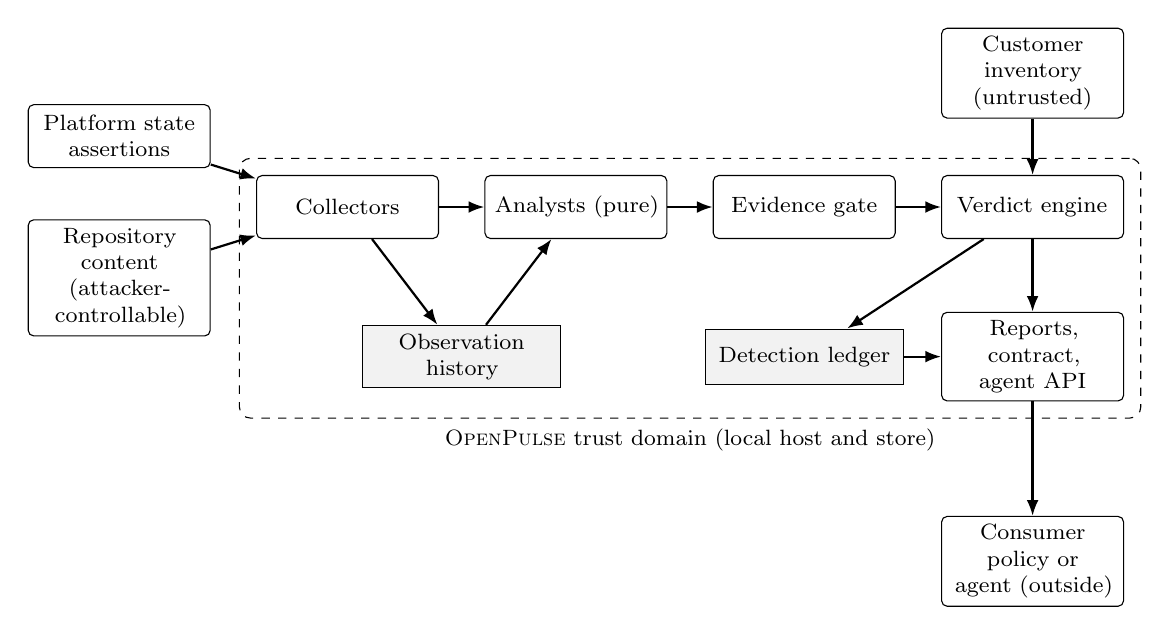
\begin{tikzpicture}[
  box/.style={draw, rounded corners=2pt, align=center, font=\footnotesize,
              minimum height=8mm, inner sep=3pt, text width=2.1cm},
  store/.style={draw, align=center, font=\footnotesize, inner sep=3pt,
                minimum height=7mm, fill=black!5, text width=2.3cm},
  arr/.style={-{Latex[length=2mm]}, thick},
  bound/.style={draw, dashed, rounded corners=4pt, inner sep=6pt}
]
\node[box] (src) at (0,0.9) {Platform state assertions};
\node[box] (content) at (0,-0.9) {Repository content (attacker-controllable)};
\node[box] (col) at (2.9,0) {Collectors};
\node[box] (ana) at (5.8,0) {Analysts (pure)};
\node[box] (gate) at (8.7,0) {Evidence gate};
\node[box] (ver) at (11.6,0) {Verdict engine};
\node[box] (inv) at (11.6,1.7) {Customer inventory (untrusted)};
\node[store] (hist) at (4.35,-1.9) {Observation history};
\node[store] (led) at (8.7,-1.9) {Detection ledger};
\node[box] (out) at (11.6,-1.9) {Reports, contract, agent API};
\node[box] (cons) at (11.6,-4.5) {Consumer policy or agent (outside)};
\draw[arr] (src) -- (col);
\draw[arr] (content) -- (col);
\draw[arr] (col) -- (ana);
\draw[arr] (ana) -- (gate);
\draw[arr] (gate) -- (ver);
\draw[arr] (inv) -- (ver);
\draw[arr] (ver) -- (out);
\draw[arr] (out) -- (cons);
\draw[arr] (col) -- (hist);
\draw[arr] (hist) -- (ana);
\draw[arr] (ver) -- (led);
\draw[arr] (led) -- (out);
\node[bound, fit=(col)(ana)(gate)(ver)(hist)(led)(out),
  label={[font=\footnotesize]below:{\op{} trust domain (local host and store)}}] {};
\end{tikzpicture}
\caption{Pipeline and trust boundaries. Platforms are trusted to
report their own \emph{state} truthfully at query time: canonical
path, archived flag, tag list. They are not trusted to be complete or
current. Repository and advisory \emph{content}, such as descriptions,
release notes and names, is attacker-controllable and is treated as
data, never as instructions. The stores protect only against accidental
corruption. Policy is outside \op{}.}
\label{fig:pipeline}
\end{figure}

\subsection{Observation, claim, event}
An \emph{observation} records what a source exposed at time $t$. A
\emph{claim} is an assertion that names its supporting evidence. An
\emph{event} is a gated, scoped and dated unit of intelligence. A diff
between observations is only a candidate change, with an explicit
evidence strength, until it is gated.

\subsection{Authority, independence and confidence}
Sources are tiered as official, primary, secondary or tertiary.
Authority is claim-specific in principle: GitHub is authoritative for a
repository's canonical path, not for why it moved. Corroboration counts
independent source families, folding derivation chains, and NVD and OSV
count as one family. Where no family is declared, the implementation
falls back to the source name, so undeclared copies of one origin can
count as independent. Confidence (\textsc{Unverified} $<$
\textsc{Emerging} $<$ \textsc{Corroborated} $<$ \textsc{Confirmed}) and
impact (\textsc{Informational} $<$ \textsc{Watch} $<$ \textsc{Review}
$<$ \textsc{Action} $<$ \textsc{Critical}) are \emph{policy categories},
not calibrated probabilities. Table~\ref{tab:caps} collects every rule.
A verdict's confidence is
\begin{equation}
\label{eq:conf}
\mathrm{conf}(d,e) = \min\bigl(\mathrm{ceil}(\mathrm{level}(d,e)),\;
  \mathrm{conf}(e),\; \mathrm{cap}_{\mathrm{id}}(d,e)\bigr).
\end{equation}
Here $L = (\textsc{Unverified} < \textsc{Emerging} <
\textsc{Corroborated} < \textsc{Confirmed})$ is a total order, and
$\min$ is its meet. $\mathrm{conf}(e) \in L$ is the gated event
confidence. $\mathrm{ceil}$ maps the verdict's match level to $L$ by
the ``match ceiling'' row of Table~\ref{tab:caps}.
$\mathrm{cap}_{\mathrm{id}}(d,e)$ is \textsc{Emerging} when the verdict
is affected through a \textsc{Review-Required} or \textsc{Unverified}
identity mapping, other than by exact artefact equality, and
\textsc{Confirmed} (no effect) otherwise. The equation is normative,
and it is also what the implementation computes
(\code{core/risk/check.py}). Impact is copied from the gated event and
never raised by the verdict engine. Equation~\eqref{eq:conf} involves
no numerical thresholds. It takes the minimum over an ordinal scale,
so each cap can only lower a verdict's confidence. Neither confidence
nor impact has a numerical interpretation, in outputs or in
evaluation tables. The ceilings and caps are design choices, not
calibrated values. Whether they separate reliable verdicts from
uncertain ones is measured by the stratified error rates in
Appendix~\ref{app:protocol}.

\begin{table}[t]
\centering
\small
\begin{tabularx}{\linewidth}{@{}l X@{}}
\toprule
Stage & Rule \\
\midrule
Event confidence & \textsc{Confirmed}: official evidence (official or primary
  for lifecycle classes). \textsc{Corroborated}: $\ge$2 independent families.
  \textsc{Emerging}: one credible source. \textsc{Unverified}: otherwise. \\
Gate & \textsc{Unverified} $\Rightarrow$ impact $\le$ \textsc{Watch};
  \textsc{Emerging} $\Rightarrow$ $\le$ \textsc{Review};
  \textsc{Action}/\textsc{Critical} need $\ge$ \textsc{Corroborated};
  artefact classes must name artefacts; dated classes need dates;
  unresolved contradiction blocks \textsc{Action}/\textsc{Critical}. \\
Vulnerabilities & Keyword-only match $\le$ \textsc{Review}; KEV with
  undetermined applicability $\Rightarrow$ \textsc{Review}. \\
Match ceiling & object, repository, exact namespace or tag
  $\to$ \textsc{Confirmed}; version, not-affected $\to$
  \textsc{Corroborated}; package, project $\to$
  \textsc{Emerging}; related, unknown, and any envelope membership
  $\to$ \textsc{Unverified}. \\
Identity cap & Affected through a \textsc{Review-Required} or
  \textsc{Unverified} mapping $\Rightarrow$ $\le$ \textsc{Emerging}. \\
\bottomrule
\end{tabularx}
\caption{All confidence and impact rules.}
\label{tab:caps}
\end{table}

\subsection{Temporal roles and lead time}
\label{sec:temporal}
Five roles are kept apart: \emph{announced} (from sources with a
trustworthy publication date, otherwise unknown), \emph{effective},
\emph{first detected}, \emph{last verified} and \emph{reported}.
Conflicting effective dates are preserved as separate evidence.
Detection lead is
$\mathrm{lead}(c) = \mathrm{effective}(c) - \mathrm{firstDetected}(c)$
in days. Positive means advance warning, negative means a measured late
detection, and the lead is undefined only when a term is unknown. A lead
depends on when monitoring started and how often it polls, so it is an
\emph{instrument capability and evaluation metric}, not an established
benefit.

\paragraph{Freshness and supersession.} A historical observation
presented as current can mislead, for instance about where a
repository now lives or whether a tag still resolves. We specify
freshness per event class $c$ and dependency role $r$ with a policy
bound $\tau_{c,r}$ (below). An observation is \emph{fresh} while its
last successful acquisition is within that bound of the evaluation
time, and not later than it. A failed acquisition records a
gap and never refreshes it. An event is \emph{current} if its
\emph{last verified} date is fresh and no later event from the same
source corrects, withdraws or supersedes it. A negative verdict is
admissible only from a current event. From a stale event the verdict
is \textsc{Related}, with the reason \emph{stale} kept distinct from
\emph{undetermined}, so that a consumer can tell old evidence from
unresolved evidence. A withdrawn advisory asserts nothing.

In the implementation, verdicts are recomputed from the loaded events
on every run, and nothing stores a negative for reuse, so a corrected
event changes the next run's verdict. The contract exports
\code{last\_verified}. Withdrawn OSV entries are skipped, and withdrawn
or superseded events are not evaluated. The bound is one maximum
evidence age, not one per class. Given an evaluation time, a negative
from an event whose \emph{newest} evidence is older becomes
\textsc{Related}, with the reason \emph{stale}. This is weaker than the
specification. One recently acquired item makes the whole event fresh,
however old the others are, and the completeness declaration and the
identity mapping carry no date that the check reads; two of the
retrospective study's events (DIS-1, DIS-4) were fresh only through
their newest item. The check applies to event-scope negatives only. Advisory-path
negatives bypass it; this gap is open.

The command line's verdict commands (\code{check}, \code{attest},
\code{digest}, \code{warnings}) and the agent tools apply a 90-day
bound by default, as of the start of the current day. \code{--replay},
or replay mode in the agent's Python API, drops the bound and says so,
because replaying recorded evidence offline would otherwise make every
negative stale. Contracts record the frame in
\code{evaluation\_context}. The library call (\code{check\_dependency})
applies a bound only when the caller passes one. The 90-day value is a
placeholder: in the retrospective study it changed no decision, and it
is not calibrated to any event class. An evaluation time in the past
(\code{--as-of}) is a reference point for the bound, not a knowledge
cut. Evidence acquired after it is still used, so a past date can give
a negative that nothing known at that date supported. This gap is open;
the evaluation harness avoids it by cutting knowledge first. The
report-placement
freshness classes in \code{core/freshness.py} decide whether a change
is \emph{news}. They are not evidence currency and do not gate
verdicts.

Three levels of currency are kept apart: (i)~\emph{evidence recently
fetched}; (ii)~\emph{claims recently revalidated}, that is, re-derived
from a re-acquired response whose upstream state is itself current;
and (iii)~\emph{a verdict still valid when consumed}. By default the
implementation establishes part of~(i): the newest item of an event is
no more than 90 days old. It establishes~(ii) only for lifecycle
events the agent derives live from a freshly fetched response, and
even then not the upstream's own currency. Curated events,
completeness declarations and identity mappings are never revalidated.
It does not establish~(iii): an exported contract has no expiry or
supersession. Recomputation is not freshness either. A verdict
recomputed today from an observation acquired weeks ago is as old as
that observation, and the agent interface reuses each fetched
response, successful or failed, for up to an hour
(Section~\ref{sec:consumers}). If a source is unavailable, its
acquisitions are recorded as gaps and the events already loaded stay
in force; nothing withdraws their negatives
(Section~\ref{sec:limits}).

Event classes need different currency rules. A relocation is a
historical fact. Its observation stays true of the time it was made,
and what can go stale is whether the redirect still holds. Availability
of a tag or image is a current state, and needs a short bound. A
scheduled lifecycle statement is valid until its source revises it, and
needs re-verification of the schedule, not of the date. Currency is
also a property of what a negative \emph{depends on}, not of the event
as a whole: the evidence that defines the event's scope, the
completeness declaration and the item supporting its basis, and, for
an exclusion on identity grounds, the dependency's curated mapping
(Section~\ref{sec:identity}). Each must be fresh under
$\tau_{c,r}$; a role may need only non-supersession, as for a
historical relocation's announcement. The implementation does not
record which item plays which role. Taking the oldest item instead is
no substitute: in the retrospective study it would have withheld six
correct negatives of the relocation events DIS-1 and DIS-4. There is also
a time-of-check to time-of-use gap across the decision points of
Section~\ref{sec:problem}. A fresh answer before adoption says nothing
about the state at installation. A bounded implementation therefore
binds each assessment to the exact reference, ideally a digest, and to
its evaluation context and acquisition time. Stage~2 must re-evaluate
it rather than reuse a stage-1 answer. After a failed acquisition, no
cached negative is reused silently: the result is \emph{stale} or
\emph{unavailable}, and both are distinct from undetermined.

\subsection{Evidence integrity}
\label{sec:integrity}
Registry observations are hash-chained,
$H_n = \mathrm{SHA256}(\mathrm{canon}(o_n) \| H_{n-1})$, and broken
chains are never diffed against. A change to acquisition semantics
bumps a parser version and forces a re-baseline. First detections are
earliest-witness ledger entries whose content hash is verified on
read. The hashes are unkeyed. They detect accidental and partial
corruption, not a writer who rewrites the suffix, rolls back, or
backdates a fact. Rollback and backdating resistance need witnesses
outside the operator's control, such as a monotonic counter or the
chain tip anchored in an external log~\cite{rfc9162}. A keyed MAC
alone would not prevent replay of an older store. The guarantee is
therefore \emph{integrity against accidental and partial corruption
only}. It establishes neither authenticity (who wrote the evidence),
nor freshness, nor rollback resistance, and a privileged local
operator, or a compromised host, is outside the adversary it resists.
We call the stores hash-chained rather than tamper-evident for this
reason.

\section{Q2b: Applying Evidence --- Applicability Specification}
\label{sec:applicability}

\subsection{What a verdict means}
\label{sec:meaning}
Four predicates are kept apart: (a)~\emph{object equality};
(b)~\emph{scope membership}; (c)~\emph{availability}, meaning that a
reference resolves under stated conditions; and (d)~\emph{consequence}
for the dependent system. \emph{Affected}$(d,e)$ means (b).
\textsc{NotAffected}$(d,e)$ means only that $d$ is outside $e$'s
\emph{directly named} scope. It says nothing about availability,
maintenance or vulnerability, and nothing about other events.
Table~\ref{tab:verdicts} states what each verdict asserts and what is
required before it may be issued. Every condition in its last column
is checked in code and exercised by the build gate
(Section~\ref{sec:audit}).

\begin{table}[t]
\centering
\footnotesize
\begin{tabularx}{\linewidth}{@{}>{\raggedright\arraybackslash}p{2.5cm} >{\raggedright\arraybackslash}X >{\raggedright\arraybackslash}X@{}}
\toprule
Verdict & Asserts & Required before it may be issued \\
\midrule
\textsc{Affects*} & $d$ is in the event's scope & Membership in an
  \emph{exact} element, after canonicalisation; for versions, a
  comparison under the range's own scheme \\
\textsc{Affects\-Project} & $d$ belongs to the event's project; scope
  membership not established & Identity resolved to the project; no
  exact member, nothing undetermined \\
\textsc{Related} & An association exists but is not established &
  Any element undetermined: envelope membership, unresolved identity,
  incomparable version, mixed pinning, unknown tag, or a negative
  withheld (partial scope, missing basis, stale or contested event) \\
\textsc{Not\-Affected} & $d$ is outside the directly named scope &
  N1--N5: every element excludes; identity exclusion only through a
  curated mapping; complete scope with recorded basis; fresh and
  uncontested event \\
\textsc{Unknown} & No association & $d$ is curated as another project
  against identity-defined elements, or no element relates to it;
  never because identity is unresolved or untrusted (D16 open) \\
\bottomrule
\end{tabularx}
\caption{Verdict semantics. Across events, a dependency is affected if
any event affects it, cleared only if every associated event gives
\textsc{NotAffected}, and unresolved otherwise (Table~\ref{tab:xevent}).}
\label{tab:verdicts}
\end{table}

Whether an event reaches a downstream distribution or an embedded
component must come from the event's definition, not from identity
modelling alone. An upstream end-of-life statement may concern the
upstream's maintenance obligations, not a vendor's support of a
repackaged image. A ``contains'' relation would let \op{} ask the
question, but containment should not propagate every event
automatically. Each relation needs event-specific rules. A negative
verdict should therefore carry three distinct statements: outside the
directly named scope; embedded-component relation not evaluated; and
operational or security consequence not evaluated. Agents in
particular may read a bare \textsc{NotAffected} label as permission to
proceed. Contract 1.2.0 carries the three statements as
\code{verdict\_meaning}.

The same boundary applies to positives. \textsc{AffectsArtifact} means
scope membership, not that a reference is broken, unsafe, vulnerable or
unmaintained. Case~10 (Table~\ref{tab:spark}) shows that a tag listing
can establish a distribution change without establishing whether a
particular reference still resolves. The contract should therefore
carry four separate fields, each with its own evidence or an explicit
\emph{not evaluated}: direct scope membership; observed availability or
resolution; maintenance or support implication; and security
consequence, only where it is independently established. That would
stop a downstream policy from turning a correct membership result into
an unsupported security conclusion. Contract 1.2.0 carries them as
\code{verdict\_meaning}: direct scope, with embedded
components, availability, maintenance and security consequence marked
\emph{not evaluated}. Evidence-bearing values for the last four are not
yet produced.

\subsection{Typed scope}
\label{sec:scope}
An event $e$ has a scope $S(e) = (E, \chi, \beta)$: a finite set $E$
of typed elements, a completeness state $\chi$, and the basis $\beta$
of that state (Section~\ref{sec:scope}, \emph{Completeness}). Each
element has one kind,
and the denotation $\llbracket x\rrbracket$ of an element is the set of
dependency references it covers:
\begin{description}[leftmargin=*,font=\normalfont\itshape,nosep]
  \item[project $p$:] every reference that resolves to project $p$.
    It is always an envelope (below): it gives a contextual tie, never
    a positive, and is never used for exclusion.
  \item[repository $r$:] every reference to repository $r$, whatever
    its tag or digest. Repository-wide changes such as relocation and
    withdrawal use this kind.
  \item[namespace $g/n/{*}$:] every repository under namespace $n$ of
    registry $g$. Catalogue-wide changes use this kind, for example
    \code{docker.io/bitnami/*}, instead of listing example images that
    would wrongly be read as the complete scope.
  \item[tag $r{:}t$:] references to $r$ that carry exactly tag $t$. In
    place of a literal tag, an element may carry a tag predicate:
    \code{<version>} denotes every version-like tag (\code{1.25},
    \code{7.2.4-debian-12-r3}, not \code{latest}), and \code{*} every
    tag. A predicate applies to a repository or a namespace, so
    \code{docker.io/bitnami/*:<version>} is every versioned image
    under the namespace. A reference with no tag is read as
    \code{latest}.
  \item[release line $(p, \ell)$:] versions of project $p$ inside line
    $\ell$ (\code{4.2} covers \code{4.2.11}, not \code{4.20.1}).
  \item[object $r@h$:] the content object with digest $h$, together
    with its OCI level (index, manifest or layer).
  \item[package $(\mathit{eco}, n)$:] every reference to package $n$ in
    ecosystem $\mathit{eco}$.
  \item[registry $g$:] every reference served by registry $g$, for a
    registry-wide change such as a service withdrawal or an
    authentication change.
\end{description}
Each element also has a \emph{role}. An \emph{exact} element claims
$\llbracket x\rrbracket \subseteq A_e$: everything it denotes is in
scope. An \emph{envelope} element claims only that it helps cover
$A_e$. It may include unaffected references, so it can justify an
exclusion but not a positive. Coverage and exactness are different
premises (Section~\ref{sec:soundness}). One completeness declaration
justifies negatives and says nothing about positives. The Bitnami
withdrawal shows why. The versioned images moved, but \code{latest}
stayed in the mainline. The namespace \code{docker.io/bitnami/*} is
therefore a correct envelope, and an inexact one, since it contains
\code{bitnami/redis:latest}. An exact representation pairs that
envelope with an exact element for the versioned tags under the
namespace, \code{docker.io/bitnami/*:<version>}. A tag element alone
would not remove \code{latest} from the namespace union. Roles follow
from an element's form. Three forms are envelopes: a project, a
namespace without a tag predicate, and a registry (the representation
has no exact registry form). Every other form is exact, including a
namespace with a predicate.

Each element also has a \emph{purpose} $\pi(x) \in \{\text{bound},
\text{example}\}$, so $E = E_B \uplus E_X$. A \emph{bounding} element
takes part in the coverage claim: $\chi$ is a statement about $E_B$
alone. An \emph{example} is one of \op{}'s named
\code{affected\_artifacts} (a repository, tag, object or source
repository). Membership in it is a positive, but it bounds nothing, so
where a bounding element of its form gives \Non{}, an example gives
\Ind{} for the same repository and \NoA{} otherwise
(Table~\ref{tab:membership}). Project-wide scope is an explicit
project element, so $E = \emptyset$ means an event that names nothing,
not ``the whole project''.

\paragraph{Completeness.} $\chi \in \{\text{verified}, \text{declared},
\text{partial}\}$. \emph{Verified}: the acquisition and
scope-construction procedure shows that $E$ covers the affected set,
under stated assumptions traceable to the exact responses and
pagination state. \emph{Declared}: a producer asserts it.
\emph{Partial}: not established. A deployment policy chooses the
admissible states $\mathcal{A}$ for negatives: $\{\text{verified}\}$
for high assurance, or $\{\text{verified}, \text{declared}\}$ under a
labelled weaker policy. In \op{} completeness is opt-in. An unspecified
scope is partial. Analysts declare completeness only where the scope
is the event itself, such as one release line reaching end of life or
one repository's distribution change. Curated events declare it
explicitly. No verifier exists yet, so the implemented policy is
$\mathcal{A} = \{\text{declared}\}$.

A well-formed declaration is not an independently justified one. A
declaration is an assertion. Its only support is the evidence behind
the event, and a wrong curated event, a misread announcement or a
compromised producer can declare an incomplete scope complete. Then
(P1) fails and a negative can be a false clear (Section~\ref{sec:soundness}).
\op{} cannot distinguish a declaration from evidence for it, but it
records what the declaration rests on. The specification therefore treats the basis as a
first-class security input. Declared completeness splits into two
bases that carry different evidence. A \emph{definitional} scope is
complete because it is the event itself: one release line reaching end
of life, or one repository's distribution change. An \emph{announced}
scope is complete because a named source says so. A declaration
records its source, the scope definition, an evidence reference, the
observation time and the validation method, if any. The specification
requires the contract to carry $\chi$ and that record next to every
negative. Each scope records its basis (\code{definitional},
\code{announced}, \code{corroborated} or \code{verified}), and a
declaration without one never clears. Contract 1.2.0 carries the
completeness state, its basis and whether it admits a negative; the
source, evidence reference and validation method are not carried
(Section~\ref{sec:consumers}).

The admissibility condition is then machine-checkable. A negative is
admissible iff every scope element is decisively excluded and the pair
$(\chi, \beta)$ is in the consumer's admissible set $\mathcal{A}$, a
set of (state, basis) pairs.
Table~\ref{tab:policies} gives each state's evidence requirement, and
what a consumer who admits it is trusting. Policies are combinations
of rows. \emph{High assurance} admits only verified scopes, so it
issues no negatives today. \emph{Definitional} admits verified and
definitional scopes. \emph{Implemented} also admits announced scopes,
which is the implemented behaviour. The bases are recorded and told
apart there, but the implementation admits every recorded basis, so a
consumer cannot yet select a stricter set. The evaluation reports error rates separately per
basis rather than pooling them (Appendix~\ref{app:protocol}).

\begin{table}[t]
\centering
\footnotesize
\begin{tabularx}{\linewidth}{@{}>{\raggedright\arraybackslash}p{2.3cm} >{\raggedright\arraybackslash}X >{\raggedright\arraybackslash}X >{\raggedright\arraybackslash}p{2.1cm}@{}}
\toprule
State (basis) & Evidence required & Consumer who admits it trusts & Supports a negative \\
\midrule
Verified & A procedure binding $E$ to the exact responses and
  pagination state & The procedure and the platform's state assertions
  & Yes if labelled, but no verifier checks the label \\
Declared (definitional) & The event's own definition; one release
  line or one repository & That the event is correctly typed & Yes \\
Declared (announced, corroborated) & The announcement, plus an
  independent source family stating the same extent & Two independent
  sources, and our reading of them & Yes \\
Declared (announced) & A named source's announcement, with an
  evidence reference & That source, and our reading of it & Yes \\
Partial & None & -- & Never: exclusion from known members is not a
  clearance (D4) \\
\bottomrule
\end{tabularx}
\caption{Completeness states, the evidence each requires, and what a
consumer admitting it trusts. Corroboration counts source families,
not names (Section~\ref{sec:model}). If two sources disagree on the
extent of a scope, the scope is partial until the conflict is resolved.
\op{} detects a conflict within one event's evidence (a
\emph{contradicts} relation), not between separate events.}
\label{tab:policies}
\end{table}

\paragraph{Completeness is never derived from a listing.} Could a
compromised or misbehaving registry serve a partial tag listing, or a
truncated pagination state, so that \op{} declares a scope complete
that is not, and thereby manufacture a false clear? The claim we can
support is narrower than ``it cannot''. It is a dataflow invariant we
checked in the code. Completeness is declared at seven
analyst sites in \code{analyzers/change\_analyst.py} and in curated
fixtures. Every analyst site builds $E$ from the analysed subject
itself: the release line, version or repository that was probed. None
builds it from the members of an enumeration. So the \emph{size} of a
listing never enters $E$ or $\chi$. A manipulated listing can still
change \emph{whether} an event exists. That can cause a missed
detection, or a false impact (a phantom removal, if the partiality goes
undetected). And because a missing event drops out of the cross-event
summary, it can change which events a summary is taken over. What we
have not shown is an end-to-end argument that listing manipulation
cannot alter event identity, scope construction, declaration choice or
the loaded event set by some other route. The invariant is not yet a
regression test. Same-host pagination, the page cap, the v2 fallback
and the \code{truncated} flag reduce particular acquisition failures.
They do not prove that a listing is complete, or that its sources are
independent. A listing that is incomplete in a way the walk cannot
detect remains a threat to discovery (Table~\ref{tab:threats}). A
future \emph{verified} state would have to bind completeness to the
exact responses and pagination state, and would inherit exactly this
threat.

\subsection{Membership tests}
\label{sec:tests}
A test $t(d,x)$ returns \Mem{} (member, with a match level), \Non{}
(decisively excluded), \Ind{} (undetermined), \Proj{} (project tie)
or \NoA{} (no association):
\begin{description}[leftmargin=*,font=\normalfont\itshape,nosep]
  \item[Project.] \Proj{} if $d$ resolves to $p$. \NoA{} if $d$
    resolves through a curated \textsc{Verified} mapping to another
    project; \Ind{} for a heuristic or unreviewed mapping (D16 is the
    open exception, Table~\ref{tab:defects}). \Ind{} if $d$'s identity is unresolved, including a reference that
    resolves only to itself, whatever its name: a mirror, fork or
    rename can be called anything. \code{github.com/etcd-io/etcd}
    against etcd is one such case.
  \item[Repository.] \Mem{} if $d$ names $r$, whatever its tag or
    digest. Otherwise \Non{}.
  \item[Namespace.] \Mem{} if $d$'s registry and namespace are $g$ and
    $n$. Otherwise \Non{}.
  \item[Tag.] \Mem{} if $d$ is $r{:}t$. \Non{} if $d$ is $r{:}t'$ with
    $t' \ne t$, or another repository. \Ind{} if $d$ pins a digest of
    $r$, because a tag can move.
  \item[Release line.] \NoA{} if $d$ resolves through a curated
    mapping to a project other than $p$, and \Ind{} if its identity is
    unresolved or the resolution is untrusted. Otherwise compare versions: inside gives
    \Mem{}, outside gives \Non{}, not comparable gives \Ind{}.
  \item[Object.] Equal digests give \Mem{}. For unequal digests the
    answer depends on the levels. If $x$ is an index and $d$ pins one
    of its children, then \Mem{} if the event covers \emph{all}
    children (or the deployment-selected platform's child), otherwise
    \Ind{}. If $x$ is a manifest and $d$ pins the parent index, the
    result is \Ind{}: the deployment's platform selection decides
    whether the event's platform is used. \Non{} only if both levels
    are known and neither contains the other. If either level is
    unknown, \Ind{}.
  \item[Package, registry.] Names are compared in canonical form:
    lowercase, with PEP~503 folding for PyPI and Maven
    \code{groupId:artifactId} read as \code{groupId/artifactId}. Equal
    names give \Mem{}. Unequal names give \Ind{}, because other
    spellings (npm scopes, Go module paths) are not canonicalised, or
    \NoA{} if $d$ is curated as another project. A value written as a
    purl decides by ecosystem and name: the same package gives \Mem{},
    a package of another ecosystem gives \Non{}, and another name in
    the same ecosystem gives \Ind{} (F1--F3,
    Appendix~\ref{app:repro}). A registry element is an envelope: the
    same registry gives \Ind{}, a different registry gives \Non{}.
  \item[Envelopes and examples.] Membership in an envelope gives \Ind{}
    (\Proj{} for a project element) instead of \Mem{}; non-membership
    is still \Non{}. A tag-restricted element gives \Ind{} for a
    reference that pins only a digest, since its tag is unknown. An
    example never gives \Non{} (Section~\ref{sec:scope}). Named and
    bounding elements are evaluated together, and the strongest result
    wins.
  \item[Identity versus location.] Identity decides only elements
    whose denotation is defined \emph{through} a project: project,
    release line, and a bare package value (F3). For these, a curated
    \textsc{Verified} mapping of $d$ to another project gives \NoA{},
    which needs no complete scope. Location elements (repository, tag,
    namespace, object, registry, source repository) are decided by
    location, never by $d$'s project: a reference of another project
    that resides in an affected repository, namespace or registry is a
    member.
  \item[Across reference kinds.] A package reference gives \NoA{}
    against container-image, object and registry elements unless it
    resolves to the event's project (then \Ind{}, or \Proj{} against a
    registry), since a package is never one of those. A Go module gives \Ind{} against a
    source-repository element, whatever its identity, because it may
    live in the repository under any path; another package gives \NoA{}.
    A Go module at or below a named repository path, directly or by the
    \code{gopkg.in} and \code{golang.org/x} conventions, gives \Mem{};
    positive only, since a vanity path may name the same repository
    (D-R1 in Table~\ref{tab:since}; Section~\ref{sec:retro}). Any other comparison across kinds
    gives \Ind{}. The element-specific rules above apply only when the
    kinds agree. Appendix~\ref{app:membership} gives the normative
    table of forms, roles, purposes and results, and two places where
    the release departs from it.
\end{description}

\begin{algorithm}[t]
\caption{Applicability of event $e$ to dependency $d$}
\label{alg:agg}
\begin{algorithmic}[1]
\Function{Applicability}{$d, e$}
  \If{$e$ is withdrawn or superseded}
    \State \Return \textsc{Unknown} \Comment{layer 1: not evaluated (N4)}
  \EndIf
  \State $(E, \chi, \beta) \gets S(e)$; \quad $T \gets \{\, t(d,x) : x \in E \,\}$
  \Comment{every element, no early return}
  \If{$\Mem \in T$} \State \Return \textsc{Affects}(strongest member level) \EndIf
  \If{$\Ind \in T$} \State \Return \textsc{Related} \EndIf
  \If{$\Non \in T$}
    \If{$T \subseteq \{\Non, \NoA\} \wedge (\chi, \beta) \in \mathcal{A} \wedge e$ is fresh and uncontested}
      \State \Return \textsc{NotAffected} \Comment{layer 1 for negatives (N4, N5)}
    \EndIf
    \State \Return \textsc{Related} \Comment{exclusion from a scope not known to be complete}
  \EndIf
  \If{$\Proj \in T$} \State \Return \textsc{AffectsProject} \EndIf
  \State \Return \textsc{Unknown} \Comment{$T \subseteq \{\NoA\}$, including $E = \emptyset$}
\EndFunction
\end{algorithmic}
\end{algorithm}

Algorithm~\ref{alg:agg} has three layers, and the executable oracle
must implement all of them. Conformance of the second and third layers
alone would validate a weaker kernel than the policy this report
states. Layer~1 decides event admissibility. A withdrawn or
superseded event is not evaluated. A stale or contested event may
still associate a dependency, but it may never clear one. Layer~1
never changes a positive. Layer~2 is the per-element tests,
on canonical references. Layer~3 is per-event aggregation, followed by
the cross-event summary below. Layer~1 drops withdrawn and superseded
events, withholds negatives from events contested by their own
evidence, and applies the freshness bound (Section~\ref{sec:temporal}).

\paragraph{Across events.} $d$ is \emph{affected} if any event affects
it, \emph{cleared} only if every event with an association returns
\textsc{NotAffected}, and \emph{unresolved} otherwise. Events returning
\textsc{Unknown} carry no association and are left out. In the
specification that is safe, because \NoA{} requires a \textsc{Verified}
resolution to another project, and an unresolved identity yields \Ind{}
and therefore \textsc{Related}. The implementation used to detect
unresolved identity only by name, and that was defect D10
(Table~\ref{tab:defects}). With the etcd relocation and Bitnami events
loaded, an unmapped \code{docker.io/zzz/kvstore} was summarised as
\textsc{NotAffected}, while \code{docker.io/zzz/etcd} was
\textsc{Related}. In that reproduction no pair verdict was
\textsc{NotAffected}, but the user-facing consequence was the same as
a false clear. A second reproduction of D10 was a pair-level false
clear: under a version-scoped event, the unmapped reference was
excluded on identity grounds (Appendix~\ref{app:defects}). Since
\dninecommit{}, every unmapped reference yields \Ind{}; a heuristic
mapping to another project still drops out (D16, open).

\paragraph{Cross-event aggregation as a separate property.} Per-event
soundness does not imply a sound summary: D3 was a summary that
displayed a clearance while another event was unresolved. The summary
must keep three outcomes apart. \emph{No association exists}
(\textsc{Unknown}, from \NoA{}). \emph{An association was not
established} (\textsc{Related} or \textsc{AffectsProject}, from
\Ind{} or \Proj{}). \emph{Decisively excluded} (\textsc{NotAffected}).
Table~\ref{tab:xevent} is the truth table over the set $R$ of
per-event results. The property is that the summary is \emph{cleared}
only if $R \subseteq \{\textsc{NotAffected}, \textsc{Unknown}\}$ and
$\textsc{NotAffected} \in R$. The implementation's summary function
takes a maximum over seven distinct ranks and then filters a set.
Its result is therefore order-independent and idempotent: it depends
only on which relationships occur, not on their order or multiplicity.
There are 127 non-empty such sets. We checked every ordering of each
of them (13{,}699 sequences), and every sequence of one to five results
with repetition (19{,}607), against Table~\ref{tab:xevent}, with no
mismatch (\code{papers/tr-2026-01/check\_aggregation.py}). With the
order-independence argument, this covers inputs of any length. It
covers the summary step only. That an unresolved association reaches
the summary as \textsc{Related} rather than \textsc{Unknown} is a
separate property, which the D10 regression tests pin.

The table needs no further rows for the harder cases, because each of
them is decided per event before aggregation. An event with a partial
scope, unresolved identity, a contradiction about its extent, or
stale evidence gives \textsc{Related} for $d$. A withdrawn or
superseded event is not loaded, and contributes nothing. Two events
with conflicting scopes are two per-event results, and the table
combines them. The specification therefore guarantees that a negative
from one event never erases uncertainty from another. A conflict
between separate events is not detected (Section~\ref{sec:limits}).

The summary is taken over the \emph{loaded} event set, and that limits
what ``cleared'' can mean. It states that every loaded event that
associates with $d$ excludes it. It does not state that no relevant
change exists under adequate monitoring coverage: an event that
discovery missed, that a manipulated listing suppressed, or whose
acquisition failed is simply absent, and the table cannot see an
absence (Table~\ref{tab:adversary}, row 7). Neither the summary label
nor contract 1.2.0 records the loaded set's coverage. A consumer must read a
clearance as ``excluded by the events we have'', and a coverage field
that says which sources and event classes were current at evaluation
time is needed before a summary can support more.

\begin{table}[t]
\centering
\footnotesize
\begin{tabularx}{\linewidth}{@{}>{\raggedright\arraybackslash}X l@{}}
\toprule
Per-event results $R$ (any number of events) & Summary \\
\midrule
Some \textsc{Affects*} (artifact, version or package) & affected \\
No \textsc{Affects*}; some \textsc{Related} or \textsc{AffectsProject} & unresolved \\
Only \textsc{NotAffected} and \textsc{Unknown}, at least one \textsc{NotAffected} & cleared \\
Only \textsc{Unknown} (including no events) & no association \\
\bottomrule
\end{tabularx}
\caption{Cross-event aggregation. A clearance never headlines over an
unresolved association, whatever the order or number of events.}
\label{tab:xevent}
\end{table}

\subsection{Soundness of negative verdicts}
\label{sec:soundness}
Let $A_e$ be the set of dependency references that are truly in scope
of the upstream change described by $e$, at the time of evaluation.

\begin{lemma}[Aggregation]
\label{lem:agg}
Assume (P1)~\emph{coverage}: if $(\chi, \beta) \in \mathcal{A}$ then
$A_e \subseteq \bigcup_{x \in E_B} \llbracket x \rrbracket$; and
(P2)~\emph{test soundness}: $t(d,x) \in \{\Non, \NoA\} \Rightarrow
d \notin \llbracket x \rrbracket$. If Algorithm~\ref{alg:agg} returns
\textsc{NotAffected} for $d$, then $d \notin A_e$.
\end{lemma}
\begin{proof}
\textsc{NotAffected} is returned only when $(\chi, \beta) \in
\mathcal{A}$ and $t(d,x) \in \{\Non, \NoA\}$ for every $x \in E$. By
(P2), $d \notin \llbracket x\rrbracket$ for every $x$. Hence
$d \notin \bigcup_{x \in E_B} \llbracket x \rrbracket \supseteq A_e$
by (P1), since $E_B \subseteq E$.
\end{proof}
P2 for an identity-based \NoA{} needs a correct curated mapping, and
holds only because identity decides identity-defined elements alone
(Section~\ref{sec:tests}). For a location element, a correct mapping
to another project does not imply $d \notin \llbracket x\rrbracket$.

Coverage makes $\bigcup_x \llbracket x\rrbracket$ an over-approximation
of $A_e$, so it justifies negatives only. Positives need a separate
premise.

\begin{lemma}[Positives]
\label{lem:pos}
Assume (P3)~\emph{exactness}: $\llbracket x\rrbracket \subseteq A_e$
for every exact element $x$; and (P4)~\emph{membership soundness}:
$t(d,x) = \Mem \Rightarrow d \in \llbracket x\rrbracket$, where
$t(d,x) = \Mem$ only for exact $x$. If Algorithm~\ref{alg:agg} returns
\textsc{Affects} for $d$, then $d \in A_e$.
\end{lemma}
\begin{proof}
\textsc{Affects} is returned only when $t(d,x) = \Mem$ for some
element $x$, which is exact. Then $d \in \llbracket x\rrbracket
\subseteq A_e$ by (P4) and (P3).
\end{proof}

Neither lemma needs the other's premises. A system can satisfy the
negative premises and violate the positive ones. Before roles were
implemented, \op{} violated (P3): D7 and the Bitnami \code{latest} case
were false impacts. Envelope membership no longer yields a positive, so (P3) rests on the exact elements being exact.
That is a property of the event's curation, which nothing verifies.
Satisfying the positive premises would not make the negatives sound. Its negatives are
sound only where the negative-admission conditions hold, and they are
enforced only with the gaps stated in Section~\ref{sec:soundness}
(\emph{The \textsc{NotAffected} contract}).

The lemma is elementary, and that is intended. It is a compact
correctness argument for the aggregation rule, not the primary
evidence of \op{}'s security, and it implies no more assurance than
its premises carry. The central technical evidence is meant to be
conformance (Section~\ref{sec:audit}), which has been run on a
generated matrix and on random cases.
The research question
is not the implication. It is how an implementation establishes
(P1) and (P2), and Table~\ref{tab:premises} decomposes them. (P1)
requires a faithful event, the right elements, completeness and
currency. (P2) requires correct identity and correct version, tag and
object semantics. Rows marked ``not established'' are the paths by
which a false clear can still occur.

\paragraph{Two counterexamples.} Both premises have failed in
practice, in our own implementation. \emph{(P1) violated:} the Bitnami
event's scope listed five example images, and it was read as complete.
\code{docker.io/bitnami/nginx} is in $A_e$, every element excluded it,
and the verdict was \textsc{NotAffected} (D4). \emph{(P2) violated:} a
Bitnami-packaged \code{postgresql} image was resolved by a namespace
heuristic to a project other than PostgreSQL, so the release-line test
returned \Non{} without an established identity. If the image is a
build of the release line its tag names, it is in the element's
denotation, and the \textsc{NotAffected} verdict was a false clear
(D5). In both cases the aggregation was correct, and the error came
from a premise.

\paragraph{End-to-end statement.} The property the deployed system can
claim is: if \op{} returns \textsc{NotAffected}$(d,e)$ at time $\tau$,
then $d \notin A_e(\tau)$, \emph{provided} that every P1 and P2 row
of Table~\ref{tab:premises} holds for $(d,e)$; P3 and P4 concern
positives only. The inventory premise is outside \op{}, which treats
the inventory as untrusted input. The claim is no stronger than its
weakest row, and the rows marked not established are why this report
makes no unconditional claim about negatives.

\paragraph{The \textsc{NotAffected} contract.} Collected in one place,
a negative verdict for $(d,e)$ is admissible only if all of the
following hold:
(N1)~every element of $E$ gives \Non{} or \NoA{}, after canonicalising
both references; (N2)~any exclusion on identity grounds rests on a
curated mapping of $d$ to a different project, never on a name or a
self-resolution; (N3)~$(\chi, \beta) \in \mathcal{A}$, with the
declaration's basis recorded; (N4)~$e$ is current: every item the
negative depends on (scope-defining evidence, the completeness basis
and any identity mapping used) was acquired no later than the
evaluation time and is fresh under the bound for its class and role
(Section~\ref{sec:temporal}), and $e$ is not corrected, withdrawn or
superseded; and (N5)~no
unresolved contradiction exists about the extent of $E$. Otherwise the
verdict is \textsc{Related} or \textsc{Unknown}, never
\textsc{NotAffected}. Each condition is a check on recorded data, so
the contract is machine-checkable once the data are recorded. (N1)
and (N2) are enforced and regression-tested. (N3) is enforced: a
declaration without a recorded basis never clears. (N4) is enforced
for withdrawn and superseded events, and for freshness under the
90-day default of the command line and agent tools; only the library
call and an explicit replay omit it. The enforced form is weaker than
(N4): one bound for all classes, applied to the event's newest item,
with no check that the item predates the evaluation time, and not
applied to advisory-path negatives (Section~\ref{sec:temporal}). (N5)
is enforced for a contradiction within an event's own evidence, in
every interface. Between separate events no contradiction is detected,
but the cross-event summary withholds a negative whenever any loaded
event associates the dependency, so two disagreeing events yield an
association, never a clear. The inputs that remain trusted are listed
in Table~\ref{tab:adversary}. Each enforced part has a regression test. Failure to establish identity is not
evidence of non-identity, and (N2) is that principle stated as a
check.

\begin{table}[t]
\centering
\footnotesize
\begin{tabularx}{\linewidth}{@{}>{\raggedright\arraybackslash}p{2.7cm} >{\raggedright\arraybackslash}p{2.3cm} >{\raggedright\arraybackslash}X >{\raggedright\arraybackslash}p{1.9cm}@{}}
\toprule
Premise component & Established by & At the release & Checked or trusted \\
\midrule
P1: event is faithful & Evidence gate, authority & Unsupported claims vetoed; a well-sourced wrong event is not detected & Trusted \\
P1: elements are the right ones & Gate (artefact classes) & Missing element not detected & Trusted; D1 \\
P1: completeness & $\chi$ & Opt-in declaration; never verified & Trusted per basis; D1 \\
P1: currency, non-supersession & Layer 1 of Algorithm~\ref{alg:agg} & Withdrawn and superseded events dropped; 90-day bound by default in the CLI and agent tools, opt-in in the library call (Section~\ref{sec:temporal}) & Checked locally (one bound, newest item); upstream currency trusted \\
P2: identity & Resolver, trust status & Heuristics cannot exclude; a wrong \textsc{Verified} mapping is not detected; a heuristic or unreviewed mapping can still remove an association (D16, open) & Curated mapping trusted; D2 \\
P2: version semantics & Comparator, range evaluator & Scheme per range; differential for PEP~440, npm, Go and Maven; others untested & Checked (differential) \\
P2: tag and object semantics & Matcher & Tag elements and predicates; unequal digests withheld as undetermined & Checked (oracle) \\
P2: inventory fidelity & Consumer & Outside \op{}: the declared reference is assumed to be what is deployed & Outside \\
P3: exactness (positives) & Element roles & Envelopes never give positives; exactness of exact elements rests on curation & Trusted \\
P4: membership soundness & Matcher, canonical form & Docker Hub hosts folded (D9); package names folded for PyPI and Maven only & Checked (oracle) \\
\bottomrule
\end{tabularx}
\caption{Decomposition of the lemmas' premises. The last column says
whether a premise is checked by code or tests, or is a trusted input,
and which held-out measure (D1, D2; Appendix~\ref{app:protocol})
estimates how often a trusted input is wrong.}
\label{tab:premises}
\end{table}

\subsection{Identity relations}
\label{sec:identity}
Table~\ref{tab:relations} lists the relations that applicability
needs. Each mapping carries a trust status. Curated mappings may carry
a source, a review date and a maintainer, and they change through code
review. They have no temporal validity and no revocation, so an
outdated mapping can keep supporting negatives until someone edits it.
The specification makes a mapping auditable. It carries provenance, a
review time, a revalidation interval after which it degrades to
\textsc{Review-Required}, and an explicit revocation that invalidates
every verdict that cited it. A negative that rests on a mapping names
that mapping in its contract. None of this is implemented.

\paragraph{Policy for unresolved identity.} Identity is a typed,
time-bounded relation with five states: exact repository identity,
verified alias, curated relationship (such as a downstream
distribution), unresolved reference, and verified distinct project.
Only the last supports an identity-based exclusion. The principle is
that such an exclusion needs \emph{positive} evidence that $d$ is a
different project, namely a curated, reviewed mapping. Absence of
evidence is never enough: neither a dissimilar name, nor absence from
alias lists, nor a heuristic rule. Weaker evidence may establish an
\emph{association}, with the confidence cap of Table~\ref{tab:caps},
but never an exclusion. The last column of Table~\ref{tab:relations}
applies the principle to each relation. Mirrors, forks, renames,
successors and vendor-repackaged images that have no curated mapping
are unresolved, and both the specification and the implementation
make them \Ind{}. A
package-to-repository mapping is a cross-kind comparison and gives
\Ind{} unless a curated mapping relates the two (a Go module reaches
the repository it lives in, positively only;
Section~\ref{sec:tests}). Whether an upstream
event reaches a downstream distribution comes from the event
(Section~\ref{sec:meaning}), not from the identity relation. The
price is coverage. Every dependency the catalog does not know is now
\textsc{Related} to events it was previously \textsc{Unknown} or
\textsc{NotAffected} for. The way to win clearances back is curation,
not a looser rule. The OpenTofu fork, for example, is curated as its
own project, so Terraform end-of-life events exclude it on that
evidence. How much coverage the rule costs is a measurement in
Appendix~\ref{app:protocol} (W1--W3).

\paragraph{Namespace reuse.} A relocated repository and a new
repository created at the old path look the same to a path-based
identity. GitHub assigns every repository a stable numeric
identifier, and the design records it with every observation, on any
platform that exposes one. If the
identifier at a path changes, that is an identity discontinuity. It
becomes an event of its own, and evidence observed under the old
identifier is not carried across to the new one. Earlier evidence
remains valid for the time it was observed. This is not implemented.

\begin{table}[t]
\centering
\footnotesize
\begin{tabularx}{\linewidth}{@{}>{\raggedright\arraybackslash}p{3.0cm} >{\raggedright\arraybackslash}X >{\raggedright\arraybackslash}p{3.0cm}@{}}
\toprule
Relation & Representation & May exclude? \\
\midrule
Same repository location & Equality of (registry, namespace, name) &
  Yes, by location \\
Same content object & Equal digests; OCI level not recorded & Equality
  only; inequality \Ind{} (interim) \\
Canonical alias & Curated alias to a project; heuristic namespace rule
  (\textsc{Review-Required}) & Curated: yes. Heuristic: no (D5) \\
Redirect / relocation & Observed path divergence; continuity of control
  not inferred & No \\
Downstream distribution, fork & Separate project with a free-text note;
  no ``contains'' relation & Only by curated mapping \\
Successor project & Not represented & No \\
Namespace reuse & Not detectable: repository IDs not recorded & No \\
Unresolved & Any unmapped, self-resolved reference: \Ind{}, whatever
  its name & No \\
\bottomrule
\end{tabularx}
\caption{Identity relations and whether each may support an exclusion.}
\label{tab:relations}
\end{table}

\subsection{Versions, ranges and coverage}
\emph{Supported inputs.} Dependency inventories are read from
manifests and lockfiles for PyPI, npm, Maven and Gradle, Go, Cargo,
Composer, NuGet and Swift; from CycloneDX and SPDX JSON documents; and
from image inventory files. Registries are Docker Hub and OCI v2
registries, and source repositories are on GitHub. Identity is the
canonical reference plus curated mappings. Package names are
lowercased, PyPI names are folded by PEP~503 and Maven coordinates are
read as \code{groupId/artifactId}; purl values decide by ecosystem and
name, and npm scopes are kept (F1--F3, Appendix~\ref{app:repro}).
Other spellings of one package, such as Go module paths, can still
compare unequal, so a bare package element gives \Ind{} on inequality
rather than \Non{}, and a spelling difference never clears. A dependency declared only in an unsupported format is not
inventoried at all. It receives no verdict, and \textsc{Complete}
inspection says nothing about it.

The comparator implements one scheme, \emph{generic}, as a closed
grammar: a dotted numeric core, then at most one pre-release marker
(\code{dev}, \code{a} or \code{alpha}, \code{b} or \code{beta},
\code{rc} or \code{c}, \code{pre} or \code{preview}) with an optional
number, which orders within the marker. It does not implement the
ordering rules of any particular ecosystem, such as dotted SemVer
pre-release identifiers, PEP~440 post and local releases, Debian
revisions or Maven qualifiers. A closed grammar prevents
unsupported forms from being misread. It does not show that the forms
it accepts are ordered as the range's scheme orders them. The generic
comparator was applied to \code{SEMVER} and \code{ECOSYSTEM} ranges
alike, and under SemVer its marker ranks disagree with the lexical
ordering of pre-release identifiers. That was D11
(Appendix~\ref{app:defects}). Each range is now compared under its own
scheme. A \code{SEMVER} range uses SemVer~2.0 precedence. An
\code{ECOSYSTEM} range uses the advisory's ecosystem: the generic
grammar for PyPI, which agrees with PEP~440 on the forms it accepts,
and SemVer for npm, Go and crates.io. Any other or missing ecosystem
compares plain dotted numbers only, and equality reached only by zero
padding is undetermined, because Debian orders \code{1.0} below
\code{1.0.0}. Before the closed grammar, a numeric suffix was folded
into the core, which was D8.
Distribution suffixes (\code{-r75},
\code{+deb12u1}, \code{-SNAPSHOT}), unrecognised tokens and epochs
(\code{1:2.3}, \code{1!2.3}) are not comparable, and yield \Ind{}.
Purely numeric date versions such as \code{20240101} are compared
numerically, which is correct only when both sides use the same
scheme. An OSV range of type \code{SEMVER} or \code{ECOSYSTEM} is a
union of intervals walked in version order. \code{GIT} and unknown
types, and versions at or past a \code{limit}, yield \Ind{}. An
advisory clears a version only if every affected entry does, and
withdrawn advisories assert nothing. For repository inputs,
\textsc{Complete} inspection means that every file the supported
readers recognise was read at a pinned commit, and it says nothing
about unsupported formats. Under \textsc{Partial} or \textsc{Failed}
inspection, an absent dependency is an inspection limit and never a
negative.

\section{Q2c: Checking the Implementation Against the Specification}
\label{sec:audit}

We audited the verdict engine and the version evaluator at \commit{}.
Table~\ref{tab:defects} lists every defect the audit found at
\pincommit{}, and one (D16) found at the release, with its minimal
input and its status. Five defects
found later, by the retrospective study and its follow-up (D-R1,
D-R2 and D-S1--D-S3, one of them a false clear), are reported in
Section~\ref{sec:retro} and Appendix~\ref{app:repro}. Fixing the defects found is engineering
evidence, not a demonstrated security property: it does not show that
no false-clear path remains, and the late discovery of D8 to D10
suggests that some do. Each fixed defect has a regression test that
fails on \commit{} and passes on \pincommit{}
(Appendix~\ref{app:repro}, Table~\ref{tab:repro}). The expected values
of those tests were written from the specification before the fixes,
which is why they failed on the implementation, so they are not
derived from it. They are still chosen cases, not a conformance suite.
They do not cover every combination of element kind, reference kind,
completeness state and identity status; the conformance matrix below
does. The audit covers the paths
we examined. It does not show that no other path exists.

\begin{table}[t]
\centering
\footnotesize
\begin{tabularx}{\linewidth}{@{}l >{\raggedright\arraybackslash}X >{\raggedright\arraybackslash}p{2.0cm} >{\raggedright\arraybackslash}p{2.0cm} >{\raggedright\arraybackslash}p{1.7cm} l@{}}
\toprule
& Minimal failing input & Old result & Correct & Kind & Fixed \\
\midrule
D1 & Event names digests $d_1,d_2$; dependency pins $d_2$ &
  \textsc{Not\-Affected} & \textsc{Affects\-Artifact} & false clear & \fixcommit{} \\
D2 & Range $[1.0,1.2)\cup[2.0,2.3)$; version 1.1 & outside & inside & false clear & \fixcommit{} \\
D3 & Event A clears, event B \textsc{Related} & headline \textsc{Not\-Affected}
  & unresolved & clearance shown & \fixcommit{} \\
D4 & Scope of unknown completeness; dependency not listed &
  \textsc{Not\-Affected} & \textsc{Related} & false clear & \dfourcommit{} \\
D5 & Heuristic identity resolves elsewhere & \textsc{Not\-Affected} &
  \textsc{Related} & false clear & \fixcommit{} \\
D6 & Version 2.5 against \code{fixed: 1:1.0} & outside & undetermined &
  false clear & \dsixcommit{} \\
D7 & Event names \code{redis:7.2}; dependency \code{redis:latest} &
  \textsc{Affects\-Artifact} & \textsc{Related} & false impact & \dsevencommit{} \\
D8 & \code{SEMVER} range \code{fixed: 1.0.0}; version \code{1.0.0-1} &
  outside & inside & false clear & \deightcommit{} \\
D9 & Namespace \code{docker.io/bitnami/*}, declared complete;
  dependency \code{index.docker.io/bitnami/nginx} & \textsc{Not\-Affected}
  & \textsc{Affects\-Artifact} & false clear & \dninecommit{} \\
D10 & Unmapped \code{docker.io/zzz/kvstore:3.5}: against an etcd 3.5
  end-of-life scope; and summarised with the etcd and Bitnami events &
  \textsc{Not\-Affected}; headline \textsc{Not\-Affected} &
  \textsc{Related}; unresolved & false clear & \dninecommit{} \\
D11 & \code{SEMVER} range \code{introduced: 1.0.0-beta, fixed: 1.0.1};
  version \code{1.0.0-dev} & outside & inside & false clear & \delevencommit{} \\
D12 & \code{docker.io/redis:7.2} against a complete scope naming
  \code{docker.io/library/redis} & \textsc{Not\-Affected} &
  \textsc{Affects\-Artifact} & false clear & \dtwelvecommit{} \\
D13 & Unmapped package against a release-line event & \textsc{Unknown}
  & \textsc{Related} & clearance shown & \dtwelvecommit{} \\
D14 & Digest pin under a repository element & \textsc{Related} &
  \textsc{Affects\-Artifact} & under-positive & \dtwelvecommit{} \\
D15 & Release-line member whose tag meets a named example digest &
  \textsc{Related} & \textsc{Affects\-Version} & under-positive &
  \dfifteencommit{} \\
D16 & \code{docker.io/bitnami/postgresql:16}, mapped by heuristic to
  another project, against a project-wide PostgreSQL event &
  \textsc{Unknown} & \textsc{Related} & clearance shown & open \\
\bottomrule
\end{tabularx}
\caption{The audit's defect inventory at \pincommit{} (later defects:
Section~\ref{sec:retro}). D16 was found at the release, while checking
the membership table of Appendix~\ref{app:membership} against the
code, and is not fixed (Appendix~\ref{app:defects}). D1--D3, D8, D9: implementation
failures. D4: a specification gap, since completeness could not be
stated and was assumed. D5: also a test-design failure, because four
goldens asserted it. D7 over-matched without clearing. D10 treated
an unmapped reference's self-resolution as a verified different
project. That cleared it per pair under a version scope, and dropped
it from summaries. Two further unsafe paths were closed by interim
rules and are listed in Table~\ref{tab:interim}, not here: an index
digest clearing its own platform manifests, and a self-resolved
reference named like the project, which D10's fix generalises.}
\label{tab:defects}
\end{table}

\paragraph{Regression tests encoded defects.} Four golden scenarios had
asserted \textsc{NotAffected} for Bitnami-packaged images
(\code{postgresql}, \code{kubernetes}, \code{kafka},
\code{cert-manager}) against end-of-life events for the upstream
release lines those images contain. Their identity rested on a
namespace heuristic. Fixing D5 flipped them to \textsc{Related}.
Regression stability is not a correct security oracle when the
expectations themselves are wrong.

\paragraph{Canonicalisation is semantics.} Four operations are kept
apart. First, parse the full reference. Second, canonicalise its
registry and repository identity (case, Docker Hub hosts,
\code{library}). Third, preserve the tag's spelling and the digest's
algorithm and value. Fourth, project the reference onto what each
element kind compares: the repository for repository and namespace
elements, the tag for tag elements, the digest for object elements.
Over-normalising creates false membership, and under-normalising
creates false exclusion. Identity uses the canonical
repository form, while tag and digest are read from the original
reference and keep their spelling.

\paragraph{Specification conformance.} An executable oracle
(\code{conformance/oracle.py}) implements Algorithm~\ref{alg:agg} and
the membership tests from this report's text. It imports none of the
implementation, and it takes each case's identity as ground truth, so
it tests matching and decision policy, not the resolver. A generated
matrix crosses 17 scopes (project-wide, named example, repository, tag,
both tag predicates, object, namespace envelope and exact namespace,
another repository, two release lines, two package lists and two
registries), three completeness states and five admissibility states
with 17 dependency references. A project-wide event has no
completeness to declare, so the two project-wide scopes run only as
partial: $(15 \times 3 + 2) \times 5 \times 17 = 3{,}995$ cases, not
the full product of 4{,}335. Each is run
through the oracle and through the implementation, with every
disagreement classified. Table~\ref{tab:conformance} gives the
results. The first run found three implementation defects (D12--D14),
of which D12 produced eight unsafe clears. It also found four places
where the specification was wrong or incomplete, and the corrected
text is the one given above. Algorithm~\ref{alg:agg}'s layer-1 guard had made every
verdict \textsc{Related} for a contested or stale event, though N4
and N5 restrict negatives only (S1). A dependency curated as another
project had been given \Ind{} by the cross-kind and package rules (S2).
A package had been comparable with container-image elements (S3). And
a named example had been able to exclude (S4).
At the release, the matrix has 21 scopes, adding qualified and
mixed package values (F3) and an uncatalogued project's package (F4),
and 21 dependency references, adding packages with a stated ecosystem
and a package whose name is not its project's slug (F2): $(19 \times
3 + 2) \times 5 \times 21 = 6{,}195$ cases. Of these, 6{,}123 conform.
The other 72 share one label difference: for a package of the event's
own project, against a registry scope or a project-wide event, the
specification gives a project tie and the implementation
\textsc{Related}. Both are unresolved, and both block a clearance;
none is unsafe.

A hand-designed matrix tests chosen cases, so we added three further
checks. \emph{Randomised differential testing}
(\code{conformance/randomized.py}) generates seeded cases that combine
everything at once. Each has one to three events per dependency, from
two projects; each event has one to four scope elements of mixed
kinds, named examples, and random completeness, basis and
admissibility; and the dependency is a random image or package, of
either project, of a curated third project, or unmapped. Both the
per-event verdicts and the cross-event summary are compared. Its first
run found one more implementation defect. D15: when a named example
left a reference undetermined, the event's scope was never evaluated,
so a release-line member was only \textsc{Related}. It also found that
the image path still made an identity exclusion for an image curated
as another project, which needs a complete scope, where S2 gives no
association. At the release, with the generator extended for F2--F4,
the seed-7 run agrees on all 100{,}000 summaries and all 200{,}070
per-event verdicts.
\emph{Defect re-injection} (\code{conformance/mutation.py}) tests the
tests. It patches the running code to re-introduce each historical
defect (D1, D3, D4, D7--D15) or to disable each enforced rule (N3, N4,
N5, element roles, the package-name rule, S2, F2--F4): 22
single-function mutants.
Every mutant is caught, and every one without help
from the regression tests: by the matrix, by the randomised cases, or,
for the comparator mutants D8 and D11, by the version differential
below (Table~\ref{tab:mutation}). D2, D5 and D6 are not re-injected,
because none is a single-function change of the current code. The 22
are therefore historical-defect and rule-disabling mutants, not 22
distinct historical defects. Catching them shows that the harness is
sensitive to these chosen perturbations; it does not establish broad
fault coverage.
Finally, a \emph{build gate} (\code{tests/test\_conformance\_gate.py})
runs the matrix, 5{,}000 random cases and the version differential in
the ordinary test suite, in about three seconds. It fails the build on
any disagreement beyond the documented label, so conformance is
enforced continuously rather than measured once. The comparator was tested differentially against
\code{packaging}, PyPA's reference implementation of PEP~440. Over
233{,}289 ordered pairs, it agrees on all 224{,}676 it decides, and it
abstains on every pair \code{packaging} rejects. OSV ranges for PyPI
agree on all 7{,}110 decided cases. SemVer passes the specification's
own precedence vectors, both directly and through OSV \code{SEMVER}
ranges. CI cross-checks the comparator against the pinned
\code{node-semver} 7.8.5, \code{golang.org/x/mod} v0.42.0 and
\code{maven-artifact} 3.9.16 (\code{evaluation/comparators/}): all
2{,}862 npm and 1{,}892 Go ordered pairs agree, and for Maven it
decides 230 pairs, all agreeing, and abstains on 2{,}422; there are no
disagreements. The range tests cover disjoint intervals, out-of-order
events, \code{last\_affected}, \code{introduced: 0}, \code{GIT} and
unknown types, \code{limit}, mixed entries, withdrawn advisories and
epochs. For other ecosystems the comparator remains a locally tested
approximation of their semantics, not a validated implementation of
them. Its safety rests on returning \Ind{} for every form it does not
recognise. The matrix covers
chosen dimensions, not every input. Its oracle was written by the same
team, so an external re-implementation would strengthen the result.
Remaining conformance work is OCI level relations against recorded
registry responses, and an oracle re-implemented outside the team.
Agreement of any strength shows only that the implementation follows
the decision policy. Because the oracle takes identity, scope and
completeness as given, it says nothing about whether the inputs that
admit a negative are true of the real change: whether the event
describes it faithfully, its scope covers every affected reference,
its completeness declaration is justified, its identity mappings are
current, and the declared inventory matches what is deployed. Those
are the premises of Lemma~\ref{lem:agg}, and their reliability on real events is
unmeasured (Section~\ref{sec:evalplan}).

\begin{table}[t]
\centering
\footnotesize
\begin{tabularx}{\linewidth}{@{}X r r@{}}
\toprule
Severity of disagreement (implementation vs oracle) & First run & At the release \\
\midrule
Matrix cases & 3{,}995 & 6{,}195 \\
Conforming cases & 3{,}350 & 6{,}123 \\
Unsafe: clears, or drops an association & 310 & 0 \\
False impact & 250 & 0 \\
Under-positive (a member left unresolved) & 25 & 0 \\
Over-cautious & 0 & 0 \\
Label (both unresolved, or both non-blocking) & 60 & 72 \\
\midrule
Randomised, seed 7: summaries agreeing & -- & 100{,}000 / 100{,}000 \\
Randomised, seed 7: per-event verdicts agreeing & -- & 200{,}070 / 200{,}070 \\
\bottomrule
\end{tabularx}
\caption{Specification conformance: the matrix and randomised
differential testing. The first run used the implementation before
D12--D15 and the specification before S1--S4, on the 3{,}995-case
matrix; most of its disagreements came from S1. The second column is
release \release{} on the extended 6{,}195-case matrix.}
\label{tab:conformance}
\end{table}

\begin{table}[t]
\centering
\footnotesize
\begin{tabularx}{\linewidth}{@{}l >{\raggedright\arraybackslash}X c c c c@{}}
\toprule
Mutant & Re-introduces & Matrix & Random & Versions & Tests \\
\midrule
D1 & First unequal digest excludes & \checkmark & \checkmark & & \checkmark \\
D3 & Clearance headlines over an unresolved event & & \checkmark & & \checkmark \\
D4, N3 & Completeness, or its basis, not required & \checkmark & \checkmark & & \checkmark \\
D7 & Tags ignored & \checkmark & \checkmark & & \checkmark \\
Roles & Envelopes give positives & \checkmark & \checkmark & & \checkmark \\
D8 & Pre-release numbers ignored & & & \checkmark & \checkmark \\
D9 & Docker Hub aliases are other registries & \checkmark & & & \checkmark \\
D10 & Unmapped references unrelated & \checkmark & \checkmark & & \checkmark \\
D11 & SemVer ranges use the generic table & & & \checkmark & \checkmark \\
D12 & \code{docker.io/<name>} misparsed & \checkmark & \checkmark & & \checkmark \\
D13 & Unmapped packages unrelated & \checkmark & \checkmark & & \checkmark \\
D14 & Repository element misses digest pins & \checkmark & \checkmark & & \checkmark \\
D15 & Named example hides the scope & & \checkmark & & \checkmark \\
N4 & Withdrawn, superseded or stale events clear & \checkmark & \checkmark & & \checkmark \\
N5 & Contested events clear & \checkmark & \checkmark & & \checkmark \\
Package & Name inequality excludes & \checkmark & \checkmark & & \checkmark \\
S2 & Curated other project excluded & \checkmark & \checkmark & & \checkmark \\
F2 & Project package element ignored & \checkmark & \checkmark & & \checkmark \\
F3 & Qualified value matched by name alone & \checkmark & \checkmark & & \checkmark \\
F4 & Self-resolved package named like the project is the project & & \checkmark & & \checkmark \\
\bottomrule
\end{tabularx}
\caption{Defect re-injection at \release{}: 22 mutants (two N4
mutants and the D4/N3 pair shown together), all caught, and all caught
without the regression tests (``Tests''). Detectors: the conformance matrix, 5{,}000 randomised cases, and
the version differential against \code{packaging} and the SemVer
vectors.}
\label{tab:mutation}
\end{table}

\paragraph{Defect mechanisms.} Appendix~\ref{app:defects} describes
each defect's mechanism and repair: D4 in the curated Bitnami data,
the tag over-match D7, and D8 to D14; D15 is described in the
randomised-testing paragraph above.

\paragraph{Interim conservative rules.} Where the full semantics are
not yet implemented, fail-closed rules ensure that the gap yields
\Ind{} rather than a clearance (Table~\ref{tab:interim}). They lower
the rate of negative verdicts, and that rate is a quantity to measure
in Section~\ref{sec:evalplan}, not a reason to keep an unsound path.
Resolving OCI levels, which would remove the interim rule for digests,
is designed in Appendix~\ref{app:designs}; its cost is unmeasured.

\begin{table}[t]
\centering
\footnotesize
\begin{tabularx}{\linewidth}{@{}>{\raggedright\arraybackslash}X >{\raggedright\arraybackslash}p{4.6cm} l@{}}
\toprule
Rule & Effect & Commit \\
\midrule
Epoch syntax $\to$ \Ind{} & Closes D6 & \dsixcommit{} \\
Unknown OCI level on digest inequality $\to$ \Ind{} & An index digest no
  longer clears its own platform manifests; no digest-based negatives
  until levels are resolved & \dfourcommit{} \\
Unspecified completeness $\to$ partial & Negatives only from scopes
  declared complete & \dfourcommit{} \\
Self-resolved reference named like the project $\to$ \Ind{} & Such
  references are not dropped as unrelated; generalised to every name
  by the D10 fix & \dfourcommit{} \\
\bottomrule
\end{tabularx}
\caption{Interim conservative rules.}
\label{tab:interim}
\end{table}

\paragraph{Cost.}\label{sec:cost} Basic costs were measured on
one machine (Windows~11, 12 logical CPUs, Python~3.14) with
the production engine and store (\code{benchmarks/cost.py};
Table~\ref{tab:cost}). Matching is linear in dependency--event pairs,
at about 25\,\textmu{}s per pair for 100 and 1{,}000 dependencies
(24--43\,\textmu{}s at 5{,}000), with a 25\,MiB peak.
Scope size is the expensive dimension: every element is evaluated for
every dependency, with no index, at about 3\,\textmu{}s per element
per pair. Namespace elements keep real scopes small (the Bitnami event
has four). The observation store writes a full 6--7\,KB snapshot per
repository on every sweep, even when nothing changes, and each sweep
reads and re-verifies the whole hash chain, so sweep cost is linear in
history length. In 1{,}000 consecutive sweeps of one repository (the
production store, the 51-tag probe of \code{benchmarks/cost.py}, no
tag changes), verification took about 0.16\,ms per stored snapshot,
and the fastest sweep rose from 9\,ms at 10 snapshots to 183\,ms at
1{,}000 (Table~\ref{tab:cost}). The cumulative
cost of a monitoring series is therefore quadratic in its length.
Verifying from the stored tip would remove this, at the price of not
re-checking old records. Through the agent interface, a cold lookup
made 2--3 HTTP requests and took 0.5--0.8\,s (2.5\,s for the first,
with connection setup); at 1--3 requests per package, an
unauthenticated GitHub client allows 20--60 cold lookups an hour. A
warm lookup took 2--5\,ms.
Inventory-driven discovery queries every target on every
run, uncached, and stops at 200 repository or image targets and 500
OSV packages, reporting the rest as skipped. These microbenchmarks do
not show that an organisation-wide service is viable; sustained
monitoring, caches, rate limits, deduplicated review burden and
indexed matching are unmeasured
(\code{evaluation/FURTHER\_STUDIES.md}).

\begin{table}[t]
\centering
\footnotesize
\begin{tabularx}{\linewidth}{@{}>{\raggedright\arraybackslash}X l l@{}}
\toprule
Measurement & Setting & Value \\
\midrule
Matching, by inventory size (10 events) & 100 / 1{,}000 / 5{,}000 deps & 0.02 / 0.25 / 1.87\,s \\
Matching, by event count (1{,}000 deps) & 1 / 10 / 100 events & 0.04 / 0.25 / 2.66\,s \\
Matching, by scope size (1{,}000 deps, 1 event) & 1 / 100 / 1{,}000 elements & 0.05 / 0.42 / 3.28\,s \\
Peak memory & 5{,}000 deps $\times$ 10 events & 24.6\,MiB \\
Sweep, per repository (51 tags) & median of runs 2--20 & 35--45\,ms \\
Sweep vs.\ history length (51 tags) & 10 / 100 / 1{,}000 snapshots & 9 / 51 / 183\,ms \\
Store growth, per repository per run & steady / one new tag per run & 6.1 / 7.1\,KB \\
Agent lookup, cold (live, not repeated) & 5 packages & 0.5--2.5\,s, 2--3 requests \\
Agent lookup, warm (live, not repeated) & same packages & 2--5\,ms, 0 requests \\
\bottomrule
\end{tabularx}
\caption{Basic cost at \release{} (\code{benchmarks/REPORT.md}). One
machine; medians of three runs for matching. History length: minimum
of the last 10 sweeps, under other load, not yet in
\code{benchmarks/REPORT.md}. Matching
code is unchanged since the catalogue-map cache; the earlier slowdown
and its fix are in Appendix~\ref{app:repro} (Table~\ref{tab:since}).}
\label{tab:cost}
\end{table}

\section{Q2d: Evidence for Consumers}
\label{sec:consumers}

\paragraph{Evidence contract.} One JSON document is produced per
(dependency, event) pair and validated by a published JSON Schema.
Version 1.2.0 carries the event context, the identity with its trust
status, the scope with \code{scope.completeness} (state, basis,
\code{admits\_negative}), the match, the assessment, evidence
references with authority, the temporal roles (\code{null} means
unknown), the unknowns, \code{verdict\_meaning}
(Section~\ref{sec:meaning}), an \code{evaluation\_context}, a
recommendation, the provenance and the inspection coverage. Its \code{content\_hash} is
SHA-256 over sorted-key, compact JSON. A document that carries its own
unauthenticated hash supports only an \emph{internal-consistency}
check: it shows that a document is unchanged only if the expected hash
came from a trusted channel. Signature fields are always \code{null},
and there is no expiry, supersession or revocation. The contract is
therefore suitable for evidence exchange and human review, not for
automated enforcement.

\paragraph{Assurance levels.} Three kinds of negative must be kept
apart: one the implementation admits by default, one that satisfies
N1--N5 in full, and one that is still suitable for a decision when it
is consumed. Table~\ref{tab:assurance} shows, for each condition the
specification requires of a negative, whether it is computed
internally, exported in contract 1.2.0, shown to an agent, and checked
when the verdict is consumed. The last column is empty: a consumer can
validate a document's shape and its internal hash, but nothing
re-checks currency, coverage or revocation at consumption time.

\begin{table}[t]
\centering
\footnotesize
\begin{tabularx}{\linewidth}{@{}>{\raggedright\arraybackslash}p{3.0cm} >{\raggedright\arraybackslash}X >{\raggedright\arraybackslash}X >{\raggedright\arraybackslash}X >{\raggedright\arraybackslash}p{1.5cm}@{}}
\toprule
Required for a negative & Internal computation & Contract 1.2.0 & Agent response & At consumption \\
\midrule
N1: every element excludes & Per-element results & Match method and
  free-text reason only & Relationship and reason & No \\
N2: identity excluded only through a curated mapping & Enforced &
  \code{identity\_status}, \code{identity\_via} & \code{identity\_status},
  \code{resolved\_via} & No \\
N3: complete scope with recorded basis & Enforced &
  \code{scope.\allowbreak completeness} (state, basis, \code{admits\_\allowbreak negative}); absent
  in 1.1 & Per cause, state and basis & No \\
N4: fresh evidence & 90-day bound on the event's newest evidence, by
  default in the CLI and agent tools; opt-in in the library call;
  advisory negatives unbounded &
  \code{fetched\_at} per source; \code{freshness\_\allowbreak bound\_\allowbreak applied} &
  90-day bound by default on event-scope negatives;
  \code{evaluation\_\allowbreak context}; replay mode flagged & No \\
N4: not withdrawn or superseded & Such events are not loaded & No
  expiry, supersession or revocation of the document & -- & No \\
N5: uncontested & Within one event only & \code{relation} per source &
  Not shown & No \\
Meaning of the negative & Direct scope only & \code{verdict\_meaning} &
  \code{verdict.meaning} & -- \\
Coverage: events loaded, paths run, sources failed & Not recorded &
  Not exported & Per dependency (\code{sources}); file check: none &
  No \\
Producer authenticity & Not implemented & Signature fields \code{null}
  & -- & No \\
\bottomrule
\end{tabularx}
\caption{Assurance of a negative at \release{}: what the
specification requires, where the implementation computes it, what
leaves the system, and what is checked when a verdict is consumed.}
\label{tab:assurance}
\end{table}

\paragraph{Agent interface.} An MCP server offers three read-only
tools: status of one dependency, a check of a dependency file, and
supported release lines. The server is confined to its root directory
and to three hosts. Its response mixes two kinds of field.
\emph{Structured} fields come from fixed vocabularies computed by
\op{}: relationship, affected flag, confidence, identity status, event
type and counts. \emph{Free-text} fields embed upstream-derived
strings: verdict reasons, which quote references and scope values,
evidence URLs, repository names and licence strings. The server returns
no repository descriptions, release notes or advisory prose. Even so,
references and names are attacker-chosen strings. Free-text fields are
not encoded or marked as untrusted, and no injection testing has been
done. A deterministic verdict does not make an LLM consumer resistant
to injected text in those fields. In the decision-point model of
Section~\ref{sec:problem}, the server is an advisory lookup at
stage~1 and an inventory check at stage~3. It provides no approval or
enforcement at stage~2. Every response carries a fixed note stating
that its content is evidence, not a decision, and that \textsc{Unknown}
never means safe. Each verdict carries \code{verdict.meaning} from
contract 1.2.0, and the note tells the agent to decide from it, so a
negative states what was not evaluated. The tools have two explicit
modes. \emph{Current} mode, the default and the only
one the MCP server uses, evaluates as of now with a maximum evidence
age of 90 days, a placeholder rather than a calibrated value; an
event-scope negative from an event whose newest evidence is older
becomes \textsc{Related} with the reason \emph{stale}. This
establishes recent acquisition of that item, not revalidation of the
event's claims (Section~\ref{sec:temporal}).
\emph{Replay} mode, available only through the Python API, applies no
bound and says so in the response and the note. Every
response carries an \code{evaluation\_context} (mode, evaluation
time, bound) and, for each cause, the scope's completeness state and
basis. Results should be reported separately for
the two modes. The interface is still an
unvalidated integration boundary, not a security mitigation. It
becomes one only once the structured and untrusted parts are separated
and tested against a reproducible adversarial corpus. A structural
separation of decision fields from upstream text, and how it would be
tested, is designed in Appendix~\ref{app:designs} and not implemented.

\paragraph{Aggregate reporting.} A verdict comes from one of two paths,
event scope or advisory correlation, using sources that can fail, so a
missing path can read as a clean result. Every aggregate output should
name (R1) the paths that ran, (R2) the event classes and events
loaded, (R3) every failed or skipped source with the dependencies it
would have covered, and (R4) the \textsc{Unknown} and \textsc{Related}
counts beside the affected count. The code does not meet this today:
only the agent's single-dependency response meets R3, and only the
digest R4. With no events and no advisory data, the command line
prints ``0/$n$ dependencies affected'' and exits zero; the agent's file
check lists a dependency whose lookups all failed as \code{unflagged};
and a verdict does not record whether the advisory path ran. The change
is specified, not made.

\section{Threat Model}
\label{sec:threat}

\op{} reports what upstream platforms say about themselves. When an
attacker controls a legitimate upstream account, the platform
truthfully reports a malicious state, and \op{} records it as
faithfully as a benign one. Neither a verdict nor the absence of a
finding is evidence of trustworthiness.

Three properties are easy to conflate, and \op{} establishes only the
first. \emph{Observed platform state}: what a platform reported, from
one vantage point, at the acquisition time. \emph{Identity
continuity}: that the principals or repository behind a name are the
same as before. \op{} observes path divergence, not control, and does
not record repository identifiers. \emph{Publisher trust}: that the
content is legitimate. That is outside \op{}. Provenance frameworks such
as in-toto, SLSA and Sigstore help establish claims about origin and
build process, and signing binds content to a key holder. Neither
establishes that the published content is benign. The
interface emits no trust, safety or reputation field. Each event is
typed by what was observed, and the agent note says that output is
evidence, not a decision. That labelling does not \emph{prevent} a
consumer from promoting observed state into trust, and no schema
field could. \op{} is an advisory instrument, not a validated guardrail
for autonomous adoption. Signed evidence would authenticate its
producer, not establish that it is correct. Negative-meaning fields would make promotion explicit and
checkable. Preventing it belongs to the consumer's policy.
Table~\ref{tab:threats} lists the threats to discovery, to the local
store and to downstream use; threats to a negative verdict are in
Table~\ref{tab:adversary}.

\begin{table}[t]
\centering
\footnotesize
\begin{tabularx}{\linewidth}{@{}>{\raggedright\arraybackslash}p{2.6cm} >{\raggedright\arraybackslash}p{3.8cm} >{\raggedright\arraybackslash}p{1.6cm} >{\raggedright\arraybackslash}X@{}}
\toprule
Property & Threat & Status & Notes \\
\midrule
Upstream information & Selective visibility (auth, region, rate limit) & partial & Errors and
  truncation recorded; vantage point not recorded \\
Discovery & Change during pagination & not handled & Traversal over an interval, not a
  snapshot \\
 & Silently partial or manipulated listing & partial & Listing size never
  enters $E$ or $\chi$ (checked dataflow invariant); can cause missed
  detections, phantom removals, and a changed set of summarised events \\
Local evidence & Accidental or partial corruption & detected & Hash chain \\
 & Suffix rewrite, rollback, backdating & not handled & Unkeyed; no witness \\
Downstream use & Injection via free-text fields & not handled & Structural
  separation designed (Appendix~\ref{app:designs}), not implemented;
  no testing \\
 & Negative read as clearance & partial & Meaning carried in contract
  1.2.0 and the agent response; a consumer may ignore it \\
 & Older contract substituted for a current one & not handled & Internally
  consistent; unsigned, no expiry or supersession \\
\bottomrule
\end{tabularx}
\caption{Threats outside the negative decision.}
\label{tab:threats}
\end{table}

\paragraph{Security claim.} \op{} is a conditional matcher: given
faithfully constructed, current events, correct completeness
declarations, correct identity relations and, for a summary, every
relevant event loaded, the engine issues no \textsc{NotAffected}
inconsistent with those inputs. That is narrower than protecting
dependency decisions from misleading upstream evidence. \op{} checks
that a declaration exists and records its basis, not that the declared
coverage is correct: a declaration that omits an affected artefact
yields a false clear by design, and a wrong curated mapping can do the
same. Table~\ref{tab:adversary} lists every input a negative depends
on, whether it is checked or trusted, and the test or held-out measure
that bears on it. Of the trusted inputs, D1 and D2
(Appendix~\ref{app:protocol}) would estimate how often declarations and
mappings are wrong; nothing estimates the others, and no measurement
has been made. The tests are regression tests over constructed inputs,
not an adversarial evaluation over a representative population.

\begin{table}[t]
\centering
\footnotesize
\begin{tabularx}{\linewidth}{@{}>{\raggedright\arraybackslash}p{2.5cm} >{\raggedright\arraybackslash}X >{\raggedright\arraybackslash}p{2.2cm}@{}}
\toprule
Input & How a wrong input, or an attacker controlling it, affects a negative & Status \\
\midrule
\multicolumn{3}{@{}l}{\emph{Trusted: no mechanism of \op{} detects an error}} \\
1 Platform-reported state & A compromised account reports a malicious
  state truthfully; recorded, never read as trust & Out of scope \\
2 Event construction & A well-sourced wrong event, or a missing element,
  excludes an affected reference; copies counted as independent raise
  its confidence & Trusted; D1 (elements) \\
3 Completeness declaration & Undeclared: never clears. Declared complete
  while omitting an artefact: false clear (pinned); basis recorded &
  Trusted per basis; D1 \\
4 Curated mapping, bare-name alias & A wrong, stale or reused-namespace
  mapping excludes an affected reference; no expiry or revocation &
  Trusted; D2 \\
5 Supersession & A wrongly narrow superseding record replaces a correct
  one & Trusted; D1 (its scope) \\
6 Upstream currency & A stale or replayed response fetched today passes
  the bound; source timestamps unchecked & Trusted; not measured \\
\midrule
\multicolumn{3}{@{}l}{\emph{Trusted for summaries only, not a premise of a per-event negative}} \\
7 Loaded event set & A missed, suppressed or failed acquisition removes
  an event; the summary clears over what is loaded, and a failure does
  not withdraw a negative & Trusted; not measured \\
\midrule
\multicolumn{3}{@{}l}{\emph{Checked: pinned by tests on constructed inputs}} \\
8 Names, redirects, tags, references & Exclusion needs a curated mapping;
  an unmapped lookalike resolves only to itself (D10), but a heuristic
  mapping can still drop an association (D16, open); a Go module reaches
  its repository positively only (D-R1); a stated ecosystem needs a
  curated (ecosystem, name) pair; literal tags compare by exact
  spelling; unequal digests and uncanonicalisable references are
  undetermined & Checked; D16 open \\
9 Local evidence age & A stale event cannot clear under the default
  bound (agent, CLI; not the library call), judged on its newest item;
  a past \code{--as-of} admits later evidence, and advisory negatives
  are unbounded (both open); retracted events dropped & Checked; two
  gaps open \\
10 Consistency & Within an event a contradiction withholds the negative
  (N5); across events any association beats a clear & Checked \\
\midrule
\multicolumn{3}{@{}l}{\emph{Outside \op{}}} \\
11 Inventory and consumer & The declared reference is assumed to be what
  is deployed; upstream text never changes a verdict, but whether an
  agent respects unresolved states is untested & Outside; agent
  untested \\
\bottomrule
\end{tabularx}
\caption{Every input a negative depends on, at \release{}.
``Trusted'': a premise; no D1 or D2 result exists, and rows 1, 6 and 7
have no planned measure. ``Checked'': pinned by
\code{tests/test\_adversarial\_inputs.py} or the regression suite on
constructed inputs. A negative is no stronger than its weakest row.}
\label{tab:adversary}
\end{table}

\section{Q3: Prospective Evaluation}
\label{sec:evalplan}

Apart from conformance (Section~\ref{sec:audit}), the cost measurements
(Section~\ref{sec:cost}) and the exploratory study of
Section~\ref{sec:retro}, nothing in this section has been run, and
nothing in it is evidence. A registration draft fixes the endpoints,
margins, guardrails, sample-size rule, stopping rule, inclusion
criteria and analysis code before any held-out label exists
(\code{evaluation/REGISTRATION.md}, \code{evaluation/registration.py}).
Its independence requirement needs two annotators, an adjudicator and
an encoder outside the author, so it is offered as an open protocol: a
team that runs it archives the registration in its own name before
labelling. Its main baselines are the minimal conservative reference
(iv), which never clears; the strong conservative baseline (v), which
shares \op{}'s model; and the existing-representation baseline (vi),
which reads the same events re-encoded as OSV and OpenVEX
(Algorithm~\ref{alg:baselines}). Table~\ref{tab:endpoints} lists what
it tests.
Appendix~\ref{app:protocol} gives the metrics, annotation, baselines,
population and leakage controls. Studies of discovery, agent decisions
and cost at scale are designed in \code{evaluation/FURTHER\_STUDIES.md}
and are not registered.

\begin{table}[t]
\centering
\scriptsize
\setlength{\tabcolsep}{3pt}
\begin{tabularx}{\linewidth}{@{}l >{\raggedright\arraybackslash}X >{\raggedright\arraybackslash}p{1.6cm} >{\raggedright\arraybackslash}p{3.6cm} l@{}}
\toprule
ID & Quantity & Comparator & Rule & Role \\
\midrule
H1 & Event false-clear share: events with an in-scope pair reported
  \textsc{NotAffected}, over events at risk & none (absolute) & Exact
  one-sided 95\% upper bound $\le 0.05$; needs $\ge 60$ events at risk,
  else ``not decidable'' & primary \\
H2 & Resolution (Eq.~\ref{eq:resolution}), paired & (iv) & Difference
  $\ge 0.10$ and one-sided 95\% lower bound $> 0$ & primary \\
S1 & Resolution, paired & (v) $= T_K$ & 90\% interval within
  $\pm 0.05$ (equivalence) & secondary \\
S2 & Event false-clear share & naive A & A minus \op{} $> 0$ &
  secondary \\
S3 & Resolution, paired & $X_K$ & One-sided 95\% lower bound $> 0$;
  reported beside the primary verdict & secondary \\
\midrule
G1 & Silent misses: no association, over in-scope pairs & -- &
  $\le 0.02$ & guardrail \\
G2 & Unresolved (\textsc{Related} or \textsc{AffectsProject}), over
  determinable pairs & (iv) & $\le$ (iv)'s $+\,0.05$ & guardrail \\
G3 & Unresolved rate per event class & -- & Flagged above $0.60$ &
  guardrail \\
G4 & Median W1 over inventories & (iv) & $\le$ (iv)'s & guardrail \\
\midrule
W1--W3 & Unresolved per inventory and cycle; per event at risk;
  reviewer minutes per item & \op{}, (iv), (v), (vi) & -- & reported \\
D1, D2 & Under-inclusive completeness declarations per basis; wrong or
  stale identity mappings & -- & Exact intervals; H1 is not reported as
  safety evidence without them & necessary \\
-- & Decisive coverage (Eq.~\ref{eq:coverage}) & all & -- &
  reported \\
\bottomrule
\end{tabularx}
\caption{Endpoints of the registration draft. Resolution, the H2
endpoint, counts correct decisive outcomes over determinable pairs;
decisive coverage counts decisive outcomes, right or wrong, over all
pairs, and is never tested (Appendix~\ref{app:protocol}). Comparators
are the cells of Table~\ref{tab:factorial}. Secondary tests are
Holm-corrected and never rescue a failed primary result. Guardrails are
reported beside the verdict and do not change it.}
\label{tab:endpoints}
\end{table}

\paragraph{What each comparison can show.} The baselines answer
different questions and are not interchangeable competitors. The
naive baseline shows the cost of reading absence as exclusion. The
minimal reference (iv) never clears. It therefore plays no part in the
safety test, which is absolute, and beating it in resolution (H2)
shows only that the model's clearing rule resolves more than a policy
that reads no negatives. H2 is a minimum, not a comparison with
careful practice. The practical claim is that the typed model resolves
more than existing formats read with care, at equal safety. S3 tests
that claim, and its result is reported next to the primary verdict
whatever H2 shows.

Identity knowledge differs between baselines: (iv) matches bare names,
(vi) exact purls, and (v) and \op{} the curated catalogue, so a chain
of baselines would mix curated identity with the model, an effect the
retrospective study shows is not small (Section~\ref{sec:retro}). The
draft therefore crosses two factors and holds
the decision consumer fixed (Table~\ref{tab:factorial}).
\emph{Representation} is a literal affected list ($L$), the event
re-encoded as OSV and OpenVEX ($X$), or typed elements with $\chi$
($T$). \emph{Identity knowledge} is exact canonical identity ($0$) or
the closure under one frozen catalogue snapshot ($K$). Every cell uses
the oracle's parser and the pinned comparators, and clears only where
its representation licenses it. The model's contribution is
$T_K - X_K$ (and $T_0 - X_0$), at fixed identity. Curated identity's
contribution is $T_K - T_0$ and $X_K - X_0$, at fixed representation.
Their interaction says whether the model's advantage depends on
curation. The engine's contribution is $\op{} - T_K$ (S1). S3,
$\op{} - X_K$, is the sum of the model and engine contributions. Every
contrast is reported with its interval, the false-clear events of both
cells and its review cost (W1), overall and on events with no encoding
loss. Only $T_K$ and $X_0$ are implemented; $L_0$, $L_K$, $X_K$ and
$T_0$ are specified in Algorithm~\ref{alg:baselines} and not yet
implemented, so the draft cannot be archived until they are.

\begin{table}[t]
\centering
\footnotesize
\begin{tabularx}{\linewidth}{@{}l X X@{}}
\toprule
Representation & Exact identity ($k=0$) & Frozen catalogue ($k=K$) \\
\midrule
$L$: literal list, absence abstains & $L_0$ & $L_K$ \\
$X$: OSV / OpenVEX, careful consumer & $X_0$ = baseline (vi) &
  $X_K$ (S3) \\
$T$: typed elements, $\chi$, $\mathcal{A}$ & $T_0$ & $T_K$ = baseline
  (v) \\
\midrule
Engine & -- & \op{} (S1 against $T_K$) \\
\bottomrule
\end{tabularx}
\caption{The factorial comparison. Each cell runs the decision rule of
Algorithm~\ref{alg:baselines} for its representation, with the
identity function of its column. Outside the grid: the naive policy A
(S2) and the minimal reference (iv), which reads a literal list with
bare-name identity, never clears, and is the comparator for H2, G2 and
G4.}
\label{tab:factorial}
\end{table}

\section{Q3: Retrospective Study on Historical Changes}
\label{sec:retro}

During development, \op{} detected six non-lifecycle changes, all
after they took effect (Appendix~\ref{sec:cases}); they show
detectability, not effectiveness, and are not used as evidence here.
This section reports an exploratory, retrospective study (R-C0) that
applies \op{} to real upstream changes from 2016--2025 and to real
dependency references read at commits from before each change. It is
not the prospective evaluation of Section~\ref{sec:evalplan} and is not
pooled with it. Its design, every amendment,
the frozen case file and the results are in
\code{evaluation/retrospective/} of the repository; this section
summarises \code{REPORT.md} there.

\paragraph{Design.} Twenty-seven events were screened into six
classes under quotas fixed before any data were collected: relocation
(3), deprecation and archival (6), distribution (6), licence change
(4), end of life (3) and compromised package versions (5). Each event
is a fixture built only from archived primary sources (Wayback
snapshots or immutable records). For each event we collected
real references that should be in scope and nearby references that
should not, each a file in a public repository at a stated commit
inside the event's window: 102 references collected as in-scope
candidates and 65 neighbours, none synthetic, giving 167 pairs. One
reference fell outside its window and was excluded; no event was
dropped. Labels follow one written rule per event, taken from that
event's primary source, and not the role a reference was collected
in: 103 in scope, 62 out of scope and 2 undeterminable. The two
differ on three neighbours, and no label was changed by adjudication.
One neighbour, collected as the same name in another namespace
(\code{github.com/golang/lint}), is golint's own former import path, so
the deprecation's rule labels it in scope. Two, CircleCI images that
ship Python~2.7 and Node.js~12, are downstream distributions whose
support the upstream end of life does not settle, and are labelled
undeterminable. The implementation was
frozen at tag \code{retro-freeze-2026-10-30} (\code{3639a0f}) and the
case file before any policy ran (SHA-256 recorded and checked in CI).
The run used the pinned ecosystem comparators (\code{node-semver}
7.8.5, \code{golang.org/x/mod} v0.42.0, \code{maven-artifact} 3.9.16)
and a 90-day freshness bound. Each event was replayed at the date of
its newest evidence, so it is evaluated as it was knowable then, and
the bound could not bite on that item. A second run reproduced the
results file byte for byte.

\paragraph{Labels.} All labels are the developer's. Two rounds of
outside labelling on a seeded 25\% sample (42 pairs) turned out to be
AI-assisted (a language model prepared the second round), so they are
reported only as a consistency check ($\kappa = 0.722$ and $0.825$
against the developer's labels), never as inter-rater reliability. The
pre-specified analysis, whose population is independent labels only,
is therefore empty, and every test below is illustrative.

\paragraph{Policies.} The rules are those of
Algorithm~\ref{alg:baselines} (Appendix~\ref{app:protocol}). A (naive)
reports affected if any current event lists the dependency by bare
name, and otherwise not affected. B is the minimal reference (iv):
affected if listed, and otherwise an abstention; it never clears. V is
the strong conservative baseline~(v), the cell $T_K$, compared with C
by the equivalence test S1. C is \op{}. Baseline (vi) is not applied
here. The results on
these events were known before any encoding could be written, so the
encodings could not be blind.

\begin{table}[t]
\centering
\footnotesize
\setlength{\tabcolsep}{3pt}
\begin{tabularx}{\linewidth}{@{}X r r r r r r r r@{}}
\toprule
 & \multicolumn{4}{c}{In-scope pairs (103)} & \multicolumn{4}{c}{Rates} \\
\cmidrule(lr){2-5}\cmidrule(l){6-9}
Policy & Warned & Unres. & Silent & Cleared & F.\ impact & Resolved & Decisive & Abstained \\
\midrule
A naive & 68 & 0 & 0 & 35 (10) & 3.2\% & 77.6\% & 100\% & 0.0\% \\
B conservative & 68 & 35 & 0 & 0 (0) & 3.2\% & 41.2\% & 41.9\% & 58.1\% \\
V strong conservative & 61 & 42 & 0 & 0 (0) & 1.6\% & 47.3\% & 47.3\% & 52.1\% \\
C \op{} at the freeze & 64 & 27 & 12 & 0 (0) & 1.6\% & 50.3\% & 50.3\% & 38.9\% \\
\midrule
C after fixes (post hoc, diagnostic) & 77 & 26 & 0 & 0 (0) & 1.6\% & 58.2\% & 58.1\% & 38.3\% \\
\bottomrule
\end{tabularx}
\caption{Retrospective study: 167 pairs over 27 events. The first four
columns partition the 103 in-scope pairs: \emph{Warned}, decided
affected; \emph{Unres.}, associated but unresolved; \emph{Silent}, no
association; \emph{Cleared}, a false clear (events in brackets). Only
\emph{Warned} delivers the warning. \emph{F.\ impact}: out-of-scope
pairs decided affected, over out-of-scope pairs. \emph{Resolved}:
correct decisive decisions over the 165 determinable pairs
(resolution, the H2 endpoint, Eq.~\ref{eq:resolution}).
\emph{Decisive}: \textsc{Affects}$^{*}$ or \textsc{NotAffected}, right
or wrong, over all 167 pairs (decisive coverage,
Eq.~\ref{eq:coverage}); for C at the freeze the two coincide only
after rounding (83/165 and 84/167). \emph{Abstained}:
\textsc{Related} or \textsc{AffectsProject} over all pairs, the
review burden; no-association outcomes (C: 18 at the freeze, 6 after
fixes) are in neither rate. A decided both undeterminable pairs; no
other policy decided either. The
last row is a separate run after two fixes written on the same events;
it is diagnostic and is not the study's result.}
\label{tab:retro}
\end{table}

\paragraph{Decisions.} Table~\ref{tab:retro} gives the result at the
freeze. The primary finding is descriptive and needs no sampling
model. On these 27 events, under the developer's labels, A falsely
cleared 35 of 103 in-scope pairs in 10 events, every in-scope pair in
8 of them, and C cleared none. Avoiding false clears is half of the
result. C warned on 64 in-scope pairs, fewer than B's 68: it left 27
unresolved and missed 12 silently, so 39 received no warning. On the
five compromised-package events B warned on all 16 in-scope pairs,
because the event lists the package, and C on none: those packages
have no curated identity, and the identity rule
(Section~\ref{sec:identity}) does not treat an uncatalogued name as
the event's package. C's higher resolution comes from correct clears
of out-of-scope pairs, not from more warnings. Its review burden is
lower: 65 of 167 pairs unresolved, against B's 97 and V's 87.

\paragraph{Inferential model.} The bound and the test below hold only
if the 27 events are independent draws from a fixed population of
upstream changes, with one per-event false-clear probability per
policy, and the labels are correct. The design meets none of these
conditions (Section~\ref{sec:limits}). Under that model, C's one-sided
95\% upper bound per event is $0.105$ ($1-0.05^{1/27}$). B, which never
clears, has the same bound, so the figure reflects the event count,
not C, and is not a bound on a deployed rate. It is above the margin,
and 27 is below the 60 events the safety test needs, so
non-inferiority is not decidable. Under the same model, S2 tests A's
excess per-event false-clear share over C's ($10/27 = 0.370$). Its
event-resampled bootstrap is at the floor of 4{,}000 resamples:
Holm-adjusted $p = 0.0005$, the smallest value it can return
(\code{REPORT.md} gives $0.0004$, adjusted after rounding); an exact
sign test on the 10 discordant events gives $0.002$. The difference is
thus not a resampling accident on these events; the test cannot
correct for how they were chosen or who labelled them. A pair-level
bound ($0.029$) would treat clustered pairs as independent and is not
reported. For A, $35$ of $103$ in-scope pairs ($0.340$;
event-clustered upper bound $0.486$) and 10 of 27 events (upper bound
$0.547$).

\paragraph{Resolution.} The gain
in resolution over B ($0.091$, 95\% CI $[-0.054, 0.245]$) misses the
pre-specified $0.10$, and equivalence with V within $\pm 0.05$ is not
shown ($0.030$, 90\% CI $[0.000, 0.075]$). The gain over B mixes
representation and identity. It is $15/165$: C's 19 correct clears,
which B cannot make, plus 16 in-scope positives C reached through
typed release-line and package scopes, minus 20 that B reached and C
left unresolved. Of those 20, 16 are compromised packages that the
catalogue does not contain, which B matched by bare name, and 4 are
references under a registry-wide scope that B read as a listing and C
treats as an envelope. The comparison with (iv) is therefore not a
measure of the model. The factorial of Table~\ref{tab:factorial}
separates the two factors; its cells that need no encoding ($L_0$,
$L_K$, $T_0$, $T_K$) could be run on these events post hoc, and would
be diagnostic only. C's advantage is
concentrated in end of life (88.2\% resolved against V's 58.8\%).

\paragraph{A defect the study exposed.} Guardrail G1 (silent miss
$\le 0.02$) fails: 12 of 103 in-scope pairs (11.7\%) received no
association. Every one is a Go module reference, such as
\code{github.com/docker/docker}, to a repository the event names as a
source-repository artefact. The engine never compared a Go module path
with a repository artefact, although a Go module path is a repository
locator. V left all twelve unresolved: not a decisive positive, but
each would reach a reviewer, where C gave no association. A silent
miss is not a false clear, since no negative is issued, but it
withholds the warning the event exists to give. The dependency shows
as \textsc{Unknown}, and no command-line threshold fails on
\textsc{Unknown} or \textsc{Related}, so a CI gate on affected
dependencies would have passed all 39 unwarned in-scope pairs
(Section~\ref{sec:consumers}).

\paragraph{Where C did not resolve.} C resolved 83 of the 165
determinable pairs. Of the other 82, 17 involve the Go defect: the 12
in-scope silent misses, and 5 out-of-scope Go module neighbours (the
new location or a different project) that also received no
association. Those 5 are neither false clears nor false impacts, but
they count against resolution, and the fix, positive only, leaves them
unchanged. A further 44 come from packages with no
catalogued identity (all 31 compromised-package pairs among them),
and 20 from representation gaps (19 unresolved
and the one false impact). The remaining one is a non-association with a
different project (OpenTofu), right in substance but not a decisive
clear. The representation
gaps are scope forms the specification cannot yet state exactly:
registry-wide scopes (only as envelopes), open-ended version
boundaries (``every release from 1.6.0''), a date boundary across
release branches (MongoDB's SSPL change), and exclusions (Early Access
tags). The fixtures state each as an over-approximation of the
announced scope. That costs resolution and can cause a false impact,
as the Early Access tag did, but it cannot cause a false clear: it
preserves negative soundness, not precision.

\paragraph{Discovery.} For the 15 relocation, archival and
distribution events, \op{}'s live collectors detected none as shipped,
because collection was keyed by catalogue entry and the projects were
not catalogued. Given each repository or image directly, they detected
5, all archivals, each with a project-wide scope broader than the
announced one. They missed every relocation: the collector recorded
GitHub's 301 redirect for a transferred repository as an error, so the
ownership comparison of Appendix~\ref{sec:cases} never ran. Changes
stated only in a notice, registries other than Docker Hub, and tag
deletions visible only across observations are outside what the
collectors observe.

\paragraph{After fixes.} Both defects were fixed in one change
(Appendix~\ref{app:repro}): a Go module now reaches the repository it
lives in, positively only, and the collector follows one redirect. The
frozen case file was then run again on the freeze tag plus those two
fixes and nothing else. Thirteen decisions changed, all to correct:
the 12 silent misses, and golint's former path
\code{github.com/golang/lint}, which was unresolved rather than silent
and is counted above among the uncatalogued packages; G1
passes; the gain over B becomes $0.170$ (one-sided lower bound
$0.031$); C leads V by $0.109$; there is still no false clear; and
discovery detects all three relocations, naming exactly the announced
artefact. These figures are post hoc and diagnostic: the fixes were
written after seeing the errors on the same events, so they show what
caused the errors, not unbiased performance. They are never pooled
with, or cited in place of, the freeze-tag result.

\paragraph{Where C and V differ.} After the fixes, C and V decide 23
of the 167 pairs differently, only through the two mechanisms named
for (v) in Appendix~\ref{app:protocol}: 18 Go module references to a
relocated or deprecated repository, which V leaves unresolved and C
decides (the 13 in scope affected, the 5 neighbours with no
association), and 5 image tags with a variant suffix
(\code{node:12-alpine}, \code{node:16-alpine},
\code{python:3.7-slim}), which V cannot compare and C decides
correctly, three affected and two cleared. Every difference favours C
under the developer's labels, and none involves completeness,
identity or admission, which the two share. The study therefore gives
no evidence that \op{}'s value lies in its engine rather than in the
shared model; at the freeze, before the Go fix, the two differed on 22
pairs and C's lead was 0.030.

\paragraph{What the completeness condition changed.} Twenty of the 27
fixtures declare a complete scope, six are partial and one has none;
none mixes exact and envelope elements. Only three in-scope pairs lie
outside a stated partial list (Elasticsearch 7.12--7.13 against 7.11),
and the identity rules decide them first. Assuming every scope
complete changed seven decisions, all out-of-scope neighbours that the
ablation cleared correctly (resolution 50.3\% to 54.5\%; the same seven
after the fixes). The condition thus withheld seven correct negatives
and prevented no false clear. Freshness and contradiction rules were
not exercised: replay keeps the newest evidence fresh, and no evidence
contradicts another.

\paragraph{A false clear outside the study's measurement.} The study's
C applies events only; it passes no advisory data, so \op{}'s second
decision path, which correlates OSV and NVD advisories by package and
version, never ran. Closing the compromised-package gap by querying
OSV per package then exposed a defect in that path that the audit of
Section~\ref{sec:audit} had not found. Advisories were merged by CVE
identifier, and an advisory without one was dropped. Most advisories
for malicious or sabotaged packages have none, so \code{node-ipc}
9.2.2, the version that shipped the protestware dependency, was
reported \textsc{NotAffected} against an unrelated CVE. Two
false-impact defects in the same reader were found alongside it
(D-S1--D-S3 in Appendix~\ref{app:repro}). All three are fixed, with
regression tests that fail on the old code. The study's safety result therefore covers one
decision path, event scope, and is not a claim about the product. The
advisory benchmark is designed, not run (Appendix~\ref{app:protocol}).

\section{Limitations}
\label{sec:limits}

\paragraph{Evidence of value.} No independent effectiveness result
exists, and confidence levels are uncalibrated. The development ledger
shows detectability only (Appendix~\ref{sec:cases}). The retrospective
study has a denominator but not independence: every label and fixture
is the developer's, the events were selected under quotas, and their
dependents were found in repositories that still exist. Its inclusion
criteria (archived sources, machine-identifiable identifiers, at least
three findable public dependents) favour events whose scope can be
written down and whose dependents are visible, perhaps those a
scope-based engine handles best. Its bound and test assume a sampling
model the design does not satisfy, and its 27 events cannot decide the
safety test, which needs 60. It measured one decision path, event
scope; the advisory benchmark is designed, not run. At the freeze 39 of
103 in-scope references received no warning (Section~\ref{sec:retro}).
Of the factorial cells only $T_K$ and $X_0$ exist, and (vi) is only as
strong as its encoding rules and encoder.

\paragraph{Trusted inputs and soundness premises.} The lemmas are
conditional, and several premises are not established
(Table~\ref{tab:premises}). Completeness is declared, never verified,
though each declaration records its basis. Whether declarations and
curated mappings are correct is the principal unmeasured determinant
of negative soundness; event faithfulness, supersession, upstream
currency and the loaded event set are trusted as well
(Table~\ref{tab:adversary}). None is measured. The regression tests
are chosen cases, and the conformance oracle was written by the same
team.

\paragraph{Admission gaps.} The freshness bound is the default in the
agent tools and the command line, not in the library call. It is one
90-day bound on an event's newest evidence, not a per-class bound on
each item a negative depends on; it establishes recent acquisition of
that item, not revalidation of the others or validity when the verdict
is consumed. A past \code{--as-of} admits evidence acquired later, and
advisory negatives are never bounded (Section~\ref{sec:temporal}).
Conflicts between separate events are not detected, and a failed
acquisition does not withdraw a negative. Interim rules withhold
negatives where semantics are missing (OCI levels). Package names are
folded for PyPI and Maven only; element roles are not labelled in the
contract; version orderings other than SemVer, PEP~440 and plain
numbers are undetermined.

\paragraph{Defect history.} Fifteen of the sixteen defects are fixed;
D16 is open, and so is a latent gap between packages and source
repositories (Appendix~\ref{app:defects}). Seven of the thirteen
defects that could produce or display false clears were found after the
initial audit, five by external questions and two by the conformance
matrix, and the retrospective study then exposed two more, so further
defects are likely. Closing D10 makes every unmapped dependency
\textsc{Related}, which caused 44 of C's 82 non-correct decisions in
the study; its review cost per inventory and cycle is unmeasured. A
policy that always abstains has no false clears, so the question is
whether \op{} makes more justified decisions than (v) at an acceptable
review burden.

\paragraph{Scope, consumption and scale.} Discovery covers three
classes on two platforms and English-language sources, cannot see
private registries, and derives targets only from Go module paths,
\code{github.com} references and Docker Hub images. No advance warning
has been demonstrated for an unrecorded class. Local evidence and
contracts are unauthenticated, and first detections can be backdated.
The agent interface is an unvalidated integration boundary, untested
against injection. No aggregate output reports the paths, classes and
failed sources of a run (Section~\ref{sec:consumers}). Matching has no
index, acquisition no backoff or scheduling, discovery is capped per
run, and sweep cost grows linearly with history
(Section~\ref{sec:cost}). Costs were measured on one machine, not under
sustained monitoring.

\section{Conclusion}
\label{sec:conclusion}
\op{} collects evidence about upstream changes that vulnerability and
lifecycle records do not carry, qualifies it, and applies it to
inventories under a specification in which a negative requires a
complete scope. Our audit
of the implementation found sixteen defects, thirteen of them ways in
which a false clear could arise or be displayed, some of which the
regression suite had treated as correct; fifteen are fixed and one is
open. An executable oracle and differential testing found further
defects and four specification errors, which is why conformance must
come before claims of effectiveness.
A first retrospective study on 27 selected changes, labelled by the
developer, found no false clear by the event-scope engine where a
naive reader issued 35 in 10 events, through typed membership and
identity, not the completeness condition, which no event exercised.
The engine also left 39 of 103 affected references without a warning,
12 of them silently. That describes those events, not a population
rate. The study also found a reference form the engine never matched,
a blind discovery path and a false clear in the advisory path; the
figures re-measured after the fixes are diagnostic.
The defensible thesis is therefore narrow: a testable assurance model
that makes the conditions for a negative explicit, an audit of one
implementation against it, and a pre-specified, not yet run study of
its safety--coverage trade-off against a strong conservative baseline
and a careful consumer of existing formats, offered for independent
teams to run. The assurance is conditional and covers one decision
path: given faithfully constructed, current events, correct
completeness declarations, correct identity relations and, for a
summary, every relevant event loaded, the engine issues no negative
inconsistent with those inputs; whether they deserve that trust is
unmeasured. Whether the evidence changes dependency decisions, for
developers or for agents, is the question that study and a separate
agent experiment are designed to answer.

\section*{Availability and Collaboration}
\op{} is open source under the Apache License~2.0 at
\url{https://github.com/IkarusAILabs/OpenPulse}. It includes its
schemas, recorded fixtures and replay tests. It is developed by Ikarus
AI Labs, a non-profit research initiative based in Cambridge, UK, as
part of a programme on evidence-based assurance for AI-mediated
software change. We welcome collaboration, in particular from
researchers and practitioners independent of the detector's
development. Useful roles are independent annotation and reference-set
curation, contributing real inventories that contain distributions and
embedded components, running the agent experiment, and integrating the
evidence contract into dependency-decision workflows and assurance
tooling. See \url{https://ikaruslabs.net/}.

\section*{AI Assistance and Authorship}
This report has a single author, who is responsible for all of its
content. AI coding and writing assistants, including Anthropic's
Claude through Claude Code, were used throughout:
\begin{itemize}[leftmargin=*,nosep]
  \item for the implementation, the tests, the evaluation harness and
    its analysis code;
  \item for drafting and revising the text, including the responses to
    external reviews.
\end{itemize}
Commits made with that assistance name it in the repository history.
The author directed the work, made every design and methodological
decision, and reviewed what the assistants produced. None of the
report's data are independent of the author:
\begin{itemize}[leftmargin=*,nosep]
  \item the development set and the retrospective study were labelled
    by the author;
  \item the outside labelling round was itself AI-assisted, so it is
    reported only as a consistency check (Section~\ref{sec:retro});
  \item the development-set encodings for baseline (vi) are the
    author's.
\end{itemize}
This is why the report makes no confirmatory claim, and why its
prospective protocol requires annotators independent of the author.

\bibliographystyle{plain}
\bibliography{references}

\appendix

\section{Worked Example: etcd Relocation}
\label{app:example}
\paragraph{Serialised event.} From the fixture
\code{data/fixtures/etcd-move/} (repository metadata probed on
2026-10-06), the analyst emits a relocation event. Its serialised type
is \code{OWNERSHIP\_CHANGE}, a schema name that predates this report.
The event asserts only that the recorded path now resolves elsewhere;
as Appendix~\ref{sec:cases} states, path divergence does not establish
a change of controlling principals, and the name should not be read
as one. A relocation-specific type is a schema change we have not yet
made.
\begin{quote}\footnotesize\ttfamily
affected\_artifacts: [\{kind: source-repository, ref: github.com/coreos/etcd\}]\\
scope: \{kind: project, versions: []\}\quad confidence: EMERGING\quad impact: REVIEW
\end{quote}
In the typed model the scope is the project element \code{etcd}, and
the repository \code{github.com/\allowbreak coreos/\allowbreak etcd}, carried in
\code{affected\_\allowbreak artifacts}, is a \emph{named example}: it illustrates
the change rather than bounding it (Section~\ref{sec:applicability}).
$\chi$ is partial: relocation events do not declare completeness, and
none of the verdicts below is a negative.

\paragraph{Three verdicts by Algorithm~\ref{alg:agg}.}
\begin{itemize}[leftmargin=*,nosep]
  \item \code{github.com/coreos/etcd}: the named repository gives
    \Mem{}, so the verdict is \textsc{AffectsArtifact} (confidence
    \textsc{Emerging}).
  \item Package \code{etcd} with no version: the named repository
    gives \NoA{} (a named example does not relate to another reference
    kind) and the project element gives \Proj{}, so the verdict is
    \textsc{AffectsProject}.
  \item \code{github.com/etcd-io/etcd}: the named repository gives
    \NoA{}, since a named example says nothing about other
    repositories. The new canonical path does \emph{not} resolve to
    project \code{etcd}: it is an unmapped reference that resolves to
    itself. Its identity is unresolved, so the project element gives
    \Ind{}, and the verdict is \textsc{Related}.
\end{itemize}
Specification and implementation agree on all three: the oracle of
Section~\ref{sec:audit} returns the same verdicts for this event, and
\code{test\_golden\_etcd\_namespace\_move} pins the implementation's.
Earlier drafts modelled the repository as an exact scope element,
under which the specification would give \textsc{Related} for the
package and the case appeared as a discrepancy. That reading predates
correction S4, which fixed the role of named examples; it is not a
remaining difference, and the only one at the audit snapshot or the
release is the label
difference of Section~\ref{sec:audit}.

\paragraph{Unjustified negative, unresolved result, justified
exclusion.} Table~\ref{tab:trace} traces the three outcomes the report
distinguishes through one event, Bitnami's catalogue-wide withdrawal
(\code{data/fixtures/bitnami/event.json}), plus one unmapped
reference. The canonical identity of every reference is computed
before any test (D9). For each verdict \op{} retains an evidence
contract. It carries the event and its cited sources, the identity
with its trust status, the scope, the matching element and match
method, the assessment, the unknowns, the temporal roles, and a
content hash. The first detection is also recorded in the ledger.

\begin{table}[h]
\centering
\footnotesize
\begin{tabularx}{\linewidth}{@{}>{\raggedright\arraybackslash}p{3.2cm} >{\raggedright\arraybackslash}X >{\raggedright\arraybackslash}p{2.5cm} >{\raggedright\arraybackslash}p{2.4cm}@{}}
\toprule
Reference and scope & Element tests and completeness & Verdict & Outcome \\
\midrule
\code{bitnami/\allowbreak nginx:1.25} against the five-image list read as
  complete & Every listed image gives \Non{}; $\chi$ assumed, no basis &
  \textsc{Not\-Affected} (at \commit{}) & Unjustified negative (D4) \\
\code{docker.io/\allowbreak zzz/\allowbreak kvstore:3.5} against an etcd 3.5 end-of-life scope &
  Identity unresolved: the reference resolves only to itself, so it gives
  \Ind{} & \textsc{Related} & Unresolved, correctly \\
\code{docker.io/\allowbreak redis:7.2} against the namespace elements
  under \code{docker.io/\allowbreak bitnami}, \code{docker.io/\allowbreak bitnamilegacy}
  and the chart registry & Every namespace element gives \Non{} by location; $\chi$ declared, announced
  basis & \textsc{Not\-Affected} & Justified exclusion, under a policy
  admitting announced scopes \\
\bottomrule
\end{tabularx}
\caption{Three outcomes across two events. At \pincommit{} the same
Bitnami scope makes \code{bitnami/nginx:1.25} \textsc{AffectsArtifact},
through the exact element \code{docker.io/bitnami/*:<version>}, and
\code{bitnami/redis:latest} \textsc{Related}, through the envelope
\code{docker.io/bitnami/*}.}
\label{tab:trace}
\end{table}

\section{Defect Details}
\label{app:defects}
\paragraph{D4 in curated data.} Implicit completeness also affected the
curated evidence. The Bitnami event's scope listed five
\emph{example} images of a catalogue-wide change, and because the list
was read as complete, an unlisted image such as
\code{docker.io/bitnami/nginx} was cleared. Marking the list partial
would have made every container image \textsc{Related} to that event.
The correct repair was to state the scope the announcement actually
describes, using namespace elements declared complete. At
\pincommit{} they are \code{docker.io/bitnami/*:<version>} (exact) and
\code{docker.io/bitnami/*} (envelope), \code{docker.io/bitnamilegacy/*:*},
and the chart registry \code{bitnamicharts/*:*}. With that scope,
\code{bitnami/nginx} is affected, \code{bitnami/redis:latest} is
\textsc{Related}, and \code{docker.io/redis} is cleared.

\paragraph{D7: tags.} Artefact elements match on the repository triple
and ignore tags. For the Bitnami event, which names
\code{bitnami/redis:7.2} among its affected artefacts, the engine
therefore reports \code{bitnami/redis:5.0.4} as ``matching''
\code{7.2}. That outcome is correct only because the event is
repository-wide. It also reports \code{bitnami/redis:latest} as
affected, although \code{latest} is what remained in the mainline.
The result was a false impact with an overstated reason, not a false
clear. The repair in \dsevencommit{} has three parts. Element roles
make the plain namespace an envelope. The tag predicate
\code{<version>} restates the exact part of the scope. And a named
literal tag now establishes that tag only, so \code{bitnami/redis:latest}
is \textsc{Related} and \code{bitnami/redis:5.0.4} is affected through
the versioned-tag element.

\paragraph{D8: numeric pre-release identifiers.} The generic scheme
splits a version into digit and letter runs. A numeric component after
\code{-} or \code{+} is therefore folded into the numeric core:
\code{1.0.0-1} becomes $(1,0,0,1)$ and sorts \emph{after}
\code{1.0.0}. Under SemVer, \code{1.0.0-1} is a pre-release and sorts
\emph{before} \code{1.0.0}. Against an OSV \code{SEMVER} range with
\code{introduced: 0, fixed: 1.0.0}, the versions \code{1.0.0-0} and
\code{1.0.0-1} are reported outside the range although they are inside
it. That is a false clear. The same folding makes \code{1.0.0+5}
(build metadata, which SemVer ignores for ordering) sort above
\code{1.0.0}, and it treats Debian revisions such as \code{2.4.1-1} as
an extra numeric component. The scheme also ignored the number after a
marker, so \code{1.0.0-rc1} equalled \code{rc2}, and a fix in
\code{rc2} cleared \code{rc1}. The repair in \deightcommit{} is a
closed grammar: a version is comparable only as a dotted numeric core
followed by at most one recognised marker and an optional number.
Anything else, including \code{1.0.0-1}, \code{2.4.1-1} and
\code{1.0.0+5}, is undetermined, and \code{rc1} sorts below
\code{rc2}. That conservative repair was an intermediate state for
SemVer ranges: since D11 (below), an OSV \code{SEMVER} range is
compared by SemVer precedence, under which \code{1.0.0-1} is inside
the range, as it should be. The closed grammar still governs the
generic scheme. D8 was not caught by the range tests, which we wrote from
our own reading of the specification. It is the kind of error that
the version differential (Section~\ref{sec:audit}) catches: its mutant
is caught there.

\paragraph{D9: registry host aliases.} Reference canonicalisation
lowercases a reference, strips a URL scheme, a digest and the tag of
the last path segment, defaults a missing registry to \code{docker.io},
and gives a single-segment name the namespace \code{library}. It did
not fold the aliases under which Docker Hub also serves images,
\code{index.docker.io} and \code{registry-1.docker.io}, into
\code{docker.io}. Against the Bitnami event's namespace elements,
declared complete, \code{docker.io/bitnami/nginx} was affected while
\code{index.docker.io/bitnami/nginx}, the same image, was cleared. That
was a false clear. Exact comparison is only as meaningful as the
canonicalisation in front of it. The specified repair is a canonical form per
element kind: registry host aliases, namespace and \code{library},
package-name normalisation per ecosystem, curated aliases, and digest
algorithm. The executable oracle and the conformance suite need the
same form. The fix in \dninecommit{} folds both Docker Hub hosts into
\code{docker.io} in the one normaliser that matching and identity
share. Package-name normalisation per ecosystem is not part of the
canonical form at \pincommit{}; it was added after the audit (F1--F3,
Appendix~\ref{app:repro}).

\paragraph{D10: unmapped identity.} An unmapped reference resolves only
to itself, and the identity layer marked that self-resolution
\textsc{Verified}, as if it established a different project. Two paths
followed. Under a version-scoped event, such as an end-of-life notice
for etcd~3.5, an unmapped mirror \code{docker.io/zzz/kvstore:3.5} was
excluded on identity grounds and cleared per pair. Under a project-wide
event it was \textsc{Unknown}, unless its name resembled the project,
and dropped from the summary, so another event's clearance headlined.
The fix in \dninecommit{} makes every self-resolved reference \Ind{},
whatever its name. Three regression tests had used unmapped references
to stand for ``another project''. They now use references curated as
other projects. One test asserted the name rule itself, and it is
reversed.

\paragraph{D11: pre-release ordering under SemVer.} The generic
grammar ranks pre-release markers by a fixed table: \code{dev} below
\code{a}/\code{alpha}, below \code{b}/\code{beta}, below
\code{c}/\code{rc}/\code{pre}/\code{preview}. It treats \code{a} and
\code{alpha}, and \code{c} and \code{rc}, as equal, as PEP~440 does.
SemVer orders alphanumeric pre-release identifiers lexically instead.
So \code{1.0.0-dev} sorts \emph{above} \code{1.0.0-beta}, \code{a}
below \code{alpha}, and \code{c} below \code{rc}. The generic comparator
is applied to OSV \code{SEMVER} ranges as well, and three false clears
follow. For example, \code{1.0.0-dev} against \code{introduced:
1.0.0-beta, fixed: 1.0.1} is reported outside the range although
SemVer places it inside. Accepting a form is therefore not enough. The
form must be supported under the range's own comparison scheme, and
its ordering must agree with that scheme. The repair in
\delevencommit{} dispatches on the range type and ecosystem, and
returns \Ind{} wherever no implemented scheme reproduces the
ecosystem's ordering (Section~\ref{sec:applicability}).

\paragraph{D12--D14: found by the conformance matrix.} D12: a reference
whose first segment is a registry host was treated as a registry
reference only with three or more segments. So \code{docker.io/redis},
Docker's own spelling of \code{docker.io/library/redis}, was read as
namespace \code{docker.io}, and complete scopes naming the official
image cleared it. D13: an unmapped package was dropped as unrelated to
other projects' events, the package-side twin of D10. It is now
unresolved against project-wide, release-line and package scopes, and
has no association with container-image and registry scopes. Two
packages that tests had used to mean ``a dependency nothing applies to''
are now curated as their own projects. D14: a repository element that
names no tag gave \textsc{Related} for a digest-pinned reference to
the repository, though it covers every pin. All three are fixed in
\dtwelvecommit{}.

\paragraph{D16: untrusted mappings drop associations (open).} Found at
the release while checking Table~\ref{tab:membership} against the
code. A heuristic or \textsc{Review-Required} mapping to another
project yields no association (\textsc{Unknown}, left out of the
summary) where Section~\ref{sec:tests} requires \Ind{}. On the image
path this happens for project-wide and package-scope events: the
identity check returns \textsc{Related} only for a self-resolution. On
the package path the curated-other guard ignores the trust status, so
it also covers release lines. It is reachable with the shipped
catalogue: \code{docker.io/bitnami/postgresql:16} resolves by the
namespace heuristic and is \textsc{Unknown} against a project-wide
PostgreSQL event, and nine catalogue entries are
\textsc{Review-Required}. No pair verdict becomes \textsc{NotAffected},
but a summary can show ``cleared'' over an association it should keep,
the failure of D10's first reproduction. D5's fix stopped heuristics
from excluding but not from disassociating. The conformance matrix
cannot see it, because its oracle has no untrusted identity. The fix
(return \Ind{} unless the mapping is curated and \textsc{Verified}) is
not in the release.

\paragraph{A latent gap: packages against source repositories
(open).} A Go module curated as another project but located in a
source repository the event names gets no association, in the code and
in the oracle, though Table~\ref{tab:membership} requires \Ind{}; P2
fails under a correct mapping. The code also gives no association for
any package against a source-repository \emph{bounding} element, where
the oracle gives \Ind{}. Neither is reachable at the release: no Go
module is curated, and no producer puts a source repository in a
bounding scope. The matrix has no Go dependency and no
source-repository element, so neither case, nor D-R1, is inside the
conformance claim.

\section{Artifact Manifest}
\label{app:repro}
\begingroup
\raggedright
Every statement about behaviour, and every measurement, refers to one
release. The frozen data sets and the audit history below are states
of the method, not further implementation versions.

\paragraph{Release.}
\begin{itemize}[leftmargin=*,nosep]
  \item Release \release{} (git tag \code{\release{}}, 31 October 2026)
    of \url{https://github.com/IkarusAILabs/OpenPulse}; licence
    Apache-2.0. The measurements were taken at commit
    \code{787beb82845ac56ff094b4d53b856b3fdd567874}. Outside
    documentation and this report, the release differs from that commit
    only in its version number (\code{pyproject.toml},
    \code{core/version.py}).
  \item Evidence contract 1.2.0; intelligence schema 0.7.0; Python
    $\ge$3.10 with the hash-locked \code{requirements.lock}. All tests
    run offline: 1{,}162 collected at the release, as run by CI. Test
    count is not evidence of semantic completeness.
  \item Conformance matrix: \code{python conformance/matrix.py}.
    Expected: 6{,}195 cases, 6{,}123 conform and 72 differ by one
    documented label. Results, including every disagreement, are in
    \code{conformance/results/} and \code{conformance/REPORT.md}. The
    build gate is \code{tests/test\_conformance\_gate.py}.
  \item Randomised: \code{python conformance/randomized.py --cases
    100000 --seed 7}. Expected: 100{,}000 summaries and 200{,}070
    per-event verdicts conform.
  \item Re-injection: \code{python conformance/mutation.py}. Expected:
    22 of 22 mutants caught, also without the regression tests.
  \item Version differential: \code{python
    conformance/versions\_differential.py}. Expected: PEP~440, 233{,}289
    pairs, 224{,}676 agree, 6{,}685 abstain, 1{,}928 reference-invalid,
    0 disagree; PyPI ranges, 7{,}110 agree; SemVer vectors pass. The
    npm, Go and Maven bridges need the pinned toolchains and run in CI.
  \item Cross-event aggregation: \code{python
    papers/tr-2026-01/check\_aggregation.py} checks the summary
    function against Table~\ref{tab:xevent}. Expected: 19{,}607
    sequences, 13{,}699 set orderings, 0 mismatches.
  \item Cost: \code{python benchmarks/cost.py} (offline), with
    \code{--live} for acquisition; results and machine in
    \code{benchmarks/REPORT.md}. The history-length row of
    Table~\ref{tab:cost} is not yet a benchmark option.
  \item Evaluation harness (Appendix~\ref{app:protocol}):
    \code{python evaluation/run.py} reproduces the development-set
    illustration. The registered run adds \code{--require-comparators
    --require-encodings}, with \code{--inventories} and
    \code{--annotations} for W1--W3 and D1--D2
    (\code{evaluation/REGISTRATION.md} \S9). Of the factorial cells,
    only $T_K$ and $X_0$ are implemented; $L_0$, $L_K$, $X_K$ and $T_0$
    are not, so the registered run cannot yet be made.
  \item Contract hash: \code{verify\_v1\_content\_hash} in
    \code{core/evidence\_contract.py} recomputes it with the hash and
    timestamp fields pinned to constants
    (\code{docs/EVIDENCE\_CONTRACT.md}).
  \item Case ledger: \code{pytest tests/test\_golden.py}; the recorded
    evidence is under \code{data/fixtures/}.
  \item Open: D16 and the latent package--source-repository gap
    (Appendix~\ref{app:defects}) are not fixed and have no regression
    test.
\end{itemize}

\paragraph{Frozen data sets.}
\begin{itemize}[leftmargin=*,nosep]
  \item Retrospective study (Section~\ref{sec:retro}): implementation
    frozen at tag \code{retro-freeze-2026-10-30} (\code{3639a0f});
    case file \code{evaluation/retrospective/cases/retro-2026-11.json},
    SHA-256 \code{70832760}\ldots\code{a1bf83}, checked in CI before
    any run; results \code{results/openpulse-retro-2026-11.json},
    SHA-256 \code{2bce9237}\ldots\code{ed1376}, reproduced byte for
    byte by a second CI run.
  \item After-fixes run (diagnostic): the same case file on
    \code{abcb685}, the merge of the freeze tag with the D-R1 and D-R2
    fix \code{7744ca0} and no other code change; results in
    \code{results/after-fixes/}, SHA-256
    \code{ea8d772b}\ldots\code{88014bb2c}.
\end{itemize}

\paragraph{Audit history.}
\begin{itemize}[leftmargin=*,nosep]
  \item Audited commit: \code{a461bc99a6edebbdb124e4b9a3c477282aae45a6}.
    Audit snapshot:
    \code{8a9c3a829ad0da7a8a1e935f677af0eb8810ed0c} (\code{main}, 29
    October 2026), evidence contract v1.1; its full suite of 953 tests
    passes. D1--D3 and D5 were fixed in \fixcommit{}, D6 in
    \dsixcommit{}, D4 and the interim rules in \dfourcommit{}, D8 in
    \deightcommit{}, D9 and D10 in \dninecommit{}, D11 and the
    admission conditions in \delevencommit{}, D7 and the element roles
    in \dsevencommit{}, D12--D14 in \dtwelvecommit{}, and D15 in
    \dfifteencommit{}.
  \item Audit harness: the regression tests do not exist at the
    audited commit, so they are transplanted. The script
    \code{papers/tr-2026-01/reproduce\_audit.sh} does this from a
    clean clone. It checks out \commit{} and \pincommit{} as separate
    worktrees, copies \code{tests/test\_false\_clear.py} from
    \pincommit{} into the audited one, and runs it in both. Expected
    result: at \commit{}, 52 tests fail (the defect, interim-rule, admission and role
    tests) and 12 pass; the passing ones pin behaviour the fixes must
    preserve. The withdrawn-advisory test passes at \commit{} only
    because D2 hides it. At \pincommit{} all 64 pass.
    Table~\ref{tab:repro} gives the breakdown by defect.
  \item D8: \code{osv\_applicable("1.0.0-1", \{"ranges":
    [\{"type": "SEMVER", "events": [\{"introduced": "0"\},
    \{"fixed": "1.0.0"\}]\}]\})} in \code{core/versions.py} returns
    \code{False} (cleared) at \dfourcommit{}, \code{None}
    (undetermined) at the D8 repair \deightcommit{}, and \code{True}
    (inside) from the D11 repair \delevencommit{} on, including
    \pincommit{} and the release.
  \item D9: \code{check\_dependency(\{"kind": "image", "ref":
    "index.docker.io/bitnami/nginx:1.25"\}, [event])}, with the event
    from \code{data/fixtures/bitnami/event.json}, returns
    \textsc{NotAffected} at \deightcommit{} and
    \textsc{AffectsArtifact} at \pincommit{}, like its
    \code{docker.io} spelling.
\end{itemize}

\begin{table}[h]
\centering
\footnotesize
\begin{tabularx}{\linewidth}{@{}l >{\raggedright\arraybackslash}p{3.4cm} c l >{\raggedright\arraybackslash}X@{}}
\toprule
Defect & Tests in \code{test\_false\_clear.py} & Fail at \commit{} & Fixed & Residual limitation \\
\midrule
D1 & \code{test\_d1\_*} & 4 / 4 & \fixcommit{} & OCI levels unresolved (interim \Ind{}) \\
D2 & \code{test\_d2\_*} & 4 / 9 & \fixcommit{} & \code{GIT} and unknown range types undetermined \\
D3 & \code{test\_d3\_*}, \code{test\_package\_\allowbreak scoped\_*} & 2 / 4 & \fixcommit{} & -- \\
D4 & \code{test\_d4\_*} & 3 / 4 & \dfourcommit{} & Declarations unverified \\
D5 & \code{test\_d5\_*} & 2 / 2 & \fixcommit{} & A wrong curated mapping is not detected \\
D6 & \code{test\_d6\_*} & 3 / 3 & \dsixcommit{} & Epochs undetermined, not compared \\
Interim & \code{test\_interim\_*}, \code{test\_namespace\_*} & 7 / 9 & \dfourcommit{} & OCI resolution open \\
D7, roles & \code{test\_d7\_*}, \code{test\_envelope\_*}, \code{test\_version\_\allowbreak tag\_*}, \code{test\_bitnami\_*} & 5 / 5 & \dsevencommit{} & Roles by form, not labelled in the contract \\
D8 & \code{test\_d8\_*} & 4 / 4 & \deightcommit{} & One generic scheme; ecosystem forms undetermined \\
D9 & \code{test\_d9\_*} & 2 / 2 & \dninecommit{} & Package names folded for PyPI and Maven only \\
D10 & \code{test\_d10\_*} & 4 / 4 & \dninecommit{} & Coverage cost unmeasured; curation needed \\
D11 & \code{test\_d11\_*} & 3 / 3 & \delevencommit{} & Other ecosystems' orderings undetermined \\
N3--N5 & \code{test\_n3\_*}, \code{test\_n4\_*}, \code{test\_n5\_*}, \code{test\_package\_\allowbreak name\_*} & 6 / 7 & \delevencommit{} & Freshness opt-in in the library call only; one bound on the newest item; cross-event conflicts \\
D12--D14 & \code{test\_d12\_*}, \code{test\_d13\_*}, \code{test\_d14\_*} & 3 / 4 & \dtwelvecommit{} & Uncatalogued packages now \textsc{Related} \\
\midrule
Total & 64 tests & 52 / 64 & & \\
\bottomrule
\end{tabularx}
\caption{Audit reproducibility by defect. Passing tests at \commit{}
pin behaviour that the fixes must preserve. Residual limitations are
those at release \release{}.}
\label{tab:repro}
\end{table}

\paragraph{Changes after the audit snapshot.} Table~\ref{tab:since}
lists the changes made after the audit snapshot \pincommit{}. All are
included in release \release{}.

\begin{table}[h]
\centering
\footnotesize
\begin{tabularx}{\linewidth}{@{}>{\raggedright\arraybackslash}p{2.4cm} >{\raggedright\arraybackslash}p{1.2cm} >{\raggedright\arraybackslash}X >{\raggedright\arraybackslash}p{2.3cm}@{}}
\toprule
Change & Commit & What it does & Error it removes \\
\midrule
F1: identity per ecosystem & by \code{a1ecc58} & A package with a stated ecosystem
  resolves to a project only through a curated (ecosystem, name) pair
  (one with none, through a curated bare-name alias); every catalogue entry now
  lists its packages. PyPI \code{redis} (redis-py) had been treated as
  the Redis server & False impact \\
F2: project package element & by \code{a1ecc58} & A package-scope value that names the
  event's own project denotes every package curated as that project;
  previously applied but unspecified & Specification gap \\
F3: qualified package values & by \code{a1ecc58} & A purl value (\code{pkg:pypi/redis})
  decides by ecosystem and name before identity & Name-only matching \\
F4: self-resolved packages & by \code{a1ecc58} & A package that resolves only to itself is
  \textsc{Related} even when named like the project (the package-side
  twin of D10) & Name taken as identity \\
Contract 1.2.0 & by \code{a1ecc58} & Adds \code{verdict\_meaning} (direct scope; embedded
  components, availability, maintenance and security consequence marked
  not evaluated), \code{scope.completeness} with its basis, and the
  evaluation context & Bare labels read as permission \\
D-R1, D-R2 & \code{7744ca0} & A Go module reaches the source repository it lives in
  (positively only); the GitHub collector follows one same-origin
  redirect, so transfers are observed (Section~\ref{sec:retro}) &
  Silent miss; missed relocation \\
D-S1--D-S3 & \code{98500d4} & OSV advisories without a CVE are kept; another package's
  range in the same advisory is ignored; version-only entries follow the
  OSV schema (Section~\ref{sec:retro}) & \textbf{False clear}; false
  impact \\
Scoped npm identity & by \code{a1ecc58} & \code{@scope/name} keeps its scope instead of
  resolving to the empty string & Shared empty identity \\
Discovery & by \code{a1ecc58} & Targets come from the inventory (Go modules, repository
  references, Docker Hub images), and every npm, PyPI, Maven, Go and
  crates.io package is queried on OSV by name & Uncatalogued projects
  unseen \\
Catalogue-map cache & \code{0174a26} & The
  package, curated-slug and alias maps are memoised per catalogue
  object instead of rebuilt on every identity resolution. Since F1
  that rebuild took about three quarters of matching time: matching
  rose from about 42\,\textmu{}s per pair at \pincommit{} to about
  75\,\textmu{}s at \code{a1ecc58}, and is about 25\,\textmu{}s with the
  cache. Every decision is unchanged &
  1.8$\times$ matching slowdown from F1 \\
Agent freshness bound & \code{323bb3c} & The
  agent tools run in a \emph{current} mode with a 90-day evidence-age
  bound by default, or an explicit \emph{replay} mode without one that
  says so; responses carry the evaluation context and each cause's
  scope completeness & Agent negatives on evidence of any age \\
Evaluation & by \code{a1ecc58} & Strong baseline (v) with pinned comparators, an
  independent oracle kit, a registration draft and the retrospective
  study & -- \\
Registered analysis & \code{56b88e5} & The
  existing-representation baseline (vi) with written encoding rules;
  tests S3 (then defined against (vi), $X_0$) and G4; the burden (W1--W3) and input-reliability (D1--D2)
  measures; the stopping rule and inclusion criteria
  (Section~\ref{sec:evalplan}) & -- \\
Freshness everywhere & \code{787beb8} & The
  command line's verdict commands run in the agent tools' current mode
  by default (90-day bound; \code{--replay} drops it and says so);
  adversarial-input tests (Table~\ref{tab:adversary}); evaluation strata
  by completeness basis and identity status, pair-level false-clear
  bounds, deduplicated review items & CLI negatives on evidence of any
  age \\
\bottomrule
\end{tabularx}
\caption{Changes made after the audit snapshot \pincommit{}, all
included in release \release{}. \emph{Commit} is where each
change landed. Each has regression tests; the oracle, the conformance
matrix, the randomised generator, defect re-injection and the strong
baseline were extended for F2--F4.}
\label{tab:since}
\end{table}

\paragraph{Appendices.} Appendix~\ref{app:example} is a worked
example; \ref{app:defects} gives defect details; \ref{app:repro} is
this manifest; \ref{sec:cases} is the development case ledger;
\ref{app:designs} holds designs not yet implemented;
\ref{app:protocol} condenses the registered evaluation; and
\ref{app:membership} is the normative membership table.
\par\endgroup

\section{Development Case Ledger}
\label{sec:cases}

Before collecting cases we set an acceptance target: at least five
non-lifecycle changes, detected by the pipeline and replayable offline,
with any unreproducible candidate retracted. Each case is pinned by a
golden test that replays the recorded raw evidence through the
production analysts. The author found the cases while developing the
detector, so the ledger shows \emph{detectability}, not effectiveness.

\begin{table}[t]
\centering
\footnotesize
\begin{tabularx}{\linewidth}{@{}l >{\raggedright\arraybackslash}p{1.6cm} >{\raggedright\arraybackslash}X l >{\raggedright\arraybackslash}p{2.8cm}@{}}
\toprule
\# & Class & Observed change & First det. & Effective (provenance) \\
\midrule
2 & Distri\-bution &\code{bitnami/redis}: 534 tags, 0 version-like;
  \code{bitnamilegacy/redis}: $\ge$919 version-like & 2026-10-02 &
  2025-08-28 (official notice) \\
6 & Relocation & \code{fireeye/capa} $\to$ \code{mandiant/capa} &
  2026-10-06 & unknown \\
7 & Relocation & \code{coreos/etcd} $\to$ \code{etcd-io/etcd} &
  2026-10-06 & unknown \\
8 & Relocation & \code{containous/} \code{traefik} $\to$
  \code{traefik/traefik} & 2026-10-07 & unknown \\
9 & Relocation, archive & \code{facebook/} \code{react-native-fbsdk}
  $\to$ \code{facebookarchive/}\dots; archived & 2026-10-07 &
  unknown (last push 2021-03-26) \\
10 & Distri\-bution &\code{bitnami/spark}: no tags listed;
  \code{bitnamilegacy/spark}: 936 tags & 2026-10-07 &
  2025-08-28, postponed to 2025-09-29 (official notices) \\
\bottomrule
\end{tabularx}
\caption{Development ledger (numbers follow \code{docs/DISCOVERIES.md}).
Detections came from single-day probes. Pipeline confidence is
\textsc{Emerging} throughout.}
\label{tab:cases}
\end{table}

\paragraph{Relocations (Cases 6--9).} The detector compares the queried
path with the canonical path GitHub returns, and fires when the owner
differs. It names the old path as the affected artefact. It observes
path divergence. It does not observe a change of controlling
principals, which can also happen with no path change. Nor does it
show that the old path can be reclaimed~\cite{github2026transfer}.
Same-owner renames are silent by policy, which leaves a coverage gap.

\paragraph{Distribution (Cases 2 and 10).} Case~2 is treated as a
change only because official announcements say versioned images moved.
The observation corroborates the announcement. Two different
completeness requirements apply. The claim that the mainline has
\emph{no} version-like tag needs a complete mainline listing, and the
ledger records a full-set observation of its 534 tags. The claim that
the legacy namespace \emph{has} versioned tags needs only one example,
so the truncated lower bound of $\ge$919 suffices. Removal inference
is withheld on truncated sets because removal is a claim about
absence. Case~10 rests on tag listings from two endpoints. No
reference-specific manifest resolution was performed, so
Table~\ref{tab:spark} reports listings and makes no claim about
whether a reference resolves.

\begin{table}[t]
\centering
\footnotesize
\begin{tabularx}{\linewidth}{@{}>{\raggedright\arraybackslash}p{2.9cm} >{\raggedright\arraybackslash}p{2.0cm} >{\raggedright\arraybackslash}p{1.8cm} >{\raggedright\arraybackslash}X >{\raggedright\arraybackslash}X@{}}
\toprule
Reference & Verdict & Observed listing & Consequence & Evidence missing \\
\midrule
\code{bitnami/spark:3.5} & \textsc{Affects\-Artifact} & no tags listed &
  Withdrawal; migrate & Manifest resolution \\
\code{bitnamilegacy/} \code{spark:3.5} & \textsc{Affects\-Artifact} & tag
  listed & Frozen distribution; no updates & Manifest resolution;
  whether fixes land \\
\code{apache/spark:3.5} & \textsc{Not\-Affected} & not observed & None
  from this event & -- (declared-complete scope) \\
\bottomrule
\end{tabularx}
\caption{Case 10: membership is not consequence.}
\label{tab:spark}
\end{table}

\paragraph{Retracted candidates.} On 2026-10-01 the pipeline reported
tags disappearing from four official images. Three were formalised as
Cases~3--5. One mechanism explained all four: the probe read only the
five most recent tags, so a tag pushed out of that window looked
removed. Every candidate was present in the full listings. The fix
added full pagination, a \code{truncated} flag that withholds diffs,
and a parser-version re-baseline.

\paragraph{Lead times.} Table~\ref{tab:lead} applies the definition of
Section~\ref{sec:temporal}. All non-lifecycle detections were late, and
the two prospective cases belong to a class that catalogues already
record. No advance warning for an unrecorded change class has been
observed.

\begin{table}[t]
\centering
\footnotesize
\begin{tabularx}{\linewidth}{@{}>{\raggedright\arraybackslash}X l l l r l@{}}
\toprule
Case & Announced & Effective & First det. & Lead (d) & Catalogued \\
\midrule
\multicolumn{6}{@{}l}{\emph{Retrospective: observed historical changes}} \\
2 Bitnami split & 2025-07-16 & 2025-08-28 & 2026-10-02 & $-400$ & no \\
10 Bitnami Spark & 2025-07-16 & 08-28 or 09-29 & 2026-10-07 & $-405$ / $-373$ & no \\
6--9 Relocations & unknown & unknown & 2026-10-06/07 & undefined & no \\
\midrule
\multicolumn{6}{@{}l}{\emph{Prospective: scheduled lifecycle events}} \\
PostgreSQL 14 EOL & policy page & 2026-11-12 & 2026-10-06 & 37$^*$ & yes \\
Redis 8.0 EOL & policy page & 2026-12-01 & 2026-10-06 & 56$^*$ & yes \\
\bottomrule
\end{tabularx}
\caption{Lead times. \emph{Catalogued}: whether an existing lifecycle
or vulnerability catalogue already records the change. All first
detections came from single-day probes, so there was no monitoring
start, polling policy or acquisition-failure record. Effective dates
are as cited and were not independently verified. $^*$Relative to the
current schedule.}
\label{tab:lead}
\end{table}

\paragraph{Golden scenarios.} Eleven scenarios (Bitnami, iText, MinIO,
Django, Redis, PostgreSQL, Kubernetes, Kafka, cert-manager, Grafana,
Terraform) fix expected identity and applicability outcomes. They are
regression tests, not measurements, and four of them had encoded D5.

\section{Designs Not Yet Implemented}
\label{app:designs}
This appendix describes two designs that are not implemented at the
release \release{}. Nothing in it is evidence.

\paragraph{Cost of resolving OCI levels and tags.} Multi-architecture
images make the interim OCI rule of Table~\ref{tab:interim} matter in
practice, so its full resolution is the next implementation step. It
need not query manifest lists for every dependency. Resolution is needed only when a digest-pinned
dependency meets a digest-bearing element of the \emph{same}
repository, which is the only case the interim rule leaves
undetermined. Tag-pinned dependencies and digests of other
repositories never need it. Each resolution is one manifest fetch by
digest. What may be cached indefinitely is immutable content: fetched
manifest bytes whose digest has been verified, and the index-to-manifest
relation they state. Mutable accessibility may not be cached
indefinitely. Whether the registry still serves the object, whether the
consumer is authorised to pull it, and what a tag points to all need a
time limit. With that split, the content cost is one request per distinct
digest ever seen, not one per dependency per run. Recursion into nested
indexes is bounded. Tag mutability is a separate cost. Matching tags
against scope elements needs no registry call. Resolving a tag to the
digest it currently names is needed only to compare it with a digest
element, and that answer expires. It is therefore cached with a time
limit and an observation timestamp, and a failed lookup leaves the
verdict undetermined. Caching bounds the cost of repeated references.
It does not bound the cost of previously unseen digests, of nested
indexes, or of registry unavailability, so it is not by itself an
argument that the design scales. We have not measured these costs.

\paragraph{Injection mitigation for the agent interface.} The aim is
structural separation, so that an agent can make its decision without ever
reading upstream text as part of an instruction-bearing field. We
specify four measures, none of them implemented yet.
(i)~\emph{Decision fields are closed vocabularies.} Relationship,
affected flag, confidence, identity status, event class, completeness
state and dates are enumerations or validated formats. The tool
description tells the agent to decide from these fields alone.
(ii)~\emph{Upstream strings are quarantined.} Every upstream-derived
string moves into a single block labelled \code{untrusted\_upstream},
together with its source and provenance. Strings are length-bounded and
stripped of control and markup characters, and identifiers are checked
against the charset rules the collectors already enforce. Nothing
outside that block contains upstream text.
(iii)~\emph{Reasons are templated.} Verdict reasons are generated from
fixed templates whose slots hold only validated identifiers. They do
not quote upstream content.
(iv)~\emph{Testing.} The agent experiment designed in
\code{evaluation/FURTHER\_STUDIES.md} includes an injection condition, and a corpus of hostile repository
names, tags, URLs and licence strings is run against the server in
regression tests.
Sanitising text cannot make an LLM immune to injection. Labelling is
not isolation either. A quarantined block in the same model-visible
response still reaches the model's context, and nothing makes the
model ignore it. What the design achieves is narrower: the evidence an
agent needs never \emph{requires} reading untrusted text. The decisive
question is whether hostile content reaches the decision context and
changes behaviour, and that is empirical. The agent experiment
therefore compares three response forms. The first is structured-only.
The second is structured, with raw upstream evidence retrievable only
through a separate tool call. The third is mixed, with the untrusted
content labelled. Only the second keeps untrusted text out of the
context by default.

\section{Registered Evaluation}
\label{app:protocol}
This appendix condenses the registration draft
\code{evaluation/REGISTRATION.md}, which remains the canonical text;
\S{} numbers below refer to it. Nothing here has been run on held-out
data. The draft becomes a registered protocol only when a team archives
it (OSF Registries or Zenodo) with its registry identifier, freeze
commit, event window and annotators filled in, before any held-out
label exists. That has not happened. Before the evaluation, the
evaluated subset must enforce the full negative-admission policy, or
abstain wherever it cannot; the evaluated configuration sets the
freshness bound.

\paragraph{Scope of the claim.} The evaluated \op{} receives events and
no advisory data, so the study concerns event-scope decisions only. The
advisory path, which correlates OSV and NVD advisories by package and
version, never runs. It is where the retrospective study found a false
clear (Section~\ref{sec:retro}). It needs its own registration and
benchmark, with advisories frozen as they stood on each event's date,
including advisories without a CVE identifier, multi-package
advisories, withdrawn advisories and version-only entries
(\code{evaluation/advisory/DESIGN.md}), reporting false clears, silent
misses, false impacts and unresolved decisions. That benchmark is
designed, not run: no snapshot, case or label exists, so the advisory
path has regression tests and no measurement. No result of one domain
is claimed for the other.

\paragraph{Unit and annotation (\S7--\S8).} The unit is a (dependency,
event) pair. Pairs that share an event or a project are correlated, so
intervals are clustered by event, a sensitivity analysis clusters by
project, and every result reports the number of independent events and
projects next to the pair count. Every method receives the same event
evidence and inventory. Two annotators, blind to every method's output,
label each pair as in scope, out of scope or undeterminable from the
event's cited sources and the registry or repository state frozen at a
recorded date. The announcing source defines the intended scope;
registry and repository observations establish current state; an
unresolved conflict is undeterminable, never forced into a binary
label. A third annotator adjudicates, and agreement is reported as
Cohen's $\kappa$. Every pair is labelled, including those \op{} never
associates. Undeterminable pairs are never false clears or false
impacts; they feed the \emph{unsupported-decisiveness} rate, the share
given an unqualified \textsc{Affects} or \textsc{NotAffected}.

\paragraph{Metrics.} With $F$ the truly affected pairs labelled
\textsc{NotAffected}, $A$ the truly affected pairs and $C$ the
\textsc{NotAffected} predictions, $\mathrm{FCR}_{\text{affected}} =
F/A$ and $\mathrm{FCR}_{\text{clear}} = F/C$. The first has the same
denominator for every method; the second is undefined when $C = 0$ and
is then reported as such. Safety is stated over independent events:
with $n_e$ events and none containing a false clear, the one-sided 95\%
upper bound on the per-event failure probability is about $3/n_e$.
Let $P$ be the evaluated pairs, $o(p)$ the outcome for pair $p$, and
$D = D_{\mathrm{in}} \cup D_{\mathrm{out}} \subseteq P$ the
determinable pairs, labelled in or out of scope. Write
$\mathcal{M}$ for membership in an exact element
(\textsc{AffectsArtifact}, \textsc{AffectsVersion} or
\textsc{AffectsPackage}); every \textsc{NotAffected} is admissible.
\emph{Decisive coverage} measures willingness to decide, regardless of
correctness:
\begin{equation}
  \mathrm{coverage} =
  \frac{|\{p \in P : o(p) \in \mathcal{M} \cup
        \{\text{\textsc{NotAffected}}\}\}|}{|P|}.
  \label{eq:coverage}
\end{equation}
\emph{Resolution} combines decisiveness with correctness, over
determinable pairs only:
\begin{equation}
  \mathrm{resolution} =
  \frac{|\{p \in D_{\mathrm{in}} : o(p) \in \mathcal{M}\}| +
        |\{p \in D_{\mathrm{out}} : o(p) =
        \text{\textsc{NotAffected}}\}|}{|D|}.
  \label{eq:resolution}
\end{equation}
Resolution is the primary usefulness endpoint (H2); decisive coverage
is reported and never tested. A policy that answers everything has
coverage 1 and a resolution reduced by every wrong answer.
\textsc{Unknown}, \textsc{AffectsProject}, \textsc{Related} and
abstention for stale or unavailable evidence count in neither
numerator. Precision and recall of \emph{affected}, the false-impact
rate, and the \textsc{Unknown} and \textsc{Related} rates are reported
by event class, match type, evidence strength, identity status,
completeness state and basis, and confidence level, with the share of
unresolved pairs that adjudication finds truly affected. These metrics
are read together: a low false-clear rate is not enough if most hard
cases become unresolved, and high coverage is worthless if it comes
from unsound exclusions.

\paragraph{Decision criteria (\S3--\S5).} There is one primary
endpoint, at one operating point: the implemented policy
$\mathcal{A}$, with no minimum confidence. Two primary hypotheses must
both hold. \emph{Safety (H1)} is an absolute bound, not a comparison:
the exact one-sided 95\% Clopper--Pearson upper bound on the share of
events in which \op{} issues a false clear is at most $\delta = 0.05$.
H1 is decidable only with at least 60 events at risk; with fewer the
result is ``not decidable'', never a pass. At 60 events, one
false-clear event already fails H1 (bound $0.077$). Earlier drafts
subtracted the share of the minimal reference (iv), but (iv) never
clears, so that share is zero by construction and the comparison was
nominal. The false-clear events and bounds of every baseline are
reported beside H1. \emph{Minimum usefulness (H2):} the paired
difference in resolution (not decisive coverage), \op{} minus (iv), is
at least $0.10$, with an event-clustered bootstrap one-sided 95\% lower
bound above zero (4{,}000 resamples, fixed seed). H2 shows only that
the model's clearing rule resolves more than a policy that never
clears; it is not a comparison with careful practice. The practical
claim rests on the existing-representation comparison with the same
identity knowledge, \op{} against $X_K$ (Table~\ref{tab:factorial}),
tested as S3, and the report states the S3 result next to the primary
verdict, in the abstract and in the conclusion, whatever H2 shows.
Secondary tests are Holm-corrected and never rescue a failed primary
result: equivalence of \op{} and (v) within $\pm 0.05$ by two
one-sided tests (S1); the false-clear excess of the naive baseline
(S2); and S3. A gain over $X_K$ that comes with more false-clear events
than $X_K$ is reported as a trade-off, not as an improvement. The
other contrasts of Table~\ref{tab:factorial}, including \op{} against
$X_0$, are reported with intervals and are not tested. Four guardrails
are reported beside the verdict without changing it: silent misses at
most $0.02$ of in-scope pairs (G1); \op{}'s unresolved rate
(\textsc{Related} or \textsc{AffectsProject}, over determinable pairs)
at most (iv)'s plus $0.05$ (G2); every class with an unresolved rate
above $0.60$ flagged (G3); and \op{}'s median unresolved references per
inventory and weekly cycle no higher than (iv)'s (G4). The registration
states which of these values came from judgement. A result that
improves resolution or coverage only by raising the false-clear rate
beyond the margin counts as a failure.

\paragraph{Baselines (\S2).} The baselines are: (i)~direct metadata
rules; (ii)~namespace-aware matching without completeness or identity
caps; (iii)~curated feeds with SCA matching; (iv)~a \emph{minimal
conservative reference}; (v)~a \emph{strong conservative baseline};
and (vi)~an \emph{existing-representation baseline}. Beating (ii) is
expected by construction. Algorithm~\ref{alg:baselines} gives the
decision rule of each baseline that is run, as implemented or specified
in \code{evaluation/}; it is the only definition, and the text below
only explains it. The minimal reference (iv) is policy B of the
harness. It reports \textsc{Affects} when the dependency is literally
listed by a current event and abstains otherwise, so it \emph{never
clears}. Its identity is by bare name, the way an affected-product list
is commonly read: a package's or repository's own name against the
event's project and listed packages, after Docker Hub aliases are
folded. Versions match by release-line prefix. (Earlier drafts
described (iv) as admitting negatives from scopes in $\mathcal{A}$ with
exact identity; no such policy was implemented, and the retrospective
study ran the policy described here. That earlier policy is now cell
$T_0$ of Table~\ref{tab:factorial}.) (iv) is the comparator for H2 and
the floor for G2 and G4, not a test of the model.

The strong baseline (v) uses the same scope language, admissibility
policy, curated mappings, event-confidence and freshness policies, and
unknown and contradiction information as \op{}, with the ecosystems'
own version comparators and conservative handling of every unsupported
relation. The completeness condition, the identity rule and the
admission policy are therefore \emph{shared}, and (v) measures only
what \op{}'s matching code adds. That residue can be stated in advance.
(v) relates a reference to an element only through the same reference
kind, a curated mapping, or the project element; \op{} additionally
relates a Go module path to the source repository it names (D-R1), and
reads the release from an image tag with a variant suffix
(\code{node:12-alpine} as release 12), where (v) compares image tags
only as plain dotted numbers. (v) is therefore the comparison that
tests whether the engine adds anything (S1).

For (vi), each held-out event is re-encoded, from its primary sources
alone and under frozen written rules, as an OSV record or as OpenVEX
statements. The encoder sees no labels or policy output. A
conservative consumer then reads the encoding with the same pinned
comparators as (v). It reports \textsc{NotAffected} only from an
excluding OSV range or an explicit \code{not\_affected} statement, and
abstains otherwise. It has no typed namespace elements and no
completeness declaration. As implemented, it also has no catalogue:
identity is one exact purl ($X_0$). Because (v) and \op{} do receive
the catalogue, the draft also runs (vi) with the same frozen catalogue
($X_K$): a statement or OSV package matches if it names any identifier
that a curated, verified mapping ties to the dependency. $X_K$ differs
from (v) only in representation. This is representation~(2) of
Table~\ref{tab:vexcmp}, read with care. The encoding rules
(\code{evaluation/}\allowbreak\code{representations/}\allowbreak\code{ENCODING.md})
fix the format per kind of change, one purl construction shared by
encoder and consumer, release-line boundaries per ecosystem, and seven
loss codes. What a format cannot express, such as ``every image under
this namespace'', is recorded per event as encoding loss, and (vi)'s
results are also reported on events with no loss, so that a poor
encoding cannot flatter \op{}. Each encoding is frozen by SHA-256
before any policy runs. On the development set, encoded after the
other results were known and so only illustrative, (vi) and \op{} each
resolved 5 of 11 decidable pairs on the three lossless events.

\begin{algorithm}[t]
\caption{Decision rules of the baselines, for one dependency $d$ and
the current events $C$ (withdrawn and superseded records removed).
$\mathrm{id}_k(d)$ is $d$'s identity under identity knowledge $k$
(Table~\ref{tab:factorial}); $\mathrm{id}_{\mathrm{name}}$ is bare-name
identity. \textsc{Unres} is an abstention, \textsc{None} is no
association. \textsc{Summary} returns the first of \textsc{Aff},
\textsc{Unres}, \textsc{Clr} present, else \textsc{None}. $L_k$ is
\textsc{B} with $\mathrm{id}_k$ in place of
$\mathrm{id}_{\mathrm{name}}$. Code: \code{evaluation/policies.py},
\code{strong\_baseline.py}, \code{existing\_representation.py}; $L_0$,
$L_K$, $X_K$ and $T_0$ are not yet implemented.}
\label{alg:baselines}
\footnotesize
\begin{algorithmic}[1]
\Function{Listed}{$d, e, \mathrm{id}$}
  \Comment{literal reading of $e$'s scope values and named artefacts}
  \State \Return some value $v$ of $e$ names $\mathrm{id}(d)$
  \Statex \hspace{\algorithmicindent}(images: canonical reference,
    \code{ns/*} and tag predicates; versions: release-line prefix)
\EndFunction
\Function{A}{$d, C$} \Comment{naive}
  \State \Return \textsc{Aff} \textbf{if} $\exists e\in C$:
    \Call{Listed}{$d,e,\mathrm{id}_{\mathrm{name}}$} \textbf{else}
    \textsc{Clr}
\EndFunction
\Function{B}{$d, C$} \Comment{(iv): never clears}
  \If{$\exists e\in C$: \Call{Listed}{$d,e,\mathrm{id}_{\mathrm{name}}$}}
    \State \Return \textsc{Aff}
  \EndIf
  \State \Return \textsc{Unres} \textbf{if} $C\neq\emptyset$
    \textbf{else} \textsc{None}
\EndFunction
\Function{X}{$d, C, k$} \Comment{(vi) $=X_0$; $X_K$ with catalogue}
  \ForAll{$e\in C$}
    \State $\mathit{enc}\gets$ frozen OSV/OpenVEX encoding of $e$
    \If{$\mathit{enc}$ is missing}
      \State $o_e\gets\textsc{Unres}$; \textbf{continue}
    \EndIf
    \State $o_e\gets\textsc{Aff}$ if an OSV range for a package in
      $\mathrm{id}_k(d)$ includes $d$'s version,
    \Statex \hspace{\algorithmicindent}\hspace{\algorithmicindent}or an
      \code{affected} statement names a purl in $\mathrm{id}_k(d)$;
    \Statex \hspace{\algorithmicindent}\hspace{\algorithmicindent}else
      \textsc{Clr} if an excluding range or a \code{not\_affected}
      statement matches;
    \Statex \hspace{\algorithmicindent}\hspace{\algorithmicindent}else
      \textsc{Unres}
  \EndFor
  \State \Return \Call{Summary}{$\{o_e\}$}
\EndFunction
\Function{T}{$d, C, k$} \Comment{(v) $=T_K$; $T_0$ with empty catalogue}
  \ForAll{$e\in C$}
    \State $R\gets$ element relations of $d$ to $e$'s typed scope under
      $\mathrm{id}_k$ (oracle parser, pinned comparators)
    \If{$R$ has a match}
      \State $o_e\gets\textsc{Aff}$
    \ElsIf{$R$ has an undetermined relation}
      \State $o_e\gets\textsc{Unres}$
    \ElsIf{$R$ excludes $d$ and the negative is admissible}
      \State $o_e\gets\textsc{Clr}$
      \Comment{$\chi$ complete with a basis, current, uncontested, fresh}
    \ElsIf{$R$ is nonempty}
      \State $o_e\gets\textsc{Unres}$
    \Else
      \State $o_e\gets\textsc{None}$
    \EndIf
  \EndFor
  \State \Return \Call{Summary}{$\{o_e\}$}
\EndFunction
\end{algorithmic}
\end{algorithm}

\paragraph{Comparators and ablations.} The ecosystem comparators are
pinned: \code{packaging} (hash-locked) for PEP~440, \code{node-semver}
7.8.5 for npm, \code{golang.org/x/mod} v0.42.0 for Go modules and
Maven's \code{ComparableVersion} from \code{maven-artifact} 3.9.16
(jar SHA-256 checked). Each runs through a bridge that reports its
library version, and the analysis refuses to run unless every pin
matches. \code{dpkg} ordering is out of scope. The comparison therefore
evaluates matching and decision policy, not the whole intelligence
pipeline. The gate, the identity cap, completeness and the coverage
qualifier are ablated.

\paragraph{Review burden (\S5).} Per-pair
abstention hides workload, so the draft adds three burden measures for
\op{}, (v), (vi) and (iv): W1, unresolved references per inventory and
weekly cycle, over every reference of each participating inventory,
with the actionable share and the unique review items after
deduplication; W2, unresolved references per event at risk; and W3,
timed reviewer minutes per unresolved item, on a seeded random sample
of 50 of \op{}'s and 50 of (iv)'s unresolved items.

\paragraph{Reliability of trusted inputs (\S5a).} D1 and D2 are
necessary evidence, not supplements. Negatives are sound only if
completeness declarations and curated mappings are correct
(Table~\ref{tab:adversary}), and neither oracle agreement nor H1 tests
that: an under-inclusive declaration is a false-clear risk whether or
not a sampled pair hits it. D1 has two annotators judge every
completeness declaration that \op{} admits for a negative on the
held-out events against its primary sources, and reports the
under-inclusive rate per basis. D2 checks every curated identity
mapping that a decisive verdict relies on, and reports the share that
are wrong or stale. Both are reported with exact intervals. They are
not tests, since no data support a threshold, but H1 is not reported
as safety evidence without them, and every under-inclusive admitted
declaration is reported beside H1. Their analysis code exists; no
annotator record does, so no result exists yet. The completeness
ablation is reported as the decisions it changes, split into false
clears avoided and correct negatives withheld, per basis. The
encoder's curation time per declaration is not measured; whether to
add it is open.

\paragraph{Safety reporting.} Each policy's false-clear share is
reported per event, with an exact bound, and per pair, with an exact
bound that treats pairs as independent and an event-clustered bootstrap
bound that is withheld when no false clear is observed. Zero observed
false clears is reported as an observation, never as evidence that the
rate is below a bound. Every result is also reported per completeness
basis and per identity status.

\paragraph{Population and stopping (\S6--\S7).} Events are sampled
from sources that do not feed \op{}, over an observation window that
starts after the implementation freeze. An event is included only if a
primary source states the change and its scope, it is first observed
in the window and archived then, its identifiers are machine-readable,
it is found outside \op{}'s own feeds, and a participating inventory
references a project or artefact it names (found by a name search, not
a policy run). Events already studied, events whose extent no source
defines, and events any policy has seen before their case file is
frozen are excluded. No class contributes more than a quarter of the
events. Collection stops at 80 included events; if fewer than 60 are at
risk, it continues until 60 are. Being at risk is read from adjudicated
labels, and no policy runs before collection stops, so the stopping
rule never depends on a result. At 80 events, one false-clear event
still fails H1 (bound $0.058$). Pairs are drawn by stratified random
sampling over event class and reference kind.

\paragraph{Leakage control, order and independence (\S10).} The
implementation is frozen at a tag before labelling, with the event
definitions, matching rules, policy code, encodings and the frozen
catalogue snapshot that every $K$ cell, (v) and \op{} read. The
reference labels are frozen independently, before any method runs on
the held-out pairs. Held-out data come from a later window and from
projects outside the development set and the ledger. Fixes made after
the freeze are reported as a separate run. The order is: the
conformance suite (done; Section~\ref{sec:audit}); then the
applicability comparison of Table~\ref{tab:factorial}, with (iv) as
the primary comparator, $X_K$ in S3 and (v) in S1. The annotators, the
adjudicator and the encoder must not be the people who develop the
detector.

\paragraph{Studies not registered.} The designs of the specification
conformance work that remains, of discovery, of the agent decision
experiment, and of cost and scale measurement are in
\code{evaluation/FURTHER\_STUDIES.md}. They are not part of the
registration.

\section{Normative Membership Table}
\label{app:membership}
Table~\ref{tab:membership} restates the membership tests of
Section~\ref{sec:tests} for every supported element form, role and
purpose. It was derived from the specification and checked against
\code{core/risk/match.py} and \code{core/risk/check.py} at
\release{}. A cell marked \ddag{} is one where the release departs
from it: D16 for untrusted mappings, and the latent package and
source-repository gap (Appendix~\ref{app:defects}). The code is not
changed in this revision.

\begin{table}[h]
\centering
\scriptsize
\setlength{\tabcolsep}{3pt}
\begin{tabularx}{\linewidth}{@{}>{\raggedright\arraybackslash}p{2.3cm} l l >{\raggedright\arraybackslash}p{1.7cm} >{\raggedright\arraybackslash}X >{\raggedright\arraybackslash}p{3.3cm}@{}}
\toprule
Form & Role & Purpose & Member & Not a member (same kind) & Other reference kind \\
\midrule
Project $p$ & envelope & bound & \Proj{} & \NoA{} if curated
  \textsc{Verified} to $q \ne p$; else \Ind{}\,\ddag{} & same rule \\
Release line $(p,\ell)$ & exact & bound & \Mem{} & \Non{} outside
  $\ell$; \Ind{} not comparable or no version; identity as for a
  project\,\ddag{} & same rule \\
Package, bare $n$ & exact & bound & \Mem{} & \Ind{} (names not fully
  canonical); \NoA{} if curated as another project\,\ddag{} & image:
  by identity\,\ddag{} \\
Package, purl & exact & bound & \Mem{} & \Non{} other ecosystem; \Ind{}
  same ecosystem; \NoA{} curated other & as bare \\
Repository $r$ & exact & bound & \Mem{} (any tag, digest) & \Non{} &
  package: \NoA{}; \Ind{} if it resolves to $p$ \\
Tag $r{:}t$, $r{:}\langle\mathit{pred}\rangle$ & exact & bound & \Mem{}
  & \Non{}; \Ind{} if $d$ pins only a digest & as repository \\
Namespace $g/n/{*}$ & envelope & bound & \Ind{} & \Non{} & as
  repository \\
Namespace $g/n/{*}{:}\langle\mathit{pred}\rangle$ & exact & bound &
  \Mem{} & \Non{}; \Ind{} digest only & as repository \\
Object $r@h$ & exact & bound & \Mem{} (equal digest) & \Ind{} same
  repository (interim); \Non{} other repository & as repository \\
Registry $g$ & envelope & bound & \Ind{} & \Non{} & package: \NoA{};
  \Proj{} if it resolves to $p$ (code \Ind{}) \\
Source repository & exact & bound & -- & -- & Go module: \Ind{}\,\ddag{};
  other package: \NoA{} \\
Repository, tag, object & as form & example & as form & \Ind{} same
  repository; \NoA{} other repository & package: \NoA{} \\
Source repository & exact & example & -- & -- & Go module: \Mem{} at or
  below its path (D-R1), else \Ind{}\,\ddag{}; other package: \NoA{} \\
\bottomrule
\end{tabularx}
\caption{Membership tests by element form, role and purpose. Only
\Non{} is an exclusion; it needs a bounding element and an admissible
completeness state. \NoA{} from identity occurs only in the
identity-defined rows (project, release line, bare package). A
location element is decided by location, whatever $d$'s project.
\ddag: the release departs from the table (Appendix~\ref{app:defects}).
``code \Ind{}'': the 72-case label difference of
Section~\ref{sec:audit}.}
\label{tab:membership}
\end{table}

\end{document}
